\documentclass[]{IEEEtran}
% \IEEEoverridecommandlockouts
% The preceding line is only needed to identify funding in the first footnote. If that is unneeded, please comment it out.
%Template version as of 6/27/2024


\usepackage{cite}
\usepackage{amsmath,amssymb,amsfonts}
\usepackage{algorithmic}
\usepackage{graphicx}
\usepackage{textcomp}
\usepackage{xcolor}

\usepackage{amsthm}

\usepackage{mathtools}
\usepackage{tikz}
\usepackage{tikz-network}
\usepackage{xspace}
\usepackage{xargs}
\usepackage{fontenc}

\usepackage{subcaption}
\usepackage{caption}

\usepackage{tikz-cd}
\usepackage{tikzit}
% to reduce tikz picture white space
\usepackage{adjustbox}

% for quotienting
\usepackage{xfrac} 
\usepackage{wrapfig}

\newtheorem{theorem}{Theorem}[section]
\newtheorem{definition}[theorem]{Definition}
\newtheorem{example}[theorem]{Example}
\newtheorem{proposition}[theorem]{Proposition}
\newtheorem{remark}[theorem]{Remark}

% some macros that maybe should be moved elsewhere

\newcommand\HypI[1]{\textbf{HypI}(#1)}
\newcommand\MdaCospans{\textbf{MHypI}(\Sigma)}
\newcommand{\Ecospans}{{\catname{EHypI(\Sigma)}}}
\newcommand{\MdaEcospans}{{\catname{MEHypI(\Sigma)}}}
\newcommand{\WellTypedMdaEcospans}{{\catname{MEHypI(\Sigma)}}}
% conflict
\newcommand{\hashtag}{{\#}}
\newcommand{\consistency}{{\smile}}

% !TEX root = ../main.tex

\newcommand{\missing}[1]{{\color{red}\bfseries [TODO]}}

\newcommand{\egg}{\texorpdfstring{\MakeLowercase{\texttt{egg}}}{\texttt{egg}}\xspace}
\newcommand{\Egg}{\texorpdfstring{\MakeLowercase{\texttt{egg}}}{\texttt{egg}}\xspace}
% \newcommand{\egg}{Lego\xspace}
% \newcommand{\Egg}{Lego\xspace}
\newcommand{\egraphs}{\mbox{e-graphs}\xspace}
\newcommand{\egraph}{\mbox{e-graph}\xspace}
\newcommand{\Egraph}{\mbox{E-graph}\xspace}
\newcommand{\Egraphs}{\mbox{E-graphs}\xspace}
\newcommand{\eclass}{\mbox{e-class}\xspace}
\newcommand{\Eclass}{\mbox{E-class}\xspace}
\newcommand{\enode}{\mbox{e-node}\xspace}
\newcommand{\eclasses}{\mbox{e-classes}\xspace}
\newcommand{\enodes}{\mbox{e-nodes}\xspace}
\newcommand{\Enodes}{\mbox{E-nodes}\xspace}
% \newcommand{\regraph}{Regraph\xspace}
% \newcommand{\Regraph}{Regraph\xspace}
\newcommand{\sz}{Szalinski\xspace}
\newcommand{\find}{\texttt{find}\xspace}

\newcommand{\equivid}{\equiv_{\sf id}}
\newcommand{\equivnode}{\equiv_{\sf node}}
\newcommand{\equivterm}{\equiv_{\sf term}}

\newcommand{\congrinv}{$\mathcal{I}_c$\xspace}

\newcommand{\egglogo}[1][]{\protect\includegraphics[height=1em, #1]{egg.png} }
\newcommand{\eggurl}{\url{https://github.com/mwillsey/egg}}

% TODOs
% https://tex.stackexchange.com/questions/9796/how-to-add-todo-notes

\newcommand{\eggtodo}[1]{\textcolor{Red}{\textbf{[CITE: #1]}}}

\newcommand{\defTodo}[2]{%
  \expandafter\newcommand\csname #1\endcsname[1]{%
    \todo[linecolor=#2,backgroundcolor=#2!25,bordercolor=#2,inline,size=\tiny]{\textbf{#1}: ##1}}}

\newcommand{\defTODO}[2]{%
  \expandafter\newcommand\csname #1\endcsname[1]{%
    \todo[linecolor=#2,backgroundcolor=#2!25,bordercolor=#2,inline,size=\tiny,caption={\textbf{(#1 LONG TODO)}}]{##1}}}

\newcommand{\AlekseiColor}{RoyalBlue}

% examples
% \newcommand{\RemyColor}{Red}
% \newcommand{\OliverColor}{OliveGreen}
% \newcommand{\ChandraColor}{Magenta}
% \newcommand{\PavelColor}{Cerulean}
% \newcommand{\ZachColor}{Plum}
% \newcommand{\BenColor}{Orchid}
% \newcommand{\JamesColor}{Salmon}


\defTodo{Aleksei}{\AlekseiColor}
% \defTodo{Max}{\MaxColor}

\defTODO{ALEKSEI}{\AlekseiColor}
% \defTODO{MAX}{\MaxColor}


% categorical stuff

\newcommand{\catname}[1]{\mathbf{#1}}

\newcommand{\Graph}{\catname{Graph}}
\newcommand{\Set}{\catname{Set}}

\newcommand\id{\textsf{id}}
\newcommand\sym{\textsf{sym}}

% tiny inline string diagrams
\newcommand{\comonoid}{%
	
\begin{tikzpicture}[baseline=0.4ex, scale=0.4, line width=0.8pt]
		\path [use as bounding box] (0,0) rectangle (0.6,0.8);
		\draw (0.2,0) -- (0.2,0.4);
		\filldraw[black] (0.2,0.4) circle (0.08);
		\draw (0,0.8) .. controls (0,0.65) and (0.1,0.45) .. (0.2,0.4);
		\draw (0.4,0.8) .. controls (0.4,0.65) and (0.3,0.45) .. (0.2,0.4);
	\end{tikzpicture}%
}
\newcommand{\counit}{%
	\begin{tikzpicture}[baseline=0.4ex, scale=0.4, line width=0.8pt]
		\path [use as bounding box] (0,0) rectangle (0.4,0.8);
		\draw (0.2,0) -- (0.2,0.4);
		\filldraw[black] (0.2,0.4) circle (0.08);
	\end{tikzpicture}%
}

% camera-ready
\newcommand{\ifcameraready}[2]{\ifdefined\cameraready #2 \else #1 \fi}

\input{../../sample.tikzstyles}
\input{../../hypergraph.tikzstyles}
\input{../../hypergraph.tikzdefs}


\def\BibTeX{{\rm B\kern-.05em{\sc i\kern-.025em b}\kern-.08em
    T\kern-.1667em\lower.7ex\hbox{E}\kern-.125emX}}
\begin{document}

\title{E-Graphs With Bindings
}

% \author{\IEEEauthorblockN{1\textsuperscript{st} Given Name Surname}
% \IEEEauthorblockA{\textit{dept. name of organization (of Aff.)} \\
% \textit{name of organization (of Aff.)}\\
% City, Country \\
% email address or ORCID}
% \and
% }

\author{Anonymous}

\maketitle

\begin{abstract}
    The technique of equality saturation for program optimization and reasoning has recently gained significant attention due to the renewed popularity of equality graphs (e-graphs).
    E-graphs represent multiple terms that are equivalent modulo a given set of rewrite rules. 
    This capability allows rewriting to be performed over a family of terms simultaneously.    
    However, there are domains where e-graphs fail to achieve optimal performance. Notably, e-graphs struggle in domains involving variable binding, such as $\lambda$-calculus, because they lack native support for binding.
    Building on recent work that provides a categorical interpretation of e-graphs as morphisms in a semilattice-enriched symmetric monoidal category, we extend this framework. Specifically, we show how e-graphs with bindings can be derived as morphisms in a closed symmetric monoidal category with similar enrichment. This extension provides a principled approach to equality saturation for $\lambda$-calculus.
    We then define a concrete combinatorial representation of these morphisms using hierarchical hypergraphs. Additionally, we introduce a corresponding notion of double-pushout (DPO) rewriting. Finally, we demonstrate the equivalence between term rewriting and DPO rewriting, with the key property that DPO rewriting absorbs the equations of the symmetric monoidal category.
\end{abstract}

\begin{IEEEkeywords}
component, formatting, style, styling, insert.
\end{IEEEkeywords}

\section{Introduction}

\subsection{Motivation and contribution}

E-graphs (short for \emph{equality graphs})~\cite{EggPaper} are a data structure incorporating equivalence representation and used in automated theorem proving, compiler optimisation, and program analysis. 
Using e-graphs mitigates the so-called \emph{phase-ordering problem} of term rewriting, that is the fact that the way rewrites are scheduled may enable or block further rewrites due to introduction or elimination or redexes. 
This is achieved by making rewrites on e-graphs non-destructive: an application of a rewrite rule instead of replacing the left-hand side by the right-hand side, adds the latter to the graph so that all pre-existing redexes are protected and new ones are introduced. 
Explosive growth of the graph is avoided by the clever use of sharing of vertices. 

E-graphs were first introduced in the automated theorem proving literature in the 1980s~\cite{nelson1980techniques}, but recent years have seen renewed interest particularly for optimisation and synthesis using so called \emph{equality saturation}~\cite{10.1145/1594834.1480915, griggio_proceedings_2022, EggPaper,flatt_small_2022}, the repeated application of rewrites to an e-graph until a fixpoint is reached. 
The wide range of application domains led to extensions of the e-graph formalism, for instance to account for conditional rewriting~\cite{singher2023colored} or  to combine e-graphs with database queries (\emph{relational e-matching})~\cite{zhang_relational_2022}.
Of particular interest to us is using e-graphs in the context of functional programming languages, which requires a representation of the $\lambda$-calculus using it. 
Pioneering work in this direction has been done by~\cite{koehler2022sketchguided} where
the authors outlined the two interconnected challenges of binding and capture-avoiding substitution that arise applying equality saturation to $\lambda$-calculus e-graphs.

In the textual representation of $\lambda$ terms, $\alpha$-equivalent terms are distinct and thus cannot be shared, which is not only problematic but also inefficient. 
Using De Bruijin indices is also problematic because the same variable can be assigned different indices depending on under the scope of how many binders it lies. 
This again interferes with sharing. 
As a simple example, consider the term $\lambda f . f ((\lambda x . f x) 2)$ which is encoded as $\lambda . \%0 ((\lambda . \%1 \%0) 2)$.
Notice how two different occurrences of the same bound variable $f$ are represented differently by $\%0$ and $\%1$, which cannot be shared in an e-graph.

Another distinct challenge is presented by $\beta$-reduction, which is handled using \emph{explicit substitutions}. 
However, calculi of explicit substitutions have many technical subtleties which also directly impact how equivalence is defined, for instance \emph{graph equivalence} instituted between terms which have non-interfering explicit substitutions applied in different orders~\cite{accattoli2014nonstandard}. 
These difficulties are not handled in \emph{loc. cit.}.

All these issues can be resolved by the use of \emph{string diagrams}.
Thus, in this paper we take what we consider to be a principled approach to e-graphs with bindings by lifting to monoidal closed categories prior work showing how e-graphs (without binding) can be given a categorical semantics using semilattice-enriched symmetric monoidal categories, which allows e-graphs to be reconstructed as string diagrams.~\cite{ghica2024equivalencehypergraphsegraphsmonoidal}
The approach in \emph{loc. cit.} was originally motivated by the desire to support the machinery of categorial (DPO) graph rewriting for e-graphs, but by extending the semilattice-enrichment to monoidal-categories it paves the way to a natural derivation of e-graphs with binding.

\subsection{String diagrams}

We build on the technology of string diagrams, which is by now well developed in a number of areas. 
String diagrams have the advantage of being a direct bridge from the language of category theory, which in turn can be used to give semantic models to a variety of programming languages and logics, to the concrete language of graphs, all based on solid mathematical foundations. 
To solve the new problems discuss above, of dealing with binding and capture avoiding substitution, we just follow the categorical breadcrumb trail. 

The general background literature for string diagrams is summarised in~\cite{piedeleu2023introductionstringdiagramscomputer}.
The particular context of string diagrams with bindings is given in~\cite{ghica2024stringdiagramslambdacalculifunctional}, while string diagrams for e-graphs without bindings are defined in~\cite{ghica2024equivalencehypergraphsegraphsmonoidal}.

String diagrams provide a geometric or topological framework for understanding monoidal categories, representing objects as \emph{strings} and morphisms as \emph{nodes}, where input strings flow in and output strings flow out. 
Key structures in monoidal categories---such as the monoidal product, tensor unit, braiding, and dualities---are represented through operations like placing, weaving, or bending strings. 
This visual approach makes complex operations such as the trace intuitive and reveals insights sometimes obscured by symbolic notation. 
Originating from notations by Hotz~\cite{hotzsd} (for automata) and Penrose~\cite{penrose1984spinors} (for tensor networks), string diagrams generalise to any monoidal category and even bicategories, offering a dual perspective to commutative diagrams through Poincaré duality. 

As described above, string diagrams are commonly an informal yet rigorous two-dimensional syntax for the internal language of a category. 
They can be formalised by representing them as graphs or hypergraphs~\cite{1011453502719}, which has two further benefits. 
The first benefit is that the property of two string diagrams being equal if and only if they ``look the same'' can be spelled out as graph isomorphism, eliminating any possible ambiguity of interpretation. 
The second benefit is that equational reasoning can also be formalised as (categorical) graph rewriting, for instance double-pushout rewriting (DPO). 

Finally, to represent diagrammatically two concepts essential to both programming languages (binding) and to e-graphs (equivalence classes) we rely on the concept of \emph{functorial boxes} as introduced by Melli\`es~\cite{10.1007/11874683_1}. 
The diagrammatic boxes require the introduction of further structure to (hyper)graphs in the form of a hierarchical layering of the graphs, as studied in \emph{loc. cit.}.

\begin{wrapfigure}{L}{0.2\textwidth}
\[
\adjustbox{scale=0.6}{
    \tikzfig{figures/de-brujin-string}
}
\]
\end{wrapfigure}

Revisiting the simple earlier example $\lambda f . f ((\lambda x . f x) 2)$, note its string diagrammatic representation below, in which the two occurrences of $f$ are now shared.
$\lambda$-abstraction is represented by a rounded box with the bound variable a dangling wire attached to the frame,
the application node a half-circle
\adjustbox{scale=0.15}{\begin{tikzpicture}
	\begin{pgfonlayer}{nodelayer}
		\node [style=none] (0) at (1, 6.75) {};
		\node [style=none] (1) at (1.25, 7.75) {};
		\node [style=none] (2) at (2, 8) {};
		\node [style=none] (3) at (2.75, 7.75) {};
		\node [style=none] (4) at (3, 6.75) {};
		\node [style=none] (5) at (1.5, 6.75) {};
		\node [style=none] (6) at (2.5, 6.75) {};
		\node [style=none] (7) at (2, 9) {};
		\node [style=none] (8) at (1.5, 5.75) {};
		\node [style=none] (9) at (2.5, 5.75) {};
	\end{pgfonlayer}
	\begin{pgfonlayer}{edgelayer}
		\draw [style=lambda_unit_string] (3.center)
			 to [in=60, out=-30, looseness=0.75] (4.center)
			 to (0.center)
			 to [in=-150, out=120, looseness=0.75] (1.center)
			 to [in=-180, out=45, looseness=0.75] (2.center)
			 to [in=135, out=0, looseness=0.75] cycle;
		\draw (2.center) to (7.center);
		\draw (5.center) to (8.center);
		\draw (9.center) to (6.center);
	\end{pgfonlayer}
\end{tikzpicture}
}, 
and sharing a \emph{contraction node} 
\scalebox{0.3}{
	\begin{tikzpicture}
		\begin{pgfonlayer}{nodelayer}
			\node [style=vertex] (0) at (1.5, 3.5) {};
			\node [style=none] (1) at (1.5, 3) {};
			\node [style=none] (2) at (1, 4) {};
			\node [style=none] (3) at (2, 4) {};
		\end{pgfonlayer}
		\begin{pgfonlayer}{edgelayer}
			\draw (0) to (1.center);
			\draw [bend right=45] (0) to (3.center);
			\draw [bend left=45] (0) to (2.center);
		\end{pgfonlayer}
	\end{tikzpicture}
}
. 


\subsection{E-graphs}

E-graphs can efficiently simultaneously represent several equivalent terms of an algebraic theory, generalising the DAG representation of terms to include equivalence classes.
The key concepts of e-graphs can be intuitively grasped from some simple (but non-trivial) examples, as shown in Figure~\ref{fig:e-graph-example}, a `Hello world!' of e-graphs~\cite{EggPaper}.

\begin{figure*}
\[
\adjustbox{scale=0.7}{
\tikzfig{figures/e-graph-example}
}
\]
\caption{E-graph example (top) and its equivalent string diagram representation (bottom)}
\label{fig:e-graph-example}
\end{figure*}

Each column represents a term (or term rewrite rule), its conventional e-graph, and the equivalent string diagram representation using the approach in~\cite{ghica2024equivalencehypergraphsegraphsmonoidal}. 
Note that for the initial term, $(a*2)/2$ (subfigure (a)), which is already represented efficiently in the e-graph by sharing the node `2', the string diagram version shares this node explicitly, using the contraction node.

Nodes of an e-graph are encapsulated in dashed boxes indicating equivalence classes of nodes, or, more generally, of subgraphs rooted at these boxes.
A term graph is embedded as an e-graph by making each equivalence class have a single node.
The first rewrite rule, replacing multiplication by \emph{shift-left} creates the first non-unitary equivalence class, which includes the multiplication ($*$) and shift-left ($<\!\!<$) nodes,  now sharing the node `$a$'.
This second e-graph illustrates the other representational difference, besides sharing, between conventional e-graphs and e-hypergraphs.
In the former, edges connect directly to nodes inside the equivalence class, whereas in the latter edges connect to the equivalence class itself.
Explicit discarding (weakening) nodes, depicted with black dots with a single wire inside the dashed boxes 

\scalebox{0.4}{
	\begin{tikzpicture}
		\begin{pgfonlayer}{nodelayer}
			\node [style=vertex] (0) at (1.5, 3.5) {};
			\node [style=none] (1) at (1.5, 3) {};
		\end{pgfonlayer}
		\begin{pgfonlayer}{edgelayer}
			\draw (0) to (1.center);
		\end{pgfonlayer}
	\end{tikzpicture}
}, indicate which of the class-level edges are connected to which nodes inside the class.

The other steps, (c) to (e), represent further elaborations of the e-graph, or e-hypergraph, via the application of more rewrite rules.

A common way of dealing with $\beta$-reduction for the $\lambda$-calculus in e-graphs is by using special nodes for explicit substitution and associating them with particular rewrite rules~\cite{EggPaper,koehler2022sketchguided}.
The auxiliary nature of these nodes is revealed by the fact that after rewrites they must be removed from the graph. 
We will see how in the categorically-directed representation these nodes are not necessary because explicit substitution is simply modelled categorically as composition, a significant simplification.

\subsection{Conventional vs. categorical e-graphs with binding}

Before diving into the technical details let us compare how substitution works in conventional e-graphs as compared to our proposed approach.
In Figure~\ref{fig:e-graph-substitution} we show successive iterations of a conventional e-graph for $(\lambda x . (y + y) + x) 1$ following the $\beta$-reductions.
A subterm for an explicit substitution must be introduced, which is deemed equivalent to the top-level application term, to be rewritten using the rules for explicit substitution at the top of each column.
At the end, all explicit substitution nodes can be removed.
The same example is then given again in Figure~\ref{fig:e-string-substitution}, this time using string diagrams. 

Using string diagrams, $\beta$-reduction is simply the re-wiring of the diagram where an application node meets an abstraction, and explicit substitution simplifies into mere composition. 
This is appears to be simpler just by comparing diagrams, but the technical advantages of using string diagrams run deep. 
The explicit occurrences of variable names in the older approach raise obvious questions of scope, binding and explicit substitution, whereas the use of terms inside the explicit substitution nodes also raises many technical difficulties which makes proving various mathematical properties essentially intractable. 
Additionally, explicit substitutions need to be propagated recursively throughout the graph, which is also inefficient. 
Using De Brujin indices when performing $\beta$-reduction would hardly solve this problem, as it greatly increases the complexity of representing the reduction as a rewrite rule, and special shifting operators need to be introduced on the right-hand side of a rewrite rule, which is a meta-syntactic operation~\cite{koehler2022sketchguided}.

\begin{figure*}
    \[
        % \hspace{1.3cm}
        \adjustbox{width=\textwidth}{
        \tikzfig{figures/e-graph-substitution}
        }
    \]
    \caption{E-graph explicit substitution example.}
    \label{fig:e-graph-substitution}
  \end{figure*}
  
  \begin{figure*}
    \[
        % \hspace{1.3cm}
        \adjustbox{width=\textwidth}{
        \tikzfig{figures/e-string-substitution-2}
        }
    \]
    \caption{String diagrammatic substitution example.}
    \label{fig:e-string-substitution}
  \end{figure*}

\subsection{Contributions}

DRG: LIST THE MAIN DEFINITIONS AND THEOREMS AND WHAT THEY MEAN

% !TEX root = ../main.tex

\newtheorem*{notation*}{Notation}

\section{Categorical Semantics}

\subsection{Symmetric Monoidal Categories and String Diagrams}

We will assume familiarity with the definition of category,  functor and natural transformation.
\begin{notation*}
We use the following notation: given a catgeory $\mathbb{C}$, we write $ob(\mathbb{C})$ for the set of objects $\mathbb{C}(A,B)$ for hom-sets and $f: A \to B$ for $f \in \mathbb{C}(A,B)$. We write $\textbf{id}_A$ for the identity on $A$ and commonly write $f;g$ for composition in diagram order.  Composition in the usual order is written $g \circ f$. 
We will often omit subscripts on identities and natural transformations where it can be inferred. 
\end{notation*}
\begin{definition}
A \textit{strict symmetric monoidal category (SMC)} $(\mathbb{C}, \otimes, 1)$ is given by a category $\mathbb{C}$ with the following equipment: 
\begin{itemize}
\item a \textit{tensor product} functor $\otimes: \mathbb{C} \times \mathbb{C} \to \mathbb{C}$,
\item a \textit{tensor unit} object $1 \in ob(\mathbb{C})$, 
\item the \textit{symmetry} natural isomorphism: $\sigma: A \otimes B \to B \otimes A$
\item and such that: $A \otimes (B \otimes C) = (A \otimes B) \otimes C$ ,  $1 \otimes A = A$ ,  $A \otimes 1 = A$
\end{itemize}
satisfying certain coherence conditions [MacLane].  A \textit{permutations and products category (PROP)} is a symmetric monoidal category where every object is the n-fold tensor product of some distinguished object $A$. In this case, we will enote the n-fold tensor product of the distinguished object by simply $n$, so that $n \otimes m = n+m$.

A \textit{strict symmetric monoidal functor} $F: (\mathbb{C}, \otimes_\mathbb{C}, 1_\mathbb{C}) \to (\mathbb{D}, \otimes_\mathbb{D}, 1_\mathbb{D})$ is given by an underlying functor $F: \mathbb{C} \to \mathbb{D}$ such that 
\[
 1_{\mathbb{D}} = F(1_{\mathbb{C}})
 \qquad F(A \otimes_{\mathbb{C}} B) = F(A) \otimes_{\mathbb{D}} F(B)\ ,
\]
satisfying certain coherence conditions. 
We adopt the convention that $\otimes$ binds more tightly than $(;\!)$. 
A \textit{PROP functor} is additionally identity-on-objects. 
\end{definition}

String diagrams for {SMCs} are constructed as in Figure 1. Note, $\textsf{id}_0$ is denoted by the empty diagram. 


\subsection{Symmetric Monoidal Theories and PROPs. }

A presentation of an algebraic theory is traditionally given by a set together with a \textit{signature} of $n$-ary operations and a set of \textit{equations} -- formally,  pairs of terms freely generated over the signature.  

For example, the \textit{semilattice signature} consists of a single binary operation $+$.  Given a set $A$, this can be used to freely generate terms according to the following grammar.
\begin{align*}
	\infer{x_1, \ldots, x_n \vdash x_j}{x_i \in A} \qquad \infer{\Gamma \vdash t_1 + t_2}{\Gamma \vdash t_1 && \Gamma \vdash t_2} 
\end{align*}
Such terms may be organized into a Cartesian category, with morphisms given by tuples of terms of the following form,  and composition is given by substitution of terms for free variables.  
\[
	x_1, \ldots, x_n \vdash (t_1, \ldots, t_m) : n \to m\ .
\]
A set of equations can then be given as a set of parallel pairs of morphisms.  
For example, the equations for the theory of semilattices are the following.
\[
	x,y,z \vdash x+(y+z) = (x+y)+z : 3 \to 1\ \qquad  
    x,y \vdash x+y = y+x \qquad 
    x \vdash x+x = x
\]
Now, quotienting the category by the least congruence identifying every such parallel pair, we recover a category whose morphisms are \textit{equivalence classes} of terms modulo the expected equations. 
This gives a categorical presentation of an algebraic theory, known as its \textit{Lawvere category}. 
Importantly,  its category of models (\textit{i.e.}, category of functors to \textbf{Set}) is equivalent to the expected category of models of the algebraic theory in question.  

Presenting algebraic theories as Lawvere categories gives a framework in which the concept is amenable to generalization.  We are interested here in symmetric monoidal theories, which are generalizations of algebraic theories where the operations of the signature may have arbitrary \textit{co-arities}.  Lawvere categories will be generalized to particular symmetric monoidal categories called PROPs, but the ideas are otherwise as described above. 
\begin{definition}
A \textit{monoidal signature} $\Sigma$ is given by a set of \textit{generators} $f: n \to m$,  with \textit{arity} $n$ and \textit{coarity} $m$.  A \textit{signature homomorphism} $h: \Sigma \to \Gamma$ is a function from $\Sigma$ to $\Gamma$ which preserves the (co-)arities of elements. 
\end{definition}
Analogous to freely generating terms over an algebraic signature,  we now consider terms freely generated over a monoidal signature.  These are naturally arranged into a particular form of symmetric monoidal category: a PROP. 

We can form a category $\textbf{Sig}$ of monoidal signatures and signature homomorphisms.  There is an evident forgetful functor $U: \textsf{PROP} \to \textsf{Sig}$ from the category of PROPs, which considers every morphism of a PROP as an operation of a signature, forgetting the remaining structure of the category.   Its left adjoint $F$, pictured below, left,  generates a free PROP over a monoidal signature.
% https://q.uiver.app/#q=WzAsNixbMCwxLCJcXHRleHRiZntTaWd9Il0sWzIsMSwiXFx0ZXh0YmZ7UFJPUH0iXSxbMSwxLCJcXHJvdGF0ZWJveHs5MH17XFx2ZGFzaH0iXSxbMywwLCJcXFNpZ21hIl0sWzUsMCwiVUYoXFxTaWdtYSkiXSxbNSwyLCJVKFxcbWF0aGJie0N9KSJdLFswLDEsIkYiLDAseyJjdXJ2ZSI6LTJ9XSxbMSwwLCJVIiwwLHsiY3VydmUiOi0yfV0sWzMsNCwiaSIsMCx7InN0eWxlIjp7InRhaWwiOnsibmFtZSI6Imhvb2siLCJzaWRlIjoidG9wIn19fV0sWzMsNSwiXFxmb3JhbGwgaiIsMix7InN0eWxlIjp7InRhaWwiOnsibmFtZSI6Imhvb2siLCJzaWRlIjoidG9wIn19fV0sWzQsNSwiXFxleGlzdHMgVShcXGxsYnJhY2tldCAtIFxccnJicmFja2V0KSJdXQ==
\[\begin{tikzcd}
	&&& \Sigma && {UF(\Sigma)} \\
	{\textsf{Sig}} & {\ \  \perp} & {\textsf{PROP}} \\
	&&&&& {U(\mathbb{C})}
	\arrow["F", bend left, from=2-1, to=2-3]
	\arrow["U", bend left, from=2-3, to=2-1]
	\arrow["i", hook, from=1-4, to=1-6]
	\arrow["{\forall j}", from=1-4, to=3-6]
	\arrow["{\exists U(\llbracket - \rrbracket)}", from=1-6, to=3-6]
\end{tikzcd}\]
The corresponding universal property is given above, right.  The signature morphism $i:\Sigma \to UF(\Sigma)$ is given by the obvious inclusion.  Roughly,  for every PROP $\mathbb{C}$, a signature homomorphism $f: \Sigma \to U(\mathbb{C})$ , which chooses a term of $\mathbb{C}$ for each generator $\Sigma$,  uniquely determines a functor $\llbracket - \rrbracket: F(\Sigma) \to \mathbb{C}$ which preserves this choice.  In the sequel, we will name the free functor $F$ as $\textsf{PROP}(-): \textsf{Sig} \to \textsf{PROP}$. 

\begin{definition}
The free \textit{products and permutations category} over a monoidal signature $\Sigma$ is $\textsf{PROP}(\Sigma)$.  
\end{definition}
The free category $\textsf{PROP}(\Sigma)$ can be syntactically constructed from taking (typed) categorical combinator terms freely constructed from generators $f \in \Sigma$, $\textsf{id}_1$, $\sigma_{1,1}$, $(;\!)$ and $\otimes$, quotiented by the axioms of a symmetric monoidal category.  

We can now specify an equation associated with a monoidal signature as a pair of parallel morphisms of the form above, leading to the following definition.
\begin{definition}
A \textit{presentation of a symmetric monoidal theory} $(\Sigma, \mathcal{E})$ is given by a pair of a monoidal signature $\Sigma$ and a set $\mathcal{E}$ of pairs of parallel morphisms $\phi,\psi: n \to m$. 
\end{definition}
Finally, analogous to a Lawvere theory, we define a \textit{symmetric monoidal theory}. 
\begin{definition}
A \textit{symmetric monoidal theory} $\textsf{SMT}(\Sigma,\mathcal{E})$ generated by a presentation $(\Sigma, \mathcal{E})$ is given by $\textsf{PROP}(\Sigma)$ quotiented by the least congruence including $\mathcal{E}$.
\end{definition}

It will often be convenient to present SMTs in terms of string diagrams [which are technically equiv classes of arrows?!] 
\begin{example}
The SMT of \textit{commutative comonoids} is given by the following generators, ${\Delta, !}$, depicted in string diagrammatic form:
\[
    \tikzfig{categorical-semantics/Cartesian-equipment}
\]
together with the following associativity, commutativity and unitality equations, again given in terms of string diagrams. 
\[
    \tikzfig{categorical-semantics/Cartesian-theory}
\]
\end{example}

\begin{example}
The Cartesian SMT is given by a set of generators $\Sigma_C$, together with the generators and equations of the SMT of commutative monoids, and the following additional naturality equations, for every $c \in \Sigma_C$
\[
    \tikzfig{categorical-semantics/Cartesian-naturality}
\]
By Fox's Theoem [cite],  $\textsf{SMT}(\Sigma_C, \mathcal{E}_C)$ is equivalent to the free Cartesian category over $\Sigma_C$. 
\end{example}

\subsection{Semilattice Enriched Monoidal Categories}

We will use enrichment to axiomatize the e-box structure as the ``join" or``sum" of two morphisms $f,g: A \to B$ as $f + g: A \to B$.  More precisely our hom-sets will be given the structure of a semilattice.  

Generally,  we may define a category \textit{enriched} in any other monoidal category $M$ (\textit{e.g.},  \textbf{Semilattice}).  In this case,  hom-sets are generalized to hom-objects of $M$ (\textit{e.g.},  a semilattice) and composition 
\[
	\circ: Hom(B,C) \otimes Hom(A,B) \to Hom(A,C)
\]
is defined as a $M$-morphism.  In other words,  composition must respect the additional structure on hom-sets.  
In our case,  the category we wish to enrich is also monoidal,  so we additionally ask that the monoidal structure also respects this structure.  Technically, this amounts to asking that the tensor product is an enriched functor. 
We omit further details of the general case of enrichment here, and instead work with the following more concrete defintion, where $M = \textbf{Semilattice}$. 


%\begin{definition}
%A \textit{semigroup} is a pair $(A, +)$ of a set $A$ together with an associative binary operation $+: A \times A \to A$.  We say a semigroup is \textit{commutative} when $+$ is {commutative} and \textit{idempotent} when $+$ is idempotent.  
%Because we will only be concerned with commutative, idempotent semigroups in this paper, we will now often abbreviate the former to simply ``semigroup". 
%\end{definition}

\begin{definition}
A \textit{semilattice enriched strict SMC (PROP)}  $\mathbb{C}$ is given by an SMC (PROP) $(\mathbb{C}, \otimes, 1,+)$ where every hom-set additionally has the structure of a semilattice $(\mathbb{C}(A,B), +)$ which respects the composition and tensor product in the following ways,  for all appropriately typed morphisms. 
\begin{align*}
f ; (g+h) &= f;g + f;h &
(f+g) ; h &= f;h + g;h \\
f \otimes (g+h) &= f \otimes g + f \otimes h & 
(f+g) \otimes h &= f \otimes h + g \otimes h,
%\item A set $ob(\mathbb{C})$ of objects;
%\item For every pair $A,B \in ob(\mathbb{C})$, a hom-semigroup $Hom(A,B)$;
%\item An element $\textsf{id}_{A,B} \in Hom(A,B)$; 
\end{align*}
Note,  we take $(;\!)$ and $\otimes$ to bind more tightly than $+$.

A \textit{semilattice enriched strict SMC (PROP) functor} $F: (\mathbb{C}, \otimes, 1,+) \to (\mathbb{D}, \otimes, 1,+)$ is given by a strict SMC (PROP) functor on the underlying SMCs (PROPs) which additionally satisfies $F(f+g) = F(f)+F(g)$. 
\end{definition}
Note, in particular,  that semigroups \update{semilattice?} do not require a unit for $+$. {This is important, since, in any commutative monoid enriched category,  if there exists a categorical product, then it must also be a categorical coproduct -- a degeneracy we wish to avoid.}


As before, there is an evident forgetful functor $U: \textsf{PROP}^+ \to \textsf{PROP}$ from the category of semilattice enriched PROPs, which forgets the semilattice structure on hom-sets. Its left adjoint $F$, pictured below, generates the free enrichmenet of a PROP. 
% https://q.uiver.app/#q=WzAsNixbMCwxLCJcXHRleHRzZntQUk9QfSJdLFsyLDEsIlxcdGV4dHNme1BST1B9XisiXSxbMSwxLCJcXHBlcnAiXSxbMywwLCJcXFNpZ21hIl0sWzUsMCwiVUYoXFxTaWdtYSkiXSxbNSwyLCJVKFxcbWF0aGJie0N9KSJdLFswLDEsIkYiLDAseyJjdXJ2ZSI6LTJ9XSxbMSwwLCJVIiwwLHsiY3VydmUiOi0yfV0sWzMsNCwiaSIsMCx7InN0eWxlIjp7InRhaWwiOnsibmFtZSI6Imhvb2siLCJzaWRlIjoidG9wIn19fV0sWzMsNSwiXFxmb3JhbGwgaiIsMix7InN0eWxlIjp7InRhaWwiOnsibmFtZSI6Imhvb2siLCJzaWRlIjoidG9wIn19fV0sWzQsNSwiXFxleGlzdHMgVShcXGxsYnJhY2tldCAtIFxccnJicmFja2V0KSJdXQ==
\[\begin{tikzcd}
	&&& \mathbb{C} && {UF(\mathbb{C})} \\
	{\textsf{PROP}} & \perp & {\textsf{PROP}^+} \\
	&&&&& {U(\mathbb{D})}
	\arrow["F", bend left, from=2-1, to=2-3]
	\arrow["U", bend left, from=2-3, to=2-1]
	\arrow["i", hook, from=1-4, to=1-6]
	\arrow["{\forall j}"', hook, from=1-4, to=3-6]
	\arrow["{\exists U(\llbracket - \rrbracket)}", from=1-6, to=3-6]
\end{tikzcd}
\]
The corresponding universal property is given above, right. The symmetric monoidal functor $i: \mathbb{C} \to UF(\mathbb{C})$ is given by the obvious inclusion of symmetric monoidal categories.  In the sequel, we will name the free functor $F$ as $(-)^+: \textsf{PROP} \to \textsf{PROP}^+$.  We further name the composition of the functors $\textsf{PROP}(-)$ and $\textsf{SMT}(-)$ with $(-)^+$ as $\textsf{PROP}^+(-), \textsf{SMT}^+(-): \textsf{Sig} \to \textsf{PROP}^+$: these generate the free enriched PROP and freely enriched SMT over a monoidal signature and presentation of a symmetric monidal theory, respectively.  

\begin{definition}
The free enriched PROP over a monoidal signature $\Sigma$ is $\textsf{PROP}^+(\Sigma)$. 
The freely enriched SMT over a monoidal signature $\Sigma$ is $\textsf{SMT}^+(\Sigma, \mathcal{E})$. 
\end{definition}
The free category $\textsf{PROP}^+(\Sigma)$ can be syntactically constructed from taking (typed) categorical combinator terms freely constructed from generators $f \in \Sigma$, $\textsf{id}_1$, $\sigma_{1,1}$, $(;\!)$ and $\otimes$, as well as $f+g$, quotiented by the axioms of an enriched symmetric monoidal category.  

To aid reasoning, we introduce a new language of string diagrams for semilattice enriched SMCs, using a hierarchical ``box'' structure to capture the binary operation on morphisms.  This will later be used in the translation of equivalence classes from the e-graph to the string diagrammatic setting. 

Figure \ref{fig:egraph-strings} displays the generators of this language and Figure \ref{fig:string-equations} displays the additional equations which these diagrams satisfy, in addition to the standard SMC equations. 

We use string diagrams informally in this paper, but it is intuitively clear that these diagrams are sound and complete with respect to their intended categorical semantics. Indeed, the diagrammatic language itself is not really novel and is similar to \textit{e.g.}, \cite{duncan_generalised_2009}. 

\begin{figure}
\[  
    \scalebox{0.75}{
	\tikzfig{categorical-semantics/egraph-strings-equations}
    }
\]
\caption{Equations for a  semilattice enriched symmetric monoidal category}
\label{fig:string-equations}
\end{figure}

% !TEX root = ../main.tex

\section{Combinatorial semantics}


\update{Below I will assume that we work with a simple PROP (not coloured)}

Before we begin we first fix some notation.
When $V$ is a set, we denote with $V^{*}$ a set of all finite sequences of the elements of $V$, i.e. $^*$ is a free monoid.
When $\phi : V \to V'$ is a function, we denote with $\phi^{*}$ an extension of $\phi$ to sequences, i.e. $\phi^{*} : V^* \to V'^{*}$ and it applies $\phi$ element-wise.
Similarly, in the case when $\psi \subset V \times V$ is a relation: we denote with $\psi^{*}: \subset V^* \times V^*$ the element-wise relation on ordered sequences.
We will denote with $A +_{f,g} B$ the pushout of $A \xleftarrow{f} C \xrightarrow{g} B$ and will use $i_j$ to denote the $j^{\text{th}}$ injection into a coproduct of the form $X_{j} \xrightarrow{i_{j}} X_{1} + \ldots X_{j} + \ldots X_{n}$ where $+$ denotes the coproduct.

There was a correspondence between hypergraphs and terms in $\textsf{PROP}(\Sigma)$ developed in~\cite{Frobenius, Frobenius2} which we will refer to throughout this section. We first recall the notion of a hypergraph from there.

\Aleksei{Actually, in~\cite{Frobenius} a hypergraph is defined as an object of the corresponding category and labelled hypergraphs are defined as a slice category. This is needed to show adhesiveness. As our category is not adhesive, I think we can follow a more straightforward definition of a tuple.}

\begin{definition}[Category $\catname{Hyp_{\Sigma}}$]


A hypergraph $\mathcal{G}_{\Sigma}$ over a monoidal signature $\Sigma$ is a tuple 
\[
(V_{\mathcal{G}},E_{\mathcal{G}},s,t,l)
\]
\label{def:hypergraph}

where $V_{\mathcal{G}}$ is the set of nodes, $E_{\mathcal{G}}$ is a set of edges, $s : E_{\mathcal{G}} \to V_{\mathcal{G}}^{*}$ is a source function that for each edge returns the ordered list of the edge's source nodes, $t : E_{\mathcal{G}} \to V_{\mathcal{G}}^{*}$ is a target function that for each edge returns the ordered list of the edge's target nodes, $l : E_{\mathcal{G}} \to \Sigma$ is a label function that labels each edge with a generator from monoidal signature $\Sigma$. The label function should satisfy the following conditions: $\forall e,\; \text{s.t.}\; l(e) : m \to n\;. \;|s(e)| = m$ and $\forall e,\; \text{s.t.}\; l(e) : m \to n \;. \;|t(e)| = n$

We will omit the subscripts when they are clear from the context.

A homomorphism $\phi: \mathcal{F} \to \mathcal{G}$ of hypergraphs $\mathcal{F},\mathcal{G}$ is a pair of functions $\phi_V : V_{\mathcal{F}} \to V_{\mathcal{G}}, \phi_E : E_{\mathcal{F}} \to E_{\mathcal{G}}$ such that

\begin{enumerate}
        \item $(s_{\mathcal{F}};\phi_V^*)(e) = (\phi_E;s_{\mathcal{G}})(e)$
    \item $(t_{\mathcal{F}};\phi_V^*)(e) = (\phi_E;t_{\mathcal{G}})(e)$
    \item $l_{\mathcal{F}}(e) = \phi_E;l_{\mathcal{G}}(e)$
\end{enumerate}


Hypergraphs over a monoidal signature $\Sigma$ together with hypergraph homomorphisms form a category $\catname{Hyp_{\Sigma}}$. 
\end{definition}

\begin{definition}[Definition 2.10~\cite{Frobenius}]
Let $\mathbb{C}$ be a category with all finite colimits. A cospan from $X$ to $Y$ is a pair of arrows $X \xrightarrow{} A \xleftarrow{} Y$  in $\mathbb{C}$.

Two cospans $X \xrightarrow{} A \xleftarrow{} Y$ and $X \xrightarrow{} B \xleftarrow{} Y$ are isomorphic if the following diagram commutes and $\alpha$ is iso.

\[
\begin{tikzcd}
                                               & A \arrow[dd, "\alpha"] &                                                \\
X \arrow[ru, bend left] \arrow[rd, bend right] &                        & Y \arrow[ld, bend left] \arrow[lu, bend right] \\
                                               & B                      &                                               
\end{tikzcd}
\]


For $X \in \mathbb{C}$ an $id$-cospan is $X \xrightarrow{id_X} X \xleftarrow{id_X} X$.
The composition of cospans $X \xrightarrow{} A \xleftarrow{f} Y$ and $Y \xrightarrow{g} B \xleftarrow{} Z$ is $X \xrightarrow{} A +_{f,g} B \xleftarrow{} Z$, constructed by taking a pushout of $f,g$.
This data is the category $\catname{Csp(\mathbb{C})}$: the objects are those of $\mathbb{C}$ and the arrows are isomorphism classes of cospans.
Finally, $\catname{Csp(\mathbb{C})}$ is a monoidal category: monoidal product is given by a coproduct (denoted with $+$) in $\mathbb{C}$ and the unit is given by the initial object of $\mathcal{C}$ as can be seen below.

% \[
% \adjustbox{scale=0.75,center}{
% https://q.uiver.app/#q=WzAsMTEsWzAsMCwiQSJdLFsxLDAsIlxcbWF0aGNhbHtHfSJdLFsyLDAsIkIiXSxbMywwLCJcXG90aW1lcyJdLFs0LDAsIkEnIl0sWzYsMCwiQiciXSxbNSwwLCJcXG1hdGhjYWx7Ryd9Il0sWzcsMCwiOj0iXSxbOCwwLCJBK0EnIl0sWzEwLDAsIlxcbWF0aGNhbHtHfStcXG1hdGhjYWx7Ryd9Il0sWzEyLDAsIkIrQiciXSxbMCwxLCJmIl0sWzIsMSwiZyIsMl0sWzQsNiwiZiciXSxbNSw2LCJnJyIsMl0sWzgsOSwiZitmJyJdLFsxMCw5LCJnK2cnIiwyXV0=
% \begin{tikzcd}
% 	A & {\mathcal{G}} & B & \otimes & {A'} & {\mathcal{G'}} & {B'} & {:=} & {A+A'} && {\mathcal{G}+\mathcal{G'}} && {B+B'}
% 	\arrow["f", from=1-1, to=1-2]
% 	\arrow["g"', from=1-3, to=1-2]
% 	\arrow["{f'}", from=1-5, to=1-6]
% 	\arrow["{g'}"', from=1-7, to=1-6]
% 	\arrow["{f+f'}", from=1-9, to=1-11]
% 	\arrow["{g+g'}"', from=1-13, to=1-11]
% \end{tikzcd}
\[
    A \xrightarrow{f} \mathcal{G} \xleftarrow{g} B \otimes A' \xrightarrow{f'} \mathcal{G'} \xleftarrow{g'} B' := A + A' \xrightarrow{f'} \mathcal{G} + \mathcal{G'} \xleftarrow{g'} B + B'
\]

Symmetry is inherited from $\mathcal{C}$ as the coproduct is commutative and is given below.

\[
n + m \xrightarrow{\sigma_{n,m}} m + n \xleftarrow{id + id} m + n
\]

Naturality is implied by $+$ being a coproduct~\cite{Frobenius}.

\end{definition}


\begin{remark}
    
Taking isomorphism classes of cospans as morphisms turns $\catname{Csp(\mathbb{C})}$ into a proper category since pushouts are defined up to isomorphism and associative.
\end{remark}

When $\mathbb{C} = \catname{Hyp_{\Sigma}}$ we get a category of cospans of hypergraphs.
$\catname{Hyp_{\Sigma}}$ has all finite colimits and, in particular, coproduct is a disjoint union of two hypergraphs.
An empty hypergraph is the initial object in $Hyp_{\Sigma}$ and coproduct and pushout are defined on the underlying sets of nodes and edges.
Following~\cite{Frobenius2} morphisms in an SMC with a signature $\Sigma$ can be interpreted as particular cospans of hypergraphs. 

\begin{definition}[Category $\;\catname{Csp_{D}(Hyp_{\Sigma})}$]
\label{def:cspd}
Category $\catname{Csp_{D}(Hyp_{\Sigma})}$ is a \textit{full} sub-category of $\catname{Csp(Hyp_{\Sigma})}$ which has discrete hypergraphs as objects.
\end{definition}

In particular, this means that any morphism in $\catname{Csp_{D}(Hyp_{\Sigma})}$ is of the form $n \xrightarrow{} \mathcal{G} \xleftarrow{} m$,
where $n,\;m$ are discrete hypergraphs and $\mathcal{G}$ is an arbitrary hypergraph.
When string diagrams are interpreted as cospans of hypergraphs $n,m$ correspond to input and output interfaces of a string diagram respectively.
A pictorial representation of such a cospan is depicted below in Figure~\ref{fig:hypergraph_and_string_diagram}.
We use node labels to define mappings $n \to \mathcal{F}$ and $m \to \mathcal{F}$.

\begin{figure}
    \centering
    \begin{subfigure}{0.45\linewidth}
    \[
    \scalebox{0.6}{
	\tikzfig{combinatorial_semantics/mda-hypergraph-example}
   }
   \]
    \end{subfigure}
    \hfill
    \begin{subfigure}{0.45\linewidth}
        \[
        \raisebox{-0.6cm}{
        \scalebox{0.75}{
        \tikzfig{combinatorial_semantics/mda-hypergraph-example-string}
        }}
        \]
    \end{subfigure}
    \caption{Cospan of hypergraphs and corresponding string diagram}
    \label{fig:hypergraph_and_string_diagram}
\end{figure}

\begin{definition}[Degree of a node] 
The in-degree of a node $v$ in a hypergraph $\mathcal{G}$ is the number of hyperedges $e \in {E_\mathcal{G}}$ such that $v \in s(e)$  Similarly, the out-degree of $v$ is the number of edges $e \in E_\mathcal{G}$ such that $v \in t(e)$.
    
\end{definition}

\begin{definition}[Path]
    A path from $e_0$ to $e_{n-1}$ of length $n$ in a hypergraph $\mathcal{G}$ is an ordered sequence of edges $e_i \in E_{G}$ : $[e_0, e_1, \ldots, e_{n-1}]$ such that for all $i < n - 1$ some node $v \in t(e_i)$ is also in $s(e_{i+1})$.
\end{definition}

\begin{definition}[Acyclicity]
    A hypergraph is acyclic if it contains no paths of length $n > 0$ that start and end in the same edge $e$.
\end{definition}

\begin{definition}[Monogamy]
\label{def:monogamy_hyp}

We call a cospan $n \xrightarrow{f} \mathcal{G} \xleftarrow{g} m$ in $\catname{Csp_{D}(Hyp_{\Sigma})}$ monogamous directed acyclic if

\begin{enumerate}
    \item $\mathcal{G}$ is a directed acyclic hypergraph
    \item $f$ and $g$ are monos
    \item the in-degree and out-degree of every vertex of $\mathcal{G}$ is at most 1
    \item vertices of $\mathcal{G}$ with in-degree 0 are precisely the image of $f$
    \item vertices of $\mathcal{G}$ with out-degree 0 are precisely the image of $g$
\end{enumerate}

\end{definition}

When we narrow our attention to cospans (morphisms) of $\catname{Csp_{D}(Hyp_{\Sigma})}$ which are monogamous we get the category of monogamous directed acyclic (mda-) cospans of hypegraphs $\MdaCospans$.

\begin{definition}[Category $\MdaCospans$]
    We define $\MdaCospans$ as a subcategory of $\catname{Csp_{D}(Hyp_{\Sigma})}$.
\end{definition}

Vertical and horizontal compositions of mda-cospans are mda-cospans, identities and symmetries are mda-cospans, tensor unit is discrete, and hence this is a proper symmetric monoidal category~\cite{Frobenius2}.


\begin{theorem}[Corollary 26~\cite{Frobenius2}]
    $\textsf{PROP}(\Sigma) \cong \MdaCospans$
\end{theorem}
This theorem essentially states a correspondence between morphisms in SMC (string diagrams) and mda-cospans of hypergraphs.


Now we are ready to define e-hypergraphs which are a combinatorial representation of enriched PROPs.

\begin{definition}[E-hypergraph]

    An e-hypergraph $\mathcal{G}$ over a monoidal signature $\Sigma$ is a tuple \[(V_{\mathcal{G}},E_{\mathcal{G}},s,t,l,<_c,\#)\] where $(V_{\mathcal{G}},E_{\mathcal{G}},s,t)$ are the same as in~\ref{def:hypergraph}.
    The labelling $l$ is modified to include an extra value $\bot \;$ $l :E_{\mathcal{G}} \to \Sigma + 1$. With an abuse of notation, we will confuse $\mathcal{G}$ with $V_{\mathcal{G}} \cup E_{\mathcal{G}}$, when treating it as a set.
    
    $<_c \subset \mathcal{G} \times \mathcal{G}$ is a child relation imposing a partial order on $\mathcal{G}$.
    We require that for a given $x \in \mathcal{G}$ a set of all predecessors of $x\;$ $[x) = \{x' \in \mathcal{G} \;||\; x' <_c x\; \}$ is finite and consists of edges $e \in E_{\mathcal{G}}$ such that $l(e) = \bot$ only. Next, each $x$ has at most one immediate predecessor. Such order was called a \textbf{well-founded arborescent} strict partial order in~\cite{orders_and_events}.
    Similarly, a set of all successors is $(x] = \{x' \in \mathcal{G} \; ||\; x < x'\}$ where $x'$ can be a node or an edge. 
    % An edge $e \in E_{\mathcal{G}}$ is unlabelled, i.e. $l(e) = \bot$ iff $(e] \not = \varnothing$.
    Finally, we require that $<_c$ respects connectivity, i.e. if $v \in s(e)$ then $e' < e$ iff $e' <_c v$.
    
    $\langle \mathcal{G}, <_c, \# \rangle$ is an event-structure where $\# \subset \mathcal{G} \times \mathcal{G}$ is an irreflexive symmetric relation called \textit{conflict} relation which satisfies the following
    \begin{enumerate}
        \item 
        \[
    \forall x_1, x_2, x_3 \in \mathcal{G} \text{, if } x_1 <_c x_2 \text{ and } x_1 \# x_3 \text{ then } x_2 \# x_3
    \] 
    if $x_1 <_c x_2$ we say that conflict $x_2 \# x_3$ is inherited from the conflict $x_1 \# x_3$. If the conflict is not inherited we say it is \textit{immediate} and denote it with $\#_{\mu}$
    \item $<_c$ and $\#$ are mutually exclusive
    \item $\#$ is defined \textit{only} for $x \in \mathcal{G}$ such that $[x) \not \eq \varnothing$
    \item $\#$ should respect connectivity
    \item \update{Complement of $\#$ should be transitive}
    \item for all distinct $x_1, x_2, x_3 \in V \cup E$ $x_1 \#_{\mu} x_2$ and $x_2 \#_{\mu} x_3$ implies $x_1 \#_{\mu} x_3$
    \item for all $x, x' \in \mathcal{G}$ $x \#_{\mu} x'$ implies $[x) = [x')$
        \end{enumerate}

The last two requirements are known as \textit{confusion freeness}~\cite{ConfusionFreeEvents}.
\end{definition}

\Aleksei{Switch to the complent in the definition of the relation and call it a \textit{consistency} relation}

Intuitively, the child and conflict relation together make it possible to model e-classes in our e-hypergraphs: an unlabelled edge $e$ represents an e-class where the children of $e$ that are in immediate conflict correspond to nodes and edges in different e-class instances.
Condition (5) states that the following situation is not possible: $x_1 \# x_3$ and $x_1 \bar{\#} x_2$ and $x_2 \bar{\#} x_3$. Transitivity of $\bar{\#}$ requires that in this case $x_1 \bar{\#} x_3$.

\begin{lemma}[Complement of $\#$ is equivalence relation]
\begin{proof}
As $\#$ is irreflexive then its complement $\bar{\#}$ is reflexive because $\forall x \; . \; (x,x) \not \in \#$. Because $\#$ is symmetric so is $\bar{\#}$, otherwise if $(x_1, x_2) \in \bar{\#}$ and $(x_2,x_1) \not \in \bar{\#}$ then $(x_2,x_1) \in {\#}$ which is symmetric and hence $(x_1,x_2)$ should be in ${\#}$. Finally, the complement is transitive because of (5).

\end{proof}
\end{lemma}


\begin{remark}
    We will further call edges $e$ such that $l(e) = \bot$ \textit{hierarchical}. We will also refer to edges $e$ and nodes $v$ such that $[e) = \varnothing$ and $[v) = \varnothing$ as top-level.
\end{remark}

% We associate an e-class with a hierarchical edge, i.e. an edge with children. 
% The parent functions satisfy some conditions. First, an edge and any of its source and target vertices must have the same parent: $p_V (v) = p_E(e) = p_V (v')$ for all $v \in s(e)$ and $v' \in t(e)$, respectively.
% Second, the parent relation must be acyclic.
% More precisely, we assume for all $e \in E$ there is some $k \geq 1$ such that $(p_E,\bot)k(e) = \bot$ where $\bot$ is the element of $1$ and $p_{E,\bot} :E+1 \to E+1$ is the extension of $p_E$ adding $p_{E,\bot}(\bot)=\bot$.


% $\#_{V}$ and $\#_{E}$ are conflict relations that tell whether nodes and edges belong to different instances within an e-class: if the elements are in conflict, they belong to different instances. \update{E-classes are represented by edges $e : l_E(e) = \bot$. Hence, the conflict relation $\#_{V}$ between $v_1$ and $v_2$ is defined only when $p_V(e_1) \not \eq \bot$ and $p_V(e_2) \not \eq \bot$. Likewise the conflict relation $\#_{E}$ between $e_1$ and $e_2$ is defined only when $p_{E}(e_1) \not \eq \bot$ and $p_{E}(e_2) \not \eq \bot$}



% The relation should respect connectivity, that is, if $e_1 \#_E e_2$ then $s(e_1) \#_V^* s(e_2)$ and $t(e_1) \#_V^* t(e_2)$, where $\#_V^*$ is element-wise relation. 
% % This guarantees that related nodes and edges are contained within the same e-class.
% \update{
% We also require that if $v_1 \#_{V} v_2$ then $\forall e_1,e_2 : v_1 \in s(e_1)$ and $v_2 \in s(e_2)\; e_1 \#_{E} e_2$  and the same for the case when $v_i \in t(e_1),\;v_j \in t(e_2)$. Finally, the relation should be \textit{hereditary}: if $e_1 \#_E e_2 \text{ and } \forall n,m,k,q > 0, \; v_1,v_2 \in V_{\mathcal{G}} \text{ and } e_1', e_2' \in E_{\mathcal{G}} \text{ s.t. } p^n(v_1) = e_1, \; p^m(v_2) = e_2, \; p^k(e_1') = e_1, \; p^q(e_2') = e_2\; . \;
%  v_1 \#_V v_2 \text{ and } e_1' \#_E e_2'$. Where $p^n(v),\; n > 0$ is $n^{th}$ parent of $v$} The relation is also irreflexive and symmetric.


\begin{example}
An example of an e-hypergraph can be found in Figure~\ref{fig:e-cospan}. The e-hypergraph is depicted in the area shaded grey. Edges $g$ and $h$ are in conflict (as well as their incoming and outcoming nodes) and they share the same predecessor --- the edge shaded with lighter colour. Vertical line delimits the edges and nodes which are in conflict. Intuitively, such lines delimit e-class instances.
\end{example}

\begin{definition}[Convex subgraph]
    We call a subgraph $\mathcal{H}$ of an e-hypergraph $\mathcal{G}$ convex if for all $v_i, v_j \in V_{\mathcal{H}}$ all $v_k \in path(v_i, v_j)$ are also in $\mathcal{H}$.
\end{definition}


\begin{definition}[Down-closed subgraph]
    We call a subgraph $\mathcal{H}$ of an e-hypergraph $\mathcal{G}$ down-closed if for all $e \in E_{\mathcal{H}}$ all elements of $(e]$ are also in $\mathcal{H}$.
\end{definition}

 % \begin{remark}
 %    We will use $p_{E}^n(e)$ as a syntactic sugar for $p_{E,\bot} ; p_{E,\bot} \ldots p_{E,\bot}(e)$ to denote the n$^{th}$ parent of an edge $e$. Similarly
 %     we will use $p_{V}^n(v)$ as a syntactic sugar for $p_{E}^{n-1};p_{V}(v)$ to denote the n$^{th}$ parent of a node $v$.
 % \end{remark}



\begin{definition}{E-hypergraphs homomorphism}
    
A homomorphism $\phi: \mathcal{F} \to \mathcal{G}$ of e-hypergraphs $\mathcal{F},\mathcal{G}$ is a pair of functions $\phi_V : V_{\mathcal{F}} \to V_{\mathcal{G}}, \phi_E : E_{\mathcal{F}} \to E_{\mathcal{G}}$ such that

\begin{enumerate}
    \item $\phi$ is hypergraph homomorphism
    
    \item if $x_1$ is the immediate predecessor of $x_2$ in $\mathcal{F}$ then $\phi(x_1)$ is the immediate predecessor of $\phi(x_2)$ in $\mathcal{G}$

    % \item
    % $x_1 \#_{\mathcal{F}} x_2$ iff $\phi(x_1) \#_{\mathcal{G}} \phi(x_2)$, where $x_1, x_2 \in \mathcal{F}$
    \question{
        \item
    if $x_1 \#_{\mathcal{F}} x_2$ then $\phi(x_1) \#_{\mathcal{G}} \phi(x_2)$, where $x_1, x_2 \in \mathcal{F}$
    }
\end{enumerate}

\update{Let's denote the fact of $x_1$ being the immediate predecessor of $x_2$ by $x_1 <_{\mu} x_2$. Also, note that preserving the immediate predecessor implies preserving order. Homomorphism definition seems to be fine: by not requiring the \textit{only if} direction in bullet 2 we basically allow either of two things 

\begin{itemize}
    \item $\phi(x_1) <_{\mu} \phi(x_2)$ and $x_1 <_{\mu} x_2$
    \item $\phi(x_1) <_{\mu} \phi(x_2)$ and $x_1$ is unrelated to $x_2$
\end{itemize}

We can not have $\phi(x_1) <_{\mu} \phi(x_2)$ and $x_1 < x_2$, i.e. the case where $x_1$ is not the immediate predecessor of $x_2$ because then it would mean that there exists at least $x_3$ such that $x_1 <_{\mu} x_3 <_{\mu} x_2$ and because $\phi$ should preserve them it would mean that $\phi(x_1) <_{\mu} \phi(x_3) <_{\mu} \phi(x_2)$ implying that $\phi(x_2)$ has two immediate predecessors: $\phi(x_1)$ and $\phi(x_3)$.
Of course, if $\phi$ does not identify $x_1$ and $x_3$.
The first bullet is fine because it means that $\phi$ reflects the immediate predecessor.
The second bullet leaves us with two options depicted above.

}

\begin{figure}
    \centering
\begin{subfigure}{0.4\linewidth}

\scalebox{0.5}{
\begin{tikzpicture}
	\begin{pgfonlayer}{nodelayer}
		\node [style=node, label={above:$x_1$}] (19) at (-3.5, -4.5) {};
		\node [style=node, label={above:$x_2$}] (20) at (-4.5, -6.5) {};
		\node [style=node, label={above:$x_3$}] (21) at (-2.5, -6.5) {};
		\node [style=node, label={above:$x_4$}] (22) at (-3.5, -8.5) {};
		\node [style=node, label={above:$x_5$}] (23) at (-1.5, -8.5) {};
		\node [style=node, label={right:$x_2$}] (24) at (4.5, -5.5) {};
		\node [style=node, label={above:$x_1$}] (25) at (4.5, -2.5) {};
		\node [style=node, label={below:$x_5$}] (26) at (4.5, -11.5) {};
		\node [style=none] (27) at (4.5, -7.5) {};
		\node [style=none] (28) at (4.5, -9.5) {};
		\node [style=none] (29) at (4.5, -8.5) {$\vdots$};
		\node [style=none] (30) at (0.5, -6.5) {};
		\node [style=none] (31) at (2.5, -6.5) {};
		\node [style=none] (32) at (1.5, -5.5) {$\phi$};
	\end{pgfonlayer}
	\begin{pgfonlayer}{edgelayer}
		\draw (19) to (20);
		\draw (19) to (21);
		\draw (21) to (22);
		\draw (21) to (23);
		\draw (24) to (27.center);
		\draw (26) to (28.center);
		\draw (25) to (24);
		\draw [style=diredge] (30.center) to (31.center);
	\end{pgfonlayer}
\end{tikzpicture}

}

\caption{Case 1}
\end{subfigure}
\hfill
\begin{subfigure}{0.4\linewidth}

\scalebox{0.5}{
\begin{tikzpicture}
	\begin{pgfonlayer}{nodelayer}
		\node [style=node, label={above:$x_1$}] (19) at (-6.5, -4.5) {};
		\node [style=node, label={above:$x_2$}] (20) at (-7.5, -6.5) {};
		\node [style=node, label={above:$x_3$}] (21) at (-5.5, -6.5) {};
		\node [style=node, label={above:$x_4$}] (30) at (-3, -4.5) {};
		\node [style=node, label={above:$x_1$}] (31) at (2.5, -4.5) {};
		\node [style=node, label={above:$x_2$}] (32) at (1.5, -6.5) {};
		\node [style=node, label={above:$x_3$}] (33) at (2.75, -6.5) {};
		\node [style=node, label={above:$x_4$}] (34) at (4, -6.5) {};
		\node [style=none] (35) at (-1.5, -5.5) {};
		\node [style=none] (36) at (-0.5, -5.5) {};
		\node [style=none] (37) at (-1, -5) {$\phi$};
	\end{pgfonlayer}
	\begin{pgfonlayer}{edgelayer}
		\draw (19) to (20);
		\draw (19) to (21);
		\draw (31) to (32);
		\draw (31) to (33);
		\draw (31) to (34);
		\draw [style=diredge] (35.center) to (36.center);
	\end{pgfonlayer}
\end{tikzpicture}

}

\caption{Case 2}
    
\end{subfigure}
\end{figure}

\update{Case (a) above is impossible on two occasions: for the image of $x_5$ to be a successor of the image of $x_2$, $x_5$ itself should be hierarchical. Then, because $\phi$ should preserve the immediate predecessor, the image of $x_3$ should be the immediate predecessor of the image of $x_5$ and the image of $x_1$ should be the immediate predecessor of the image of $x_3$ and of the image of $x_2$. Since the image of $x_2$ is a successor of the image of $x_5$ on the right there should be two paths from the image of $x_5$ to the image of $x_1$ one through the image of $x_3$ and another through the image of $x_2$, this effectively means that some node on this path has two immediate predecessors.

The case (b) above typechecks (for typed e-hypergraphs) only if $x_4$ is of type $0 \to 0$. This case is fine because we always can append, e.g. an edge, to a hierarchical edge using the semilattice equations (the one for tensoring the box). This also assumes that the image is down-closed.
}

\question{There is an issue with requiring that $\phi$ should reflect the conflict though. When we consider e-cospans and the maps from the interfaces to the carrier we map some nodes from the interface to conflicted nodes in the carrier. However, these nodes in the interface can not be in conflict as they have no predecessors. We can ask that this is a property of a matching morphism $m$ rather than arbitrary homomorphism. The same was done for down-closed-ness, for example.
}

If we further require that if $[x_1) = \varnothing$ then $[\phi(x_1)) = \varnothing$ we will call such homomorphism \textit{strict}.
\end{definition}


% The last 2 conditions say that if two elements are from different instances of an e-class, then, under a homomorphism they shall remain in different instances. that is, homomorphism should preserve and reflect conflicts.

% \question{If we do not introduce $\bot$ as a parent, we do not need a notion of a weaker homomorphism. That is point 2 above suffices. Is is enough or shall we require the preservation of the immediate predecessor?}

In other words, homomorphism should preserve immediate predecessors and the conflict relation.

\begin{remark}
    When we consider an image of $\mathcal{F}$ under $\phi$ in $\mathcal{G}$ as an e-hypergraph in its own rights we assign $[x) = \varnothing$ for all $x$ whose immediate predecessor $x'$ not in the image of $\phi$.
\end{remark}

\begin{definition}[Category $\catname{EHyp_{\Sigma}}$]
Such e-hypergraphs form a category $\catname{EHyp_{\Sigma}}$ where morphisms are e-hypergraph homomorphisms defined above.
In particular, it has a coproduct which is a disjoint union of e-hypergraphs and a tensor unit which is an empty e-hypergraphs with empty relations which makes it into a monoidal category.
\end{definition}

\begin{remark}
    Similarly to $\catname{Hyp_{\Sigma}}$ pushouts in $\catname{EHyp_{\Sigma}}$ are computed on the underlying sets of nodes and edges.
    However, unlike $\catname{Hyp_{\Sigma}}$ $\catname{EHyp_{\Sigma}}$ is not \textit{adhesive} meaning that not all pushouts along monos exist.
    Consider an example span below in Figure~\ref{fig:pushout_fail}.
\begin{figure}[h!]
    \centering
    \[    
    \scalebox{0.5}{\tikzfig{combinatorial_semantics/pushout_fail_example}
    }
    \]
    \caption{Pushout failure}
    \label{fig:pushout_fail}
\end{figure}

    In order to build a commuting square which is a pushout the immediate predecessors of $f$ should be identified in the pushout because any element of an e-hypergraph has only one immediate predecessor.
    However, such identification is not possible as these predecessors have different types.
    Luckily, we do not need arbitrary pushouts and pushouts that we actually need do exist.
    \update{In general, in the pushout $A \xrightarrow{f} D \xleftarrow{g} B$, $D$ would inherit the relations from $A$ and $B$ when the relations are not mutually exclusive.}
\end{remark}


To build a proper correspondence between terms in an enriched category and e-hypergraphs we introduce e-hypergraphs with interfaces.

\update{I will build below $\Ecospans$ (E for extended) instead of $ECsp(\mathcal{C})$ for arbitrary $\mathcal{C}$ with colimits to avoid talking about pushouts in general below, because we use set difference.}
\begin{definition}[Category $\Ecospans$]
    We will build the category of \textit{extended} cospans of e-hypergraphs as follows.
    Let the objects of $\Ecospans$ be only discrete e-hypergraphs (sets of edges and nodes are empty as well as both child and conflict relations) of $\catname{EHyp_{\Sigma}}$ and morphisms from $W \to Z$ be the cospans

    \[
    W \xrightarrow{f} X \xrightarrow{g} A \xleftarrow{h} Y \xleftarrow{k} Z
    \]

    where
    \begin{enumerate}
        \item $A \in \text{obj}(\catname{EHyp_{\Sigma}})$
        \item $W, X, Y, Z$ are discrete and $f,g,h,k$ are monos
        \item \update{The image of $f;g$ (respectively, $k;h$) constitutes of nodes $v$ such that $[v) = \varnothing$}
    \end{enumerate}
    Since $f$ and $k$ are monos, $W$ and $Z$ are essentially subgraphs of $X$ and $Y$ and hence we will introduce the following notation which better depicts that such cospans are effectively e-hypergraphs with \textit{external} interfaces
 
    \[
    X_{ext} \xrightarrow{f_{ext}} X \xrightarrow{f} A \xleftarrow{g} Y \xleftarrow{g_{ext}} Y_{ext}
    \]
    
    Two cospans

    \[
    \scalebox{0.75}{
        \tikzfig{combinatorial_semantics/isomorphic_e_cospans}
    }
    \]

% https://q.uiver.app/#q=WzAsOCxbMCwxLCJleHQoWCkiXSxbMSwwLCJYIl0sWzIsMCwiQSJdLFszLDAsIn5ZIl0sWzQsMSwiZXh0KFkpIl0sWzEsMiwiWCciXSxbMiwyLCJBJyJdLFszLDIsIlknIl0sWzAsMSwiIiwyLHsiY3VydmUiOi0yfV0sWzEsMl0sWzMsMl0sWzQsMywiIiwwLHsiY3VydmUiOjJ9XSxbNCw3LCIiLDIseyJjdXJ2ZSI6LTJ9XSxbNyw2XSxbNSw2XSxbMCw1LCIiLDAseyJjdXJ2ZSI6Mn1dLFsxLDUsIlxcYWxwaGEiLDFdLFsyLDYsIlxcYmV0YSIsMV0sWzMsNywiXFxnYW1tYSIsMV1d

% \[
% \begin{tikzcd}
% 	& X & A & {~Y} \\
% 	{X_{ext}} &&&& {Y_{ext}} \\
% 	& {X'} & {A'} & {Y'}
% 	\arrow[curve={height=-12pt}, from=2-1, to=1-2]
% 	\arrow[from=1-2, to=1-3]
% 	\arrow[from=1-4, to=1-3]
% 	\arrow[curve={height=12pt}, from=2-5, to=1-4]
% 	\arrow[curve={height=-12pt}, from=2-5, to=3-4]
% 	\arrow[from=3-4, to=3-3]
% 	\arrow[from=3-2, to=3-3]
% 	\arrow[curve={height=12pt}, from=2-1, to=3-2]
% 	\arrow["\alpha"{description}, from=1-2, to=3-2]
% 	\arrow["\beta"{description}, from=1-3, to=3-3]
% 	\arrow["\gamma"{description}, from=1-4, to=3-4]
% \end{tikzcd}
% \]

are isomorphic if $\alpha$, $\beta$ and $\gamma$ are isomorphisms and the diagram above commutes.

An identity cospan is

\[
X \xrightarrow{id_X} X \xrightarrow{id_X} X \xleftarrow{id_X} X \xleftarrow{id_X} X
\]\label{morphism:identity}

Composition of two morphisms $f : X_{ext} \to Y_{ext}$ and $g : Y_{ext} \to Z_{ext}$ is computed in two stages
First, $A +_{f_{ext};f, g_{ext};g} B$ is computed which is a pushout below

% https://q.uiver.app/#q=WzAsMTAsWzAsMCwiZXh0KFgpIl0sWzEsMSwiWCJdLFsyLDIsIkEiXSxbMywwLCJZIl0sWzQsMCwiZXh0KFkpIl0sWzUsMCwiWSciXSxbNiwyLCJCIl0sWzcsMSwiWiJdLFs4LDAsImV4dChaKSJdLFs0LDMsIl57XFx1bGNvcm5lcn1BK197Zl97ZXh0fTtmLGdfe2V4dH07Z31CIl0sWzAsMV0sWzEsMl0sWzMsMiwiZiJdLFs0LDMsImZfe2V4dH0iXSxbNCw1LCJnX3tleHR9IiwyXSxbNSw2LCJnIiwyXSxbNyw2XSxbOCw3XSxbMiw5XSxbNiw5XV0=

\[
\scalebox{0.9}
{\tikzfig{combinatorial_semantics/pushout_e_cospans}}
\]

Then, new feet for $A +_{f_{ext};f,g_{ext};g} B$ are computed as below

\[
X_{ext} \xrightarrow{f_{ext}} X \uplus (Y' \setminus Y_{ext}) \xrightarrow{h} A +_{f_{ext};f,g_{ext};g} B \xleftarrow{k} Z \uplus (Y \setminus Y_{ext}) \xleftarrow{g_{ext}} Z_{ext}
\]

since $X,Y,Z,Y', Y_{ext}$ are all discrete, $\uplus$ and $\setminus$ are standard set operations.
$h = a;p_1 + g|_{Y' \setminus Y_{ext}};p_2$, $k = b;p_2 + f|_{Y \setminus Y_{ext}};p_1$.
\question{Is this a standard syntax for a narrowed function?}

% \[
% \begin{tikzcd}
% Y_{ext} \arrow[d] & 0 \arrow[l] \arrow[d]    \\
% Y'          & Y' \setminus Y_{ext} \arrow[l]
% \end{tikzcd}
% \]

% and then the disjoint union is just a coproduct. 
Defining cospans up to isomorphism, associativity of coproducts and pushouts, and the presence of an id-cospan turns this construction into a valid category.

Similarly to~\ref{def:cspd} this category has a symmetric monoidal product given by a coproduct in $\catname{EHyp_{\Sigma}}$ which makes it into an SMC.
More precisely, below are cospans for tensor product and symmetry. Tensor unit is given by the unit in $\catname{EHyp_{\Sigma}}$.


% https://q.uiver.app/#q=WzAsMTcsWzAsMCwiZXh0KFgpIl0sWzEsMCwiWCJdLFsyLDAsIkEiXSxbMywwLCJZIl0sWzQsMCwiZXh0KFkpIl0sWzAsMiwiZXh0KFgnKSJdLFsxLDIsIlgnIl0sWzIsMiwiQiJdLFszLDIsIlknIl0sWzQsMiwiZXh0KFknKSJdLFsyLDEsIlxcb3RpbWVzIl0sWzUsMSwiOj0iXSxbNiwxLCJleHQoWCkrZXh0KFgnKSJdLFs4LDEsIlgrWCciXSxbMTAsMSwiQStCIl0sWzEyLDEsIlkrWSciXSxbMTQsMSwiZXh0KFkpK2V4dChZJykiXSxbMCwxLCJmX3tleHR9Il0sWzQsMywiZ197ZXh0fSIsMl0sWzMsMiwiZyIsMl0sWzEsMiwiZiJdLFs1LDYsImYnX3tleHR9Il0sWzYsNywiZiciXSxbOCw3LCJnJyIsMl0sWzksOCwiZydfe2V4dH0iLDJdLFsxMiwxMywiZl97ZXh0fStmJ197ZXh0fSJdLFsxMywxNCwiZitmJyJdLFsxNSwxNCwiZytnJyIsMl0sWzE2LDE1LCJnX3tleHR9ICsgZydfe2V4dH0iLDJdXQ==
\[
\adjustbox{scale=0.6, center}{
\begin{tikzcd}
	{X_{ext}} & X & A & Y & {Y_{ext}} \\
	&& \otimes &&& {:=} & {X_{ext}+ext(X')} && {X+X'} && {A+B} && {Y+Y'} && {Y_{ext}+Y'_{ext}} \\
	{ext(X')} & {X'} & B & {Y'} & {Y'_{ext}}
	\arrow["{f_{ext}}", from=1-1, to=1-2]
	\arrow["{g_{ext}}"', from=1-5, to=1-4]
	\arrow["g"', from=1-4, to=1-3]
	\arrow["f", from=1-2, to=1-3]
	\arrow["{f'_{ext}}", from=3-1, to=3-2]
	\arrow["{f'}", from=3-2, to=3-3]
	\arrow["{g'}"', from=3-4, to=3-3]
	\arrow["{g'_{ext}}"', from=3-5, to=3-4]
	\arrow["{f_{ext}+f'_{ext}}", from=2-7, to=2-9]
	\arrow["{f+f'}", from=2-9, to=2-11]
	\arrow["{g+g'}"', from=2-13, to=2-11]
	\arrow["{g_{ext} + g'_{ext}}"', from=2-15, to=2-13]
\end{tikzcd}
}
\]\label{morphism:tensoring}


% https://q.uiver.app/#q=WzAsNSxbMCwwLCJYICsgWSJdLFsyLDAsIlggKyBZIl0sWzQsMCwiWSArIFgiXSxbNiwwLCJZICsgWCJdLFs4LDAsIlkgKyBYIl0sWzAsMSwiaWRfWCArIGlkX1kiXSxbMSwyLCJcXHNpZ21hX3tYLFl9Il0sWzQsMywiaWRfWSArIGlkX1giLDJdLFszLDIsImlkX1kgKyBpZF9YIiwyXV0=
\[
\adjustbox{scale=0.75, center}{
\begin{tikzcd}
	{X + Y} && {X + Y} && {Y + X} && {Y + X} && {Y + X}
	\arrow["{id_X + id_Y}", from=1-1, to=1-3]
	\arrow["{\sigma_{X,Y}}", from=1-3, to=1-5]
	\arrow["{id_Y + id_X}"', from=1-9, to=1-7]
	\arrow["{id_Y + id_X}"', from=1-7, to=1-5]
\end{tikzcd}
}
\]\label{morphism:symmetry}

\end{definition}

\begin{remark}
    When writing things like $Y' \setminus Y_{ext}$ we mean $Y' \setminus g(Y')$ and so on.
\end{remark}

\begin{remark}
An example of such a morphism in $\Ecospans$ can be found in Figure~\ref{fig:e-cospan}.
The feet of a cospan are depicted on top and at the bottom from the grey-shaded area.
These rectangles correspond to $X_{ext}$, $X$, $Y$, and $Y_{ext}$ respectively.
\end{remark}

\begin{figure}[h!]
    \centering
    \[
    \scalebox{0.5}{
    \tikzfig{combinatorial_semantics/e-hypergraph-example}
    }
    \]
    \caption{Morphism in $\Ecospans$}
    \label{fig:e-cospan}
\end{figure}


Consider a cospan

\[
    X_{ext} \xrightarrow{f_{ext}} X \xrightarrow{f} A \xleftarrow{g} Y \xleftarrow{g_{ext}} Y_{ext}
\]
\label{mda-cospan}

\begin{definition}[Interface]

When talking about cospans we will call $X$ and $Y$ input and output interfaces respectively.
We will also call $X_{ext}$ and $Y_{ext}$ the outermost or external input and output interfaces and $X \setminus X_{ext}$ and $Y \setminus Z_{ext}$ the internal input and output interfaces.
By abusing the notation we will also refer to the images of $f_{ext}$, $g_{ext}$ and $f$, $g$ (as well as their versions narrowed to $X \setminus X_{ext}$ and $Y \setminus Y_{ext}$), as to interfaces of the corresponding type.
\end{definition}

\begin{remark}
    Pushout for composition is computed by first taking a coproduct of $A$ and $B$ and then identifying the nodes that share the same pre-image in $Y_{ext}$.
    Consider an example in Figure~\ref{fig:e-hyp_composition_example} below.
    The pushout is depicted in Figure~\ref{fig:e-hyp_composition_example_2}.
    New interfaces are shown in Figure~\ref{fig:e-hyp_composition_example_3}.
    They are computed as shown above: a disjoint union of the input interface of the left component of the composition with the input interface of the right component of the composition except for the nodes in the image of the outermost output interface of the left component is taken.
    Similarly for the output interface.
    In particular, $\{0,1,2,3\} \uplus (\{6,7,8,9,10\} \setminus \{6\}) = \{0,1,2,3,7,8,9,10\}$.
    The conflict and child relations in the pushout are a disjoint union of the corresponding relations from pushout components.
    Note that pushout for such composition always exists as the nodes that are being identified are unrelated: they are not in conflict with anything and the sets of their predecessors are empty.
\end{remark}

\begin{figure}
    \centering

\begin{subfigure}{0.55\linewidth}
    
\centering
\[
    \scalebox{0.35}{
  
    \tikzfig{combinatorial_semantics/e-hypergraph-composition_1}
    }
    \]

\caption{Composition (nodes in the image of $Y$ are highlighted)}
\label{fig:e-hyp_composition_example_1}
\end{subfigure}
\hfill
\begin{subfigure}{0.35\linewidth}
\centering
\[
    \scalebox{0.35}{
  
    \tikzfig{combinatorial_semantics/e-hypergraph-composition_2}
    }
    \]

\caption{Coproduct of the carriers with the nodes in the image of $Y$ identified}
\label{fig:e-hyp_composition_example_2}
\end{subfigure}
\hfill
\begin{subfigure}{\linewidth}

\centering
\[
    \scalebox{0.35}{
  
    \tikzfig{combinatorial_semantics/e-hypergraph-composition_3}
    }
\]

\caption{Composition result}
\label{fig:e-hyp_composition_example_3}

\end{subfigure}

\caption{$\Ecospans$ composition example}
\label{fig:e-hyp_composition_example}
\end{figure}

Next, we will define $+$ operation on morphisms of $\Ecospans$. This will help us make this category into a semilattice-enriched SMC but for now, we will not require that $+$ should satisfy any equations.

\update{below definition depends on whether we require the homomorphism to reflect the conflicts}

\begin{definition}
    $+$ of two morphisms 
    \[
    X_{ext} \xrightarrow{f_{ext}} X \xrightarrow{f} A \xleftarrow{g} Y \xleftarrow{g_{ext}} Y_{ext}
    \]
    \[
    X_{ext} \xrightarrow{f'_{ext}} X' \xrightarrow{f'} B \xleftarrow{g'} Y' \xleftarrow{g'_{ext}} Y_{ext}
    \]

    is defined in the Figure~\ref{fig:A+B}. And is a cospan

    \[
    X_{ext} \xrightarrow{i_{1}} X_{ext} + X + X' \xrightarrow{h + f+f'} C \xleftarrow{k + g+g'} Y_{ext} + Y + Y' \xleftarrow{i_1} Y_{ext}
    \]
    \label{morphism:composition_ecospans}

    $A$ and $B$ are generic e-hypergraphs that represent the carriers of the morphisms.
    $C$ is a coproduct of e-hypergraphs $A$ and $B$ with the extra requirement that all nodes and edges of $A$ are now in conflict with all nodes and edges of $B$ and with a new hierarchical edge that has $|X_{ext}|$ sources and $|Y_{ext}|$ targets and is the immediate predecessor of the edges $e$ and nodes $v$ in $A$ and $B$ such that $[e) = \varnothing$ and $[v) = \varnothing$.
    And such that its sources and targets are top-level nodes.
    $h$ and $k$ are morphisms that map $X_{ext}$ and $Y_{ext}$ to these sources and targets respectively. In particular, in Figure~\ref{fig:A+B}, $h = \{c_1 \mapsto c_1, \ldots, c_n \mapsto c_n\}$ and $k = \{d_1 \mapsto d_1, \ldots, d_l \mapsto d_l\}$.
    Since both $A$ and $B$ have the same outermost input and output interfaces they are added as the outermost interfaces of their $C$.
\end{definition}

\begin{remark}
    We can generalise the above definition to a plus of $n$ cospans in an obvious way.
\end{remark}

\begin{figure}
    \[
    \scalebox{0.75}{
    \tikzfig{combinatorial_semantics/f_plus_g_new}
    }
    \]
    \caption{$+$ of two morphisms in $\Ecospans$}
    \label{fig:A+B}
\end{figure}


\begin{definition}[Mda-cospan in $\Ecospans$]

Consider a cospan

\[
X_{ext} \xrightarrow{f_{ext}} X \xrightarrow{f} A \xleftarrow{g} Y \xleftarrow{g_{ext}} Y_{ext}
\]

We will call such cospan \textit{monogamous directed acyclic} (mda-) if

\begin{enumerate}
        \item $A$ is a directed acyclic e-hypergraph.
        \item $f_{ext}$, $f$, $g$, $g_{ext}$ are monomorphic.
        \item The in-degree and out-degree of every node in $A$ are at most 1.
        \item Nodes with the in(out)-degree of 0 are exactly the nodes in the image of $f$ (respectively, $g$).
        \item $[v) \not = \varnothing$ for all $v$ in the image of $f$ (respectively, $g$) which pre-image is not in $X_{ext}$ (respectively, $Y_{ext}$). 
        % the item below is not assumed by the definition of a cospan of e-hypergraphs
        % \item $[v) = \varnothing$ for all $v$ in the image of $f_{ext};f$, and for all $v$ in the image of $g_{ext};g$. 
\end{enumerate}
\label{def:monogamy_ehyp} 

\end{definition}

The cospan in Figure~\ref{fig:e-cospan} is also an mda-cospan.

\update{We can probably omit the proofs below because they are obvious. But keeping them here serves as a sanity check.}

% \begin{lemma}
%     \begin{enumerate}
%         \item The tensor product of two mda-cospans is an mda-cospan.
%         \item $+$ of two mda-cospans is an mda-cospan.
%     \end{enumerate}
%     \begin{proof}
%         Tensoring does not introduce any new edges or nodes apart from those already in $A$ and $B$.
%         Hence, everything is preserved component-wise by copairing and coproduct.
%     \end{proof}
%     \begin{proof}
%         By construction in Figure~\ref{fig:A+B}.
%     \end{proof}
% \end{lemma}



% \begin{proposition}
%     Composition of two mda-cospans 
%     \[
% X_{ext} \xrightarrow{f_{ext}} X \uplus (Y' \setminus Y_{ext}) \xrightarrow{h} A +_{f_{ext};f,g_{ext};g} B \xleftarrow{k} Z \uplus (Y \setminus Y_{ext}) \xleftarrow{g_{ext}} Z_{ext}
% \]

% is again an mda-cospan.
    
%     \begin{proof}
%         Pushout glues out-degree 0 nodes on the left and in-degree 0 nodes on the right which does not introduce any cycles. This also does not increase their degree to more than 1. $f_{ext}$ is mono because its image $X$ is unchanged. The image of $B \xrightarrow{i_2} A + B$ is mono, $g$ is mono and their composition is hence mono. Pushout is then obtained by identifying the nodes with the pre-image in $Y_{ext}$ which are removed in $Y' \setminus Y_{ext}$ and hence $g';i_2$ is mono where $g'$ is $g$ narrowed to $Y' \setminus Y_{ext}$. $g';i_2$ yields $h$ and therefore $h$ is mono. Likewise, $k$ is mono.
%     \end{proof}
%     \update{Is this proof ok?}
% \end{proposition}

% \begin{proposition}
%     $+$ of two mda-cospans

%         \[
%     X_{ext} \xrightarrow{} X \xrightarrow{} A \xleftarrow{} Y \xleftarrow{} Y_{ext}
%     \]
%     \[
%     X_{ext} \xrightarrow{} X' \xrightarrow{} B \xleftarrow{} Y' \xleftarrow{} Y_{ext}
%     \]

    
%     is an mda-cospan.

%     \begin{proof}
%         By construction in Figure~\ref{fig:A+B}.
%     \end{proof}
% \end{proposition}

\begin{definition}[Category $\MdaEcospans$]

    Narrowing the morphisms of $\Ecospans$ to mda-cospans gives us a subcategory $\MdaEcospans$.


    This category is also symmetric monoidal and has $+$ by the lemma above.
\end{definition}

\begin{proposition}
    $\MdaEcospans$ is an SMC.
\begin{proof}
To show the statement above we need to first show that $\MdaEcospans$ is a proper category and then show that it has a symmetry, tensor product and the tensor unit.
In particular we need to show that the cospans that correspond to particular morphisms are mda-ones according to~\ref{def:monogamy_ehyp}.
\begin{enumerate}
    \item Id cospan is an mda-cospan. Recall the id cospan in~\ref{morphism:identity}.
    Discrete e-hypergraph $X$ is obviously directed and acyclic.
    Id-morphisms are monos.
    The degree of all the nodes is 0 and all the nodes are in the image of $id_{X}$.
    Set of nodes for bullet (5) is empty and $[v) = \varnothing$ for bullet (6) is implied by discreteness.
    \item Composition~\ref{morphism:composition_ecospans} of two mda-cospans yields an mda-cospan.
    Pushout glues out-degree 0 nodes on the left and in-degree 0 nodes on the right which does not introduce any cycles.
    This also does not increase their degrees to more than 1.
    $f_{ext}$ (respectively, $g_{ext}$) is mono because its image $X$ (respectively, $Z$) is unchanged.
    The morphism $B \xrightarrow{i_2} A + B$ is mono, $g$ is mono and their composition is hence mono.
    Also note that $p_2$ narrowed to $B \setminus Y_{ext}$ is exactly $i_2$ and similarly for $p_1$ and $i_1$.
    Pushout is then obtained by identifying the nodes in $A + B$ that share their pre-image in $Y_{ext}$.
    These nodes are removed in $Y' \setminus Y_{ext}$ and hence $g';i_2$ is mono where $g'$ is $g$ narrowed to $Y' \setminus Y_{ext}$.
    $g';i_2$ is equal to $g';p_2$ because the image of $g'$ does not contain any nodes with pre-image in $Y_{ext}$.
    Next, $a$ is mono and $a;p_1$ is mono, because $p_1$ only identifies nodes with pre-image in $Y_{ext}$.
    $h = a;p_1 + g';p_2$ and hence $h$ is mono.
    Likewise, $k$ is mono.
    \item Tensor product~\ref{morphism:tensoring} of two mda-cospans is an mda-cospan.
          Tensoring does not introduce any new edges or nodes apart from those already in $A$ and $B$.
          Hence, everything is preserved component-wise by copairing and coproduct.
    \item Symmetry~\ref{morphism:symmetry} is an mda-cospan.
          $X$ and $Y$ are both discrete as well as their coproduct and $\sigma_{X,Y}$ is obviously mono.
          Furthermore, all nodes of $X + Y$ are in the image of $\sigma_{X,Y}$ and $id_{X} + id_{Y}$.
    \item The tensor unit is discrete because it is an empty e-hypergraph and hence does not break monogamous property.
\end{enumerate}

The bullets above makes $\MdaEcospans$ into a proper SMC.
\end{proof}    
\end{proposition}

\question{Proofs ok?}

\begin{proposition}
    $+$ of two mda-cospans is an mda-cospan.
    \begin{proof}
        By construction in Figure~\ref{fig:A+B}.
    \end{proof}
\end{proposition}

% To show the equivalence between terms in an enriched category and e-hypergraphs we introduce the notion of e-hypergraphs with interfaces. An e-hypergraph $\mathcal{G}$ with input and output interfaces is a cospan in the category $\catname{EHyp_\Sigma}$


% where $n,m$ are ordered discrete e-hypergraphs. The objects of $\catname{EHyp_{\Sigma}}$ and such cospans constitute a monoidal category $Csp(\catname{EHyp_{\Sigma}})$. Objects of $Csp(\catname{EHyp_{\Sigma}})$ are the same as of $\catname{EHyp_{\Sigma}}$ and morphisms are isomorphism classes of cospans. Cospans are isomorphic if their legs are the same and the carriers are isomorphic.



% Consider a cospan 
% \[
% n \xrightarrow{f} \mathcal{G} \xleftarrow{g} m
% \]

% \begin{definition}[Interfaces]
% \label{interfaces}
% The input interface $in(e)$ of an edge $e \in E_{\mathcal{G}}$ is the subgraph of vertices $v$ of $n$ such that $(f;p_{V,\mathcal{G}})(v) = e$. Similarly, the output interface $out(e)$ of an edge $e$ is the subgraph of $m$ satisfying $(g; p_{V,\mathcal{G}})(v) = e$. The outermost (external) input $in_{ext}(e)$ and output $out_{ext}(e)$ interfaces are the subgraphs of the interfaces whose image has parent $\bot$. 
% \end{definition}


% By slightly overloading the notation we denote with $in(\mathcal{G})$ ($out(\mathcal{G})$) the image of $f$ ($g$) and with $in_{ext}(\mathcal{G})$ ($out_{ext}(\mathcal{G})$) the set of nodes $v_i$ in the image with $p_V(v_i) = \bot$.

% An example could be seen below in Figure~\ref{fig:e-cospan}. We delimit external and internal interfaces with a vertical line. In this particular example $in(\mathcal{G}) = \{0, 1, 2, 3\}$, $in_{ext}(\mathcal{G}) = \{0,1\}$, and $out(\mathcal{G}) = \{6,4,5\}$, $out_{ext}(\mathcal{G}) = \{6\}$

% Say that D just picks discrete ehypergraphs, no arrow from PROP+

% \begin{definition}[Category of e-hypergraphs with interfaces]
%     We call a full subcategory $\catname{Csp_{D}(EHyp_{\Sigma})}$ of $\catname{Csp(EHyp_{\Sigma})}$ as a category of e-hypergraphs with interfaces. Functor $D : \text{PROP}^{+} \to EHyp_{\Sigma}$ chooses only discrete e-hypergraphs from $\catname{EHyp_{\Sigma}}$.
% \end{definition}

% say that H_e inherits ehypergraphneess

\begin{definition}[Input and output nodes of a hierarchical edge]

Consider an mda-cospan~\ref{mda-cospan} and an edge $e$ in $E_{A}$ such that $l(e) = \bot$. Then we take all nodes that are immediate successors of $e$. We call the nodes that have a pre-image in $X$ input nodes of $e$ and those that have a pre-image in $Y$ output nodes.
\end{definition}

% \begin{definition}[Set of inner subgraphs of an edge $e \in E_\mathcal{G}$]

% Consider an edge $e \in \mathcal{G}$ such that $l(e) = \bot$. We denote with $\mathcal{H}_{e}$ a set of inner subgraphs of the edge $e$, that is $\mathcal{H}_e \triangleq \{e' \in E_\mathcal{G} \text{ and } v' \in V_{\mathcal{G}} \; | \; \exists n,m > 0 \; . \; p^n(e') = e \text{ and } p^m(v') = e\}$. \update{And such that $\mathcal{H}_{e}$ inherits all the relations from $\mathcal{H}$ for the corresponding nodes and edges. What happens to the parent of e.g. $v$ for which $p_{V}(v) = e$?}
% \end{definition}


% add sketch of a proof for saying that a complement is an equivalence, define partition
% \begin{definition}[Instance subgraph of an edge $e \in E_\mathcal{G}$]

% Consider a partition of $\mathcal{H}_e$ according to a complement of the relation $[\#_V,\#_E]$ denoted as $[\bar{\#}_{V},\bar{\#}_{E}]$.
% Note that these relations are equivalence relations as the original relation is irreflexive. We call each $i^{th}$ subset of this partition as $i^{th}$ instance subgraph of $e$, that is, every $\mathcal{H}^i_e \subseteq \mathcal{H}_{e,\bar{\#}}$ is an instance subgraph of $e$.
    
% \end{definition}

\begin{definition}[Well-typed cospan]

    Consider a hierarchical edge $e$ in $E_{A}$ and the sets $V_{e, in}$ and $V_{e,out}$ of its input and output nodes respectively.
    Then consider partitions $V_{e, in}^{\bar{\#}}$ and $V_{e,out}^{\bar{\#}}$  of the nodes according to $\bar{\#}$.
    We call $e$ well-typed if for all $v \in V_{e,in}^{\bar{\#}}$ $|v| = |s(e)|$ and for all $v \in V_{e,out}^{\bar{\#}}$ $|v| = |t(e)|$.
    We will call an mda-cospan in $\MdaEcospans$ well-typed if all hierarchical edges in its carrier are well-typed.
\end{definition}



\update{I have run out of possible names for a category}

\begin{definition}[Category $\WellTypedMdaEcospans$]

The objects of $\MdaEcospans$ and well-typed morphisms (cospans) form the category $\WellTypedMdaEcospans$
\end{definition}

\begin{proposition}
    $\WellTypedMdaEcospans$ is a proper SMC.
\begin{proof}
    As before, we need to show the well-typedness of the key ingredients of an SMC.
    \begin{enumerate}
        \item Id-cospan~\ref{morphism:identity} is well-typed.
              Discrete e-hypergraphs do not have any hierarchical edges and hence are well-typed.
        \item Composition~\ref{morphism:composition_ecospans} of two well-typed mda-cospans is a well-typed mda-cospan.
              Composition does not introduce any new hierarchical edges.
              Furthermore, as composition identifies only nodes in the image of the outermost interfaces, input and
              output nodes of hierarchical edges are not affected and the number of sources and targets of an edge remains unchanged as well.
        \item The tensor product of two mda-cospans is again an mda-cospan.
              The tensor product does not introduce any new hierarchical edges and does not affect the existing hierarchical edges.
        \item The tensor unit is descrete and hence tensoring with it does not break well-typedness.
    \end{enumerate}
    All the items above show that $\WellTypedMdaEcospans$ is indeed an SMC.
\end{proof}
\end{proposition}



\begin{proposition}
    $+$ of two \textit{well-typed} mda-cospans

        \[
    X_{ext} \xrightarrow{} X \xrightarrow{} A \xleftarrow{} Y \xleftarrow{} Y_{ext}
    \]
    \[
    X_{ext} \xrightarrow{} X' \xrightarrow{} B \xleftarrow{} Y' \xleftarrow{} Y_{ext}
    \]

    
    is a \textit{well-typed} mda-cospan.

    \begin{proof}
        By construction in Figure~\ref{fig:A+B}.
    \end{proof}
\end{proposition}


There is an obvious inclusion 

\[
\mathcal{I} : \catname{MACsp_{D}(Hyp_\Sigma)}
\xrightarrow{} \WellTypedMdaEcospans
\]\label{functor:I} 

For any mda-cospan $X \xrightarrow{} A \xleftarrow{} Y$ in $\MdaCospans$ there is a corresponding well-typed mda-cospan in $\WellTypedMdaEcospans$: $X \xrightarrow{} X \xrightarrow{} B \xleftarrow{} Y \xleftarrow{} Y$, where $B$ is an e-hypergraph lifting of $A$ where  $\# = \varnothing$, and $<_{c} = \varnothing$.
It is well-typed on the nose as it has no hierarchical edges.


% \update{Two cospans $m \xrightarrow{} \mathcal{G} \xleftarrow{} n$, $p \xrightarrow{} \mathcal{G} \xleftarrow{} q$ in $\MdaCospans$ are composable when $out^{-1}_{out}(\mathcal{G})$ and $in^{-1}_{out}(\mathcal{H})$ are isomorphic.
% The result of such composition is depicted below
% }
% \[
% \adjustbox{scale=0.75,center}{
% \begin{tikzcd}
%             &                         &                                   & k \arrow[ld] \arrow[rd] \arrow[lld] \arrow[rrd] &                                  &                         &             \\
% n \arrow[r] & \mathcal{G} \arrow[rrd] & m \arrow[l]                       &                                                 & p \arrow[r]                      & \mathcal{H} \arrow[lld] & q \arrow[l] \\
%             &                         & n \cup (p \setminus k)  \arrow[r] & \mathcal{G};\mathcal{H}                         & q \cup (m \setminus k) \arrow[l] &                         &            
% \end{tikzcd}
% }
% \]

% where $k = out^{-1}_{out}(\mathcal{G})$ and $\mathcal{G;H}$ is a pushout of $\mathcal{G} \xleftarrow{} k \xrightarrow{} \mathcal{H}$. New input interface for the composition is obtained by adding the input interface of $\mathcal{H}$ to $n$ and removing $p$ (and likewise for the output interface). $p \setminus k$ can be defined as a following pushout complement (and likewise for $m \setminus k$):

% \[
% \adjustbox{scale=0.75,center}{
% \begin{tikzcd}
% k \arrow[d] & 0 \arrow[l] \arrow[d]   \\
% p           & p \setminus k \arrow[l]
% \end{tikzcd}
% }
% \]

% then $n \cup (p \setminus k)$ is just a coproduct, since $n$ and $(p \setminus k)$ are disjoint.



% We will also use the notion of a boundary complement to preserve monogomousness when rewriting.

% \begin{definition}[Boundary complement]
%     For monogamous cospans $i \xrightarrow{a_1} L \xleftarrow{a_2} j$ and $n \xrightarrow{b_1} G \xleftarrow{b_2} m$
% and mono $f : L \to G$, a pushout complement as depicted below

% \begin{figure}[h!]
%     \centering
%     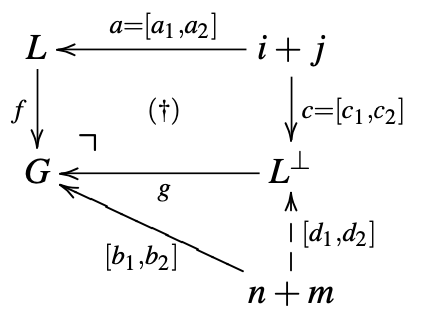
\includegraphics[width=0.3\linewidth]{figures/combinatorial_semantics/boundary_complement.png}
%     \label{fig:boundary_complement}
% \end{figure}

% is called a boundary complement if $[c_1, c_2]$ is mono and there exist $d_1 : n \to L^{\bot}$ and $d_2 : m \to L^{\bot}$ making the above triangle commute and such that
% \[
%     n + j \xrightarrow{[d_1,c_2]} L^{\bot} \xleftarrow{[d_2,c_1]} m + i
% \]
% is a monogamous cospan
% \end{definition}

\subsection{Syntactic rewriting of PROPs}

\Aleksei{Should this be a separate section rather than a subsection?}

\begin{definition}[\cite{Frobenius}]
A rewriting system $\mathcal{R}$ in a PROP $\mathbb{A}$ consists of a set of rewriting rules, i.e. pairs $\langle l , r \rangle$ of morphisms $l , r : i \to j$ in $\mathbb{A}$ with the same arities and co-arities.
Given $a, b : m \to n$ in $\mathbb{A}$, $a$ rewrites into $b$ via $\mathcal{R}$, written $a\Rightarrow_{\mathcal{R}} b$ ,if they are decomposable as in Figure~\ref{fig:prop_rewriting}, for some rule $\langle l,r \rangle \in \mathcal{R}$    
\end{definition}

\begin{figure}[h!]
    
    \[
    \scalebox{0.75}{\tikzfig{combinatorial_semantics/prop_rewriting}}
    \]
    \caption{Rewriting in $\textsf{PROP}(\Sigma)$}
    \label{fig:prop_rewriting}
\end{figure}

\begin{definition}
Given a rewriting system $\mathcal{R}$ for a $\textsf{PROP}(\Sigma)$ we define 
 a rewriting system $\mathcal{R}^{+}$ in a $\textsf{PROP}^{+}(\Sigma)$  as a set of pairs $\langle l , r \rangle$ for each pair $\langle l, r \rangle$ in $\mathcal{R}$.
However, the rewriting happens modulo semilattice enriched laws rather than SMC laws.
We define what $a \Rightarrow_{\mathcal{R}^+} b$ means for some rule $\langle l , r\rangle $ based on the structure of $a$ and $b$.

If they are decomposable as in Figure~\ref{fig:prop_rewriting} then we say that $a$ rewrites to $b$ under rule $\langle l, r \rangle$ in $\mathcal{R}^{+}$.
Another case is when some $a'$ rewrites to some $b'$ under rule $\langle l, r \rangle$ in the sense above ($\Rightarrow_{\mathcal{R}})$)) and then we say that $a$ rewrites to $b$ under the same rule if they are decomposable as in Figure~\ref{fig:enriched_prop_rewriting}.

\begin{figure}

    \[
    \scalebox{0.6}{
    \tikzfig{combinatorial_semantics/prop_plus_rewriting}
    }
    \]
    \caption{Rewriting in $\textsf{PROP}^{+}(\Sigma)$}
    \label{fig:enriched_prop_rewriting}
\end{figure}

\end{definition}



% \update{

% \begin{definition}
%     Functor $\llbracket \cdot \rrbracket : \text{PROP}^{+} \to \catname{MACsp_{D}(EHyp_{\Sigma})}$.

%     We will build this functor inductively. As noted above, $\MdaCospans$ is a full subcategory of $\catname{MACsp_{D}(EHyp_{\Sigma})}$ and the acting of this functor on generators can be found in~\cite{Frobenius}. We need to define what $+$ from $\text{PROP}^{+}$ in $\catname{MACsp_{D}(EHyp_{\Sigma})}$ is. The definition could be found in Figure~\ref{fig:f+g} where well-typed mda-cospans for images of arbitrary morphisms $f, g : m \to n$ are depicted on the left and the image of $f + g$ is depicted on the right. A new edge is introduced which is the immediate predecessor of arbitrary e-hypergraphs $f$ and all edges and nodes of $f$ and $g$ are in conflict. The nodes are added to the interfaces and to the new edge to preserve well-typedness.

% \end{definition}

% }





We will later mimic rewrites in $\textsf{PROP}^{+}(\Sigma)$ at the level of $\WellTypedMdaEcospans$ by utilising a generalisation of double-pushout with interfaces (DPOI) approach defined in~\cite{Frobenius}.
First, we will recall standard double-pushout (DPO) rewriting.

DPO is a technique for formalising rewriting in graph-like categories.
For a given rewrite rule $\langle l, r \rangle$ it corresponds to an intuitive notion of removing an occurrence of $l$ within a graph and then plugging $r$ in there.
More specifically, a DPO rule is a span $L \xleftarrow{} K \xrightarrow{} R$ in some category $\mathcal{C}$ with pushouts, where $L$ stands for the $l$ part of a rewrite rule, $R$ stands for the $r$, and $K$ is the invariant that should be maintained during rewriting.

A typical DPO square looks like this


\[
\begin{tikzcd}
L \arrow[d, "m"'] & K \arrow[d] \arrow[l, "f"'] \arrow[r, "g"] & R \arrow[d]   \\
G^{\urcorner}     & C \arrow[l] \arrow[r]                      & ^{\ulcorner}H
\end{tikzcd}
\]

where the two marked squares are pushouts. Morphisms $K \to C \to G$ are called a \textit{pushout complement} and morphism $m$ is called a \textit{match} and is defined when the corresponding pushout complement exists. When $f,g$ are injective, constructing $C$ can be intuitively understood as finding an occurrence of $L$ in $G$ and removing from this occurrence everything that has no pre-image in $K$ and then inserting in there everything from $R$ that has no pre-image in $K$ (hence the two pushouts: one for deletion and one for insertion). Then we say that $G$ is rewritten into $H$ under a rewrite rule $L \xleftarrow{} K \xrightarrow{} R$. 

However, this notion of DPO does not account for hypergraphs with interfaces, i.e. those from $\MdaCospans$ where $l,r$ from $\langle l, r \rangle$ are cospans. To support this we first assume that we only need to maintain the interfaces of $i \xrightarrow{} L \xleftarrow{} j$ and $i \xrightarrow{} R \xleftarrow{} j$ during rewriting, then we can take $K \cong i + j$, i.e. take $K$ to be the coproduct of $i,j$ (remark 3.14~\cite{Frobenius}). What remains is to account for the interfaces in $G$, $C$, and $H$, which brings us to the following modified DPOI square. $J \cong n + m$ where $n$ and $m$ are the input and output interfaces of $G$, $C$, and $H$ respectively. The only difference from DPO square above is that we now explicitly require that the initial object $G$, intermediate object $C$ and final object $H$ all share the same interfaces.


\[
\begin{tikzcd}
L \arrow[d, "m"'] & K \arrow[d] \arrow[l, "f"'] \arrow[r, "g"] & R \arrow[d]   \\
G^{\urcorner}     & C \arrow[l] \arrow[r]                      & ^{\ulcorner}H \\
                  & J \arrow[lu] \arrow[u] \arrow[ru]          &              
\end{tikzcd}
\]

To mimic rewrites in $\textsf{PROP}(\Sigma)$ we need to put some restrictions on pushout complements as not all of them lead to mda-cospans.

\begin{definition}[Boundary complement for $\catname{MACsp_{D}(Hyp_{\Sigma}))}$]
\label{def:boundary_original}
For monogamous cospans $i \xrightarrow{a_1} L \xleftarrow{a_2} j$ and $n \xrightarrow{b_1} G \xleftarrow{b_2} m$
and mono $f : L \to G$, a pushout complement as depicted below

\begin{figure}[h!]
    \centering
    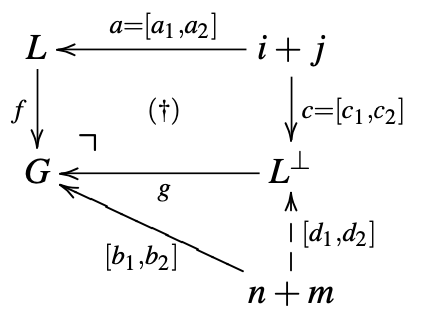
\includegraphics[width=0.3\linewidth]{figures/combinatorial_semantics/boundary_complement.png}
\end{figure}

is called a boundary complement if $[c_1, c_2]$ is mono and there exist $d_1 : n \to L^{\bot}$ and $d_2 : m \to L^{\bot}$ making the above triangle commute and such that
\[
    n + j \xrightarrow{[d_1,c_2]} L^{\bot} \xleftarrow{[d_2,c_1]} m + i
\]
is a monogamous cospan. 
\end{definition}

Intuitively, such a pushout complement requires that inputs get only glued to outputs and vice-verse in the two pushout squares.

\begin{definition}{Convex match}

We call a match $m : L \to G$ convex if it is mono and its image is a convex subgraph of $G$. 
    
\end{definition}

\begin{definition}{Rewriting in $\catname{MACsp_{D}({Hyp_{\Sigma}})}$}

Given $G \xleftarrow{} n+m$ and $H \xleftarrow{} n + m$ in $\catname{Hyp_{\Sigma}}$, $G$ rewrites convexly into $H$ with interface $n + m$ --- notation $(G \xleftarrow{} n + m ) \Rrightarrow_{\mathcal{R}}  (H \xleftarrow{} n + m )$ --- if there exist rule $L \xleftarrow{} i + j \xrightarrow{} R$ in $\mathcal{R}$ and object $C$ and cospan arrows $i+j \xrightarrow{} C \xleftarrow{} n+m$ in $\catname{Hyp_{\Sigma}}$ such that the DPOI diagram above commutes and its marked squares are pushouts and the following conditions hold

\begin{itemize}
    \item $m : L \to G$ is a convex match;
    \item $i + j \to C \to G$ is a boundary complement in the leftmost pushout.
\end{itemize}
    
\end{definition}

\textbf{Update: 4 Oct}

\begin{theorem}[Theorem 35~\cite{Frobenius2}]
\label{theorem:rewriting_no_frob}
    Let $R$ be any rewriting system on $\textsf{PROP}(\Sigma)$. Then,
    \[
    g \Rightarrow_{\mathcal{R}} h \;\text{ iff }\; \llangle ^{\ulcorner}g^{\urcorner} \rrangle \Rrightarrow_{\llangle \mathcal{R} \rrangle} \llangle ^{\ulcorner}h^{\urcorner} \rrangle 
    \]

    where $\llangle \cdot \rrangle : \textsf{PROP}(\Sigma) + Frob \to \catname{Csp_{D}(Hyp_{\Sigma})}$ is an isomorphism of props.
    \update{
        Last time I confused functors $\llangle \cdot \rrangle$ and $\llbracket \cdot \rrbracket$.
        Note that the result above is a weaker version of the same result for rewriting in $\textsf{PROP}(\Sigma) + Frob$.
        $Frob$ is an SMT with the signature $\Sigma_{Frob}$ which constitutes of \textit{only} Frobenius generators and terms are quotiented by both SMC laws and Frobenius equations.
        So, essentially, $Frob = \textsf{PROP}(\Sigma_{Frob}, \mathcal{E}_{Frob})$. 
        \question{Is it true that by quotienting $\textsf{PROP}(\Sigma)$ by SMC laws and quotienting $Frob$ by SMC and Frob laws we automatically quotient $\textsf{PROP}(\Sigma) + Frob$ by SMC and Frob laws?} 
    }
\end{theorem}

\begin{definition}[$\ulcorner \cdot \urcorner$]

    This is a syntactic operation which is defined for terms in $\textsf{PROP}(\Sigma) + Frob$ and is given below
    \[
        \tikzfig{combinatorial_semantics/bending_wires}
    \]
    
\end{definition}

\begin{remark}
    We need the operation above because we defined the rewriting for cospans of hypergraphs only for cospans of the form $0 \to G \xleftarrow{} n + m$ (for $\catname{Csp_{D}(Hyp_{\Sigma})},\; \MdaCospans,\; \MdaEcospans$), but the functors take arbitrary terms (string diagrams) as input.
    This operation turns an arbitrary term into a term with no inputs.
    Now the left-hand and right-hand sides are equivalent in the sense that $f \Rightarrow_{\langle l, r \rangle} g$ if and only if $\ulcorner f \urcorner \Rrightarrow_{\langle \ulcorner l \urcorner, \ulcorner r \urcorner \rangle} 
 \ulcorner g \urcorner$ and the latter string diagram can be interpreted as $0 \xrightarrow{} G \xleftarrow{} n + m$ for which we defined rewriting above.

\end{remark}

\begin{proposition}

    $m \xrightarrow{} \mathcal{G} \xleftarrow{} n$ is mda-cospan in $\MdaCospans$ iff $0 \xrightarrow{} \mathcal{G} \xleftarrow{} n + m$ is an mda-cospan.
\end{proposition}

In particular, the above proposition means that by fullness of $\llbracket \cdot \rrbracket$ there exists a corresponding SMC morphism for some $0 \xrightarrow{} \mathcal{G}\xleftarrow{} n + m$.
Theorem above essentially makes two routes below. In forward direction:

\[
\textsf{PROP}(\Sigma) \xrightarrow{i_1} \textsf{PROP}(\Sigma) + Frob \xrightarrow{\ulcorner \cdot \urcorner} \textsf{PROP}(\Sigma) + Frob \xrightarrow{\llangle \cdot \rrangle} \catname{Csp_{D}(Hyp_{\Sigma})}
\]

The proof of the theorem above in the forward direction then relies on the proof for rewriting in $\textsf{PROP}(\Sigma) + Frob$ and functoriality of $\llangle \cdot \rrangle$ and checking that a match is convex.

In backwards direction

\[
  \catname{Csp_{D}(Hyp_{\Sigma})} \xrightarrow{\llbracket \cdot \rrbracket}^{-1} \textsf{PROP}(\Sigma)  
\]

relies on decomposition of a hypergraph given a convex match and on fullness of 

\[
    \llbracket \cdot \rrbracket : \textsf{PROP}(\Sigma) \to \MdaCospans
\]

\question{What options we have?
\begin{enumerate}
    \item Define $PROP(\Sigma)^{+}$ and $PROP(\Sigma)^{+} + Frob$
    \item Say that $n \xrightarrow{} \mathcal{G} \xleftarrow{} m$ rewrites into $n \xrightarrow{} \mathcal{F} \xleftarrow{} m$ iff $0 \xrightarrow{} \mathcal{G} \xrightarrow{} n + m$ rewrites into $0 \xrightarrow{} \mathcal{F} \xrightarrow{} n + m$.
          This gives the following route
          \[
            \textsf{PROP}(\Sigma)^{+} \xrightarrow{\llbracket \cdot \rrbracket} \MdaEcospans \xrightarrow{\ulcorner \cdot \urcorner} \MdaEcospans
          \]

          and the same in the other direction with flipped arrows.
\end{enumerate}
}
\Aleksei{TODO: discuss this}

If we quotient $\MdaCospans$ by $\llangle \mathcal{R} \rrangle$ by the theorem~\ref{theorem:rewriting_no_frob} and faithfulness and fullness of $\llbracket \cdot \rrbracket$ we get the following result.
$f = g$ in $\textsf{PROP}(\Sigma,\mathcal{E})$ iff $\llangle ^{\ulcorner} f ^{\urcorner} \rrangle = \llangle ^{\ulcorner} f ^{\urcorner} \rrangle$ in $\MdaCospans$.

\question{Do we want the same result for $\textsf{PROP}(\Sigma, \mathcal{E})^{+}$ and $\WellTypedMdaEcospans$?}

\textbf{End of update}

We have a more general notion of interface and hence we need to adjust DPOI rewriting a little bit.
The first issue is that whole interfaces are not preserved during rewriting, consider an example in Figure~\ref{fig:example_rewrite_ecospans} which corresponds to a rewrite rule of $\langle f, f+g \rangle$.

\begin{figure}[t]
    \centering
    \[
    \scalebox{0.6}{\tikzfig{combinatorial_semantics/f_to_f_plus_g_example}}
    \]
    \caption{Example rewrite rule in $\WellTypedMdaEcospans$}
    \label{fig:example_rewrite_ecospans}
\end{figure}

The input interface on the left-hand side of the rule is $\{1, 2\}$, while the input interface on the right-hand side of the rule is $\{1,2,5,6,7,8\}$.
Note that the outermost interfaces are preserved.

Another concern is when we delete the occurrence of the left-hand side of a rewrite rule from an e-hypergraph we also modify this e-hypergraph's interfaces.
Consider a hypothetical DPO square below in Figure~\ref{fig:interface_change_example} where long arrows denote matching between carriers of cospans.

\begin{figure}
    \centering
    \[
    \scalebox{0.5}{\tikzfig{combinatorial_semantics/interfaces_change_example}}\]
    \caption{Hypothetical DPO square for $\catname{MACsp_{D}(EHyp_{\Sigma})}$}
    \label{fig:interface_change_example}
\end{figure}

The first row of the diagram shows the span for a rewrite rule of $\langle f + g, f \rangle$ which is like a projection rule.
Note once again the difference between the interfaces of the left-hand and right-hand sides of the rewrite rule.
The entry in the middle of the span depicts the outermost interfaces which are preserved.
The second row depicts the e-hypergraph to be rewritten on the left and the result of the rewrite on the right.
The result is obtained by first deleting the image of the left-hand side of the rewrite rule from the initial e-hypergraph (depicted in the middle) and then gluing the right-hand side of the rewrite rule into it. 
Note that the interfaces of the initial e-hypergraph and the residual e-hypergraph are different. 
Here, the outermost and the whole interfaces for the eventual e-hypergraph coincide, but if the nested-ness of the initial e-hypergraph was more intense the result could have inner interfaces as well as we would remove the interfaces of the inner edges when deleting the image of the left-hand side part of the rule from the initial e-hypergraph.


\update{$i,j$ are replaced}

To account for such changes in the interfaces we put some additional constraints on DPOI rewriting.
Consider a DPOI diagram with extra constraints below which encodes
 the notion that cospan 
 $n_{ext} \xrightarrow{} g_i \xrightarrow{} G \xleftarrow{} g_o \xleftarrow{} m_{ext}$
 rewrites into a cospan 
 $n_{ext} \xrightarrow{} h_i \xrightarrow{} H \xleftarrow{} h_o \xleftarrow{} m_{ext}$ via a rewrite rule $\langle l, r \rangle$,
 where
 $l := x_{ext} \xrightarrow{} l_i \xrightarrow{} L \xleftarrow{} l_o \xleftarrow{} y_{ext}$
 and
 $r := x_{ext} \xrightarrow{} r_i \xrightarrow{} L \xleftarrow{} r_o \xleftarrow{} y_{ext}$.
 Note there are arrows from $x_{ext} + y_{ext} \to l_i + l_o$ (respectively, $r_i + r_o$) from the corresponding cospans which are not shown in the diagram.
 Similarly for the arrows from $n_{ext} + m_{ext}$.

% \[\begin{tikzcd}
% 	&&&& {i + j} \\
% 	{l_i+l_o} && L &&&& R && {r_i+r_o} \\
% 	\\
% 	{g_i+g_o} && {G^{\urcorner}} && C && {^{\ulcorner}H} && {h_i+h_o} \\
% 	\\
% 	&&&& {n+m}
% 	\arrow[color={rgb,255:red,214;green,92;blue,92}, from=1-5, to=2-3]
% 	\arrow[color={rgb,255:red,214;green,92;blue,92}, from=1-5, to=2-7]
% 	\arrow["m", color={rgb,255:red,214;green,92;blue,92}, from=2-3, to=4-3]
% 	\arrow["{[i_c,j_c]}", color={rgb,255:red,214;green,92;blue,92}, from=1-5, to=4-5]
% 	\arrow[color={rgb,255:red,214;green,92;blue,92}, from=2-7, to=4-7]
% 	\arrow["{[n_c,m_c]}"', color={rgb,255:red,214;green,92;blue,92}, from=6-5, to=4-5]
% 	\arrow[color={rgb,255:red,214;green,92;blue,92}, from=4-5, to=4-7]
% 	\arrow[color={rgb,255:red,214;green,92;blue,92}, from=4-5, to=4-3]
% 	\arrow[color={rgb,255:red,214;green,92;blue,92}, from=6-5, to=4-3]
% 	\arrow[color={rgb,255:red,214;green,92;blue,92}, from=6-5, to=4-7]
% 	\arrow[from=2-1, to=2-3]
% 	\arrow["{[f_i,f_o]}", from=2-1, to=4-1]
% 	\arrow[from=4-1, to=4-3]
% 	\arrow[from=2-9, to=2-7]
% 	\arrow[from=4-9, to=4-7]
% 	\arrow["{[h_i,h_o]}"{description}, from=2-9, to=4-9]
% 	\arrow[from=6-5, to=4-9]
% 	\arrow[from=6-5, to=4-1]
% 	\arrow["{[i_l,j_l]}"{description}, from=1-5, to=2-1]
% 	\arrow["{[i_r,j_r]}"{description}, from=1-5, to=2-9]
% \end{tikzcd}\]


% https://q.uiver.app/#q=WzAsMTEsWzIsMCwiTCJdLFs0LDAsInhfe2V4dH0gKyB5X3tleHR9Il0sWzIsMiwiR157XFx1cmNvcm5lcn0iXSxbNCwyLCJDIl0sWzQsNCwibl97ZXh0fSttX3tleHR9Il0sWzAsMCwibF9pK2xfbyJdLFswLDIsImdfaStnX28iXSxbNiwwLCJSIl0sWzYsMiwiXntcXHVsY29ybmVyfUgiXSxbOCwyLCJoX2kraF9vIl0sWzgsMCwicl9pK3JfbyJdLFsxLDAsIiIsMCx7ImNvbG91ciI6WzAsNjAsNjBdfV0sWzAsMiwibSIsMCx7ImNvbG91ciI6WzAsNjAsNjBdfSxbMCw2MCw2MCwxXV0sWzEsMywiW2lfYyxqX2NdIiwwLHsiY29sb3VyIjpbMCw2MCw2MF19LFswLDYwLDYwLDFdXSxbNCwzLCJbbl9jLG1fY10iLDIseyJjb2xvdXIiOlswLDYwLDYwXX0sWzAsNjAsNjAsMV1dLFszLDIsIiIsMix7ImNvbG91ciI6WzAsNjAsNjBdfV0sWzQsMiwiIiwyLHsiY29sb3VyIjpbMCw2MCw2MF19XSxbNSwwXSxbNiwyXSxbNCw4LCIiLDAseyJjb2xvdXIiOlswLDYwLDYwXX1dLFszLDgsIiIsMCx7ImNvbG91ciI6WzAsNjAsNjBdfV0sWzcsOCwiIiwyLHsiY29sb3VyIjpbMCw2MCw2MF19XSxbMSw3LCIiLDIseyJjb2xvdXIiOlswLDYwLDYwXX1dLFsxMCw3XSxbOSw4XV0=
\[\begin{tikzcd}
	{l_i+l_o} && L && {x_{ext} + y_{ext}} && R && {r_i+r_o} \\
	\\
	{g_i+g_o} && {G^{\urcorner}} && C && {^{\ulcorner}H} && {h_i+h_o} \\
	\\
	&&&& {n_{ext}+m_{ext}}
	\arrow[draw={rgb,255:red,214;green,92;blue,92}, from=1-5, to=1-3]
	\arrow["m", color={rgb,255:red,214;green,92;blue,92}, from=1-3, to=3-3]
	\arrow["{[i_c,j_c]}", color={rgb,255:red,214;green,92;blue,92}, from=1-5, to=3-5]
	\arrow["{[n_c,m_c]}"', color={rgb,255:red,214;green,92;blue,92}, from=5-5, to=3-5]
	\arrow[draw={rgb,255:red,214;green,92;blue,92}, from=3-5, to=3-3]
	\arrow[draw={rgb,255:red,214;green,92;blue,92}, from=5-5, to=3-3]
	\arrow[from=1-1, to=1-3]
	\arrow[from=3-1, to=3-3]
	\arrow[draw={rgb,255:red,214;green,92;blue,92}, from=5-5, to=3-7]
	\arrow[draw={rgb,255:red,214;green,92;blue,92}, from=3-5, to=3-7]
	\arrow[draw={rgb,255:red,214;green,92;blue,92}, from=1-7, to=3-7]
	\arrow[draw={rgb,255:red,214;green,92;blue,92}, from=1-5, to=1-7]
	\arrow[from=1-9, to=1-7]
	\arrow[from=3-9, to=3-7]
\end{tikzcd}\]

The original DPOI square is shown in red.
The extra bits simply account for more complicated interfaces.
For example, the left-hand side $L$ of a rewrite rule
 $\langle L, R \rangle$ which originally was some cospan
 $i \xrightarrow{} L \xleftarrow{} j$ in $\MdaCospans$ 
 now is a cospan
 $x_{ext} \xrightarrow{} l_i \to L \xleftarrow{} l_o \xleftarrow{} y_{ext}$
from $\WellTypedMdaEcospans$ where $l_i, l_o$ are whole input and output interfaces respectively.
The top half of this diagram says that the outermost interfaces
 should coincide for $L$ and $R$.
The bottom half puts the same restrictions on $G$ and $H$. 
% The extra squares on both sides say that there should exist a matching of the interfaces together with a matching of e-hypergraphs. This requirement was implicit in the case of $\catname{MACsp_{D}(Hyp_{\Sigma}}$ because the whole interfaces and the outermost interfaces coincided. Because now the interfaces can change, we need to keep track of which parts of the interfaces are subjected to changes.


We also adjust the definition of a boundary complement a bit.

\begin{definition}[Boundary complement in $\WellTypedMdaEcospans$]
\label{def:boundary_new}

% https://q.uiver.app/#q=WzAsNyxbMiwwLCJMIl0sWzQsMCwieF97ZXh0fSArIHlfe2V4dH0iXSxbMiwyLCJHXntcXHVyY29ybmVyfSJdLFs0LDIsIkMiXSxbNCw0LCJuX3tleHR9K21fe2V4dH0iXSxbMCwwLCJsX2krbF9vIl0sWzAsMiwiZ19pK2dfbyJdLFsxLDAsIiIsMCx7ImNvbG91ciI6WzAsNjAsNjBdfV0sWzAsMiwibSIsMCx7ImNvbG91ciI6WzAsNjAsNjBdfSxbMCw2MCw2MCwxXV0sWzEsMywiW2lfYyxqX2NdIiwwLHsiY29sb3VyIjpbMCw2MCw2MF19LFswLDYwLDYwLDFdXSxbNCwzLCJbbl9jLG1fY10iLDIseyJjb2xvdXIiOlswLDYwLDYwXX0sWzAsNjAsNjAsMV1dLFszLDIsIiIsMix7ImNvbG91ciI6WzAsNjAsNjBdfV0sWzQsMiwiIiwyLHsiY29sb3VyIjpbMCw2MCw2MF19XSxbNSwwXSxbNiwyXV0=
\[\begin{tikzcd}
	{l_i+l_o} && L && {x_{ext} + y_{ext}} \\
	\\
	{g_i+g_o} && {G^{\urcorner}} && C \\
	\\
	&&&& {n_{ext}+m_{ext}}
	\arrow[draw={rgb,255:red,214;green,92;blue,92}, from=1-5, to=1-3]
	\arrow["m", color={rgb,255:red,214;green,92;blue,92}, from=1-3, to=3-3]
	\arrow["{[i_c,j_c]}", color={rgb,255:red,214;green,92;blue,92}, from=1-5, to=3-5]
	\arrow["{[n_c,m_c]}"', color={rgb,255:red,214;green,92;blue,92}, from=5-5, to=3-5]
	\arrow[draw={rgb,255:red,214;green,92;blue,92}, from=3-5, to=3-3]
	\arrow[draw={rgb,255:red,214;green,92;blue,92}, from=5-5, to=3-3]
	\arrow[from=1-1, to=1-3]
	\arrow[from=3-1, to=3-3]
\end{tikzcd}\]

Consider the diagram above where the marked square is a pushout
 and $x_{ext} + y_{ext}$ and $n_{ext} + m_{ext}$ are 
 the \textit{outermost} interfaces for the corresponding 
 cospans.
We say that $x_{ext} + y_{ext} \to C \to G^{\urcorner}$ is 
 a \textit{boundary} complement if $[i_c, i_j]$ is mono 
 and there exist $n_c : n_{ext} \to C$ and $m_c : m_{ext} \to C$ 
 making the above triangle commute and such that
there exists a \textit{not necessarily well-typed} mda-cospan

\[
n_{ext} \xrightarrow{} c_i + y_{ext} \xrightarrow{} C \xleftarrow{} c_o + x_{ext} \xleftarrow{} m_{ext}
\]

where $c_i$ and $c_o$ are computed as
 $c_i = g_i \setminus (l_i \setminus x_{ext})$ and
 $c_o = g_o \setminus (l_o \setminus y_{ext})$.
\end{definition}

% Intuitively, these pushout squares mean that when we delete the occurrence of $L$ from $G$ we also remove the occurrence of $L$'s interface within $G$'s interface preserving the outermost interfaces $i + j$. The highlighted arrows form the pushout square for the original boundary complement.

% We call morphisms $i + j \to C \to G$ a boundary complement if

% \begin{enumerate}
%     \item The square above commutes and $L \xrightarrow{} G \xleftarrow{} C$ is a pushout
%     \item There exists an mda cospan $g_i \setminus (l_i \setminus i) + j \xrightarrow{} C \xleftarrow{} g_o \setminus (l_o \setminus j) + i$. \question{I am unsure about categorical notation for this set difference. Maybe it can be paraphrased in the following way?}
%     \item There exists an mda cospan $c_i + j \xrightarrow{} C \xleftarrow{} c_o + i$ where $c_i$ and $c_o$ are the following pushout complements in the category of discrete hypergraphs:
% \end{enumerate}



% The second point above means that when cutting the mono-occurrence of $L$ out from $G$ we also need to remove the inner interfaces of $L$ from the whole interface of $G$. \question{According to the pushout squares above, $c_i$ is constructed by removing from $g_i$ everything from $l_i$ which does not have a pre-image in $i$, i.e., everything except the outermost interfaces (same holds for $c_o$)}

\begin{remark}
Note that cospan $n_{ext} \xrightarrow{} c_i + y_{ext} \xrightarrow{} C \xleftarrow{} c_o + x_{ext} \xleftarrow{} m_{ext}$ is not well-typed.
The cospan's input interface contains nodes that previously were a part of the output interface.
\end{remark}

First, let's check that this notion generalises the ordinary boundary complement from~\ref{def:boundary_original}.
For this, we assume that child and conflict relations are empty in which case $x_{ext} + y_{ext}$ and $l_i + l_o$ coincide as well as $g_i + g_o$ and $n_{ext} + m_{ext}$.
Hence, $g_i \setminus (l_i \setminus x_{ext}) + y_{ext} = g_i + y_{ext} = n_{ext} + y_{ext}$ and the same for the output interfaces.
Thus we have $n_{ext} + y_{ext} \xrightarrow{} C \xleftarrow{} m_{ext} + x_{ext}$, which corresponds to the definition from~\ref{def:boundary_original}.

% Next, consider an example from figure~\ref{fig:dpoir}. The outermost interfaces of $L$ coincide with the whole interfaces, i.e. $l_i + l_o = i + j$. However, $n + m = \{0'', 1''\}$ and $g_i + g_o = \{0'',0,2,1,3,1''\}$. According to the definition of a boundary complement the following mda cospan should exist: $g_i \setminus (l_i \setminus i) + j = \{0'', 0, 2\} \setminus \varnothing \cup \{1\} = \{0'',0,2,1\} \xrightarrow{} C \xleftarrow{} \{0,1,3,1''\} = \text{same procedure for output interfaces}$.

% \question{We need to show that this boundary complement is unique and that after performing a pushout on the right the result is also an mda hypergraph}

% We can now present a complete DPOI square

% \[
% \begin{tikzcd}
%                    &                    & i+j \arrow[ld] \arrow[lld] \arrow[ddd, "f"] \arrow[rrd] \arrow[rd] &                    &              &  &                       &               &                       &               \\
% L \arrow[dd, "m"'] & l_i+l_o \arrow[l]  &                                                                    & r_i+r_j \arrow[r]  & R \arrow[dd] &  & i \arrow[r] \arrow[d] & r_i \arrow[d] & j \arrow[d] \arrow[r] & r_o \arrow[d] \\
%                    &                    &                                                                    &                    &              &  & c_i \arrow[r]         & h_i           & c_o \arrow[r]         & h_o           \\
% G                  &                    & C \arrow[ll] \arrow[rr]                                            &                    & H            &  &                       &               &                       &               \\
%                    & g_i+g_o \arrow[lu] & n+m \arrow[u] \arrow[l] \arrow[llu] \arrow[r] \arrow[rru]          & h_i+h_o \arrow[ru] &              &  &                       &               &                       &              
% \end{tikzcd}
% \]



% \begin{remark}
%     Note that in all pushout squares for the interfaces all the morphisms are monos. \question{Does it follow from anything above? Because the corresponding triangles commute?}
% \end{remark}



\begin{proposition}
    The boundary complement in~\ref{def:boundary_new} when exists is unique
    \begin{proof}
        \update{TODO}
    \end{proof}
\end{proposition}


\question{
\begin{definition}[Convex down-closed conflict reflecting match] 
    We call $m : L \to G$ in $\catname{EHyp_{\Sigma}}$ a convex down-closed conflict reflecting match if
    
    \begin{enumerate}
        \item $m$ is monomorphism
        \item $m(L)$ is a convex down-closed subgraph of $G$
        \item if $m(x_1) \# m(x_2)$ then $x_1 \# x_2$
    \end{enumerate}
\end{definition}
}


\begin{definition}[Rewriting in $\WellTypedMdaEcospans$]
    Given $G \xleftarrow{} g_i + g_o \xleftarrow{} n_{ext} + m_{ext}$ 
    and $H \xleftarrow{} h_i + h_o \xleftarrow{} n_{ext} + m_{ext}$ in $\WellTypedMdaEcospans$ with the outermost interfaces $n_{ext} + m_{ext}$, $G$ rewrites convexly into $H$ with the outermost interface $n_{ext} + m_{ext}$ --- notation $( G \xleftarrow{} n_{ext} + m_{ext} ) \Rrightarrow_{\mathcal{R}} (E \xleftarrow{} n_{ext} + m_{ext} )$ --- if there exists a rule $l_i + l_o \xrightarrow{} L \xleftarrow{} x_{ext} + y_{ext} \xrightarrow{} R \xleftarrow{} r_i + r_o$ with the outermost interfaces $x_{ext} + y_{ext}$ in $\mathcal{R}$ and object $C$ and cospan arrows $x_{ext} + y_{ext} \xrightarrow{} C \xleftarrow{} n_{ext} + m_{ext}$ in $\Ecospans$ such that the diagram below commutes and its marked squares are pushouts

% https://q.uiver.app/#q=WzAsMTEsWzIsMCwiTCJdLFs0LDAsInhfe2V4dH0gKyB5X3tleHR9Il0sWzIsMiwiR157XFx1cmNvcm5lcn0iXSxbNCwyLCJDIl0sWzQsNCwibl97ZXh0fSttX3tleHR9Il0sWzAsMCwibF9pK2xfbyJdLFswLDIsImdfaStnX28iXSxbNiwwLCJSIl0sWzYsMiwiXntcXHVsY29ybmVyfUgiXSxbOCwyLCJoX2kraF9vIl0sWzgsMCwicl9pK3JfbyJdLFsxLDAsIiIsMCx7ImNvbG91ciI6WzAsNjAsNjBdfV0sWzAsMiwibSIsMCx7ImNvbG91ciI6WzAsNjAsNjBdfSxbMCw2MCw2MCwxXV0sWzEsMywiW2lfYyxqX2NdIiwwLHsiY29sb3VyIjpbMCw2MCw2MF19LFswLDYwLDYwLDFdXSxbNCwzLCJbbl9jLG1fY10iLDIseyJjb2xvdXIiOlswLDYwLDYwXX0sWzAsNjAsNjAsMV1dLFszLDIsIiIsMix7ImNvbG91ciI6WzAsNjAsNjBdfV0sWzQsMiwiIiwyLHsiY29sb3VyIjpbMCw2MCw2MF19XSxbNSwwXSxbNiwyXSxbNCw4LCIiLDAseyJjb2xvdXIiOlswLDYwLDYwXX1dLFszLDgsIiIsMCx7ImNvbG91ciI6WzAsNjAsNjBdfV0sWzcsOCwiIiwyLHsiY29sb3VyIjpbMCw2MCw2MF19XSxbMSw3LCIiLDIseyJjb2xvdXIiOlswLDYwLDYwXX1dLFsxMCw3XSxbOSw4XV0=
\[\begin{tikzcd}
	{l_i+l_o} && L && {x_{ext} + y_{ext}} && R && {r_i+r_o} \\
	\\
	{g_i+g_o} && {G^{\urcorner}} && C && {^{\ulcorner}H} && {h_i+h_o} \\
	\\
	&&&& {n_{ext}+m_{ext}}
	\arrow[draw={rgb,255:red,214;green,92;blue,92}, from=1-5, to=1-3]
	\arrow["m", color={rgb,255:red,214;green,92;blue,92}, from=1-3, to=3-3]
	\arrow["{[i_c,j_c]}", color={rgb,255:red,214;green,92;blue,92}, from=1-5, to=3-5]
	\arrow["{[n_c,m_c]}"', color={rgb,255:red,214;green,92;blue,92}, from=5-5, to=3-5]
	\arrow[draw={rgb,255:red,214;green,92;blue,92}, from=3-5, to=3-3]
	\arrow[draw={rgb,255:red,214;green,92;blue,92}, from=5-5, to=3-3]
	\arrow[from=1-1, to=1-3]
	\arrow[from=3-1, to=3-3]
	\arrow[draw={rgb,255:red,214;green,92;blue,92}, from=5-5, to=3-7]
	\arrow[draw={rgb,255:red,214;green,92;blue,92}, from=3-5, to=3-7]
	\arrow[draw={rgb,255:red,214;green,92;blue,92}, from=1-7, to=3-7]
	\arrow[draw={rgb,255:red,214;green,92;blue,92}, from=1-5, to=1-7]
	\arrow[from=1-9, to=1-7]
	\arrow[from=3-9, to=3-7]
\end{tikzcd}\]
    and the following conditions hold

    \begin{enumerate}
        \item $m : L \to G$ is a convex down-closed conflict reflecting match;
        \item $x_{ext} + y_{ext} \to C \to G$ is a boundary complement in the leftmost pushout.
    \end{enumerate}
\end{definition}


\Aleksei{Do we need to introduce substitution? This is needed if our rewrite rules are going to have variables as labels.}


The whole interfaces of the resulting e-hypergraph $H$ from the cospan
 $n_{ext} \xrightarrow{} h_i \xrightarrow{} H \xleftarrow{} h_o \xleftarrow{} m_{ext}$
 are constructed as $h_i = (r_i \setminus x_{ext}) + c_i$ 
 and
 $h_o = (r_o \setminus y_{ext}) + c_o$.
 $h_i \to H$ is defined as a copairing of 
 $f_1 : r_i \setminus x_{ext} \to R \to H$ 
 and 
 $f_2 : c_i \to C \to H$. 
Since both $f_1$ and $f_2$ are mono, their copairing is also a mono. 
Similarly for $h_o$.

% using the two pushout squares below.
% Intuitively, these squares combine the interfaces of $R$ and $C$ and identify those bits that share the same pre-image in the outermost interface $i + j$.

% \[\begin{tikzcd}
% i \arrow[r] \arrow[d] & r_i \arrow[d] & j \arrow[r] \arrow[d] & r_o \arrow[d] \\
% c_i \arrow[r]         & h_i           & c_o \arrow[r]         & h_o          
% \end{tikzcd}\]

% Going back to the example from the figure~\ref{fig:dpoir}, $h_i = \{0'',0,0',2',2\}$, $r_i = \{0,0',2'\}$, $r_o = \{1',3',1\}$, $h_o = \{1',3',3,1,1''\}$, $c_i = \{0'',2,0\}$, $c_o = \{1'',1,3\}$, $i = \{0\}$, $j = \{1\}$, where $h_i$ is exactly $c_i \coprod_{\equiv_{i}} r_i = \{0'',2,0\} \coprod_{\equiv_{i}} \{0,0',2'\} = \{0'',0,0',2',2\}$ and the same for $h_o$. 

\begin{proposition}

$n_{ext} \xrightarrow{n_h} h_i \xrightarrow{f} H \xleftarrow{g} h_o \xleftarrow{m_h} m_{ext}$ is a well-typed mda-cospan.

\begin{proof}
$f$ and $g$ are monos by construction.
$n_{ext} + m_{ext} \to h_i + h_o$ is a mono by commutativity because $n_{ext} + m_{ext} \to H$ is a mono (also by commutativity). 
The only in-degree 0 nodes have a pre-image in $c_i$ and $r_i \setminus x_{ext}$  and end up being in the image of $h_i$ (the nodes with the pre-image in $y_{ext}$ get glued together).
Well-typedness is restored once the right-hand side of the rewrite rule is glued into $C$.
\question{Uniqueness of this pushout complement? Is it a presheaf? As a presheaf category is adhesive, $\catname{Csp_{D}(EHyp)}$ can not be a presheaf as it is not adhesive.}
\end{proof}
\end{proposition}

\Aleksei{Check the proof}

\begin{lemma}(Decomposition). Let $m \xrightarrow{} G \xleftarrow{} n$ be a monogamous acyclic cospan and $L$ a convex and down-closed sub-hypergraph of $G$. Then there exists $k \in \mathcal{N}$ and a unique cospan $i \xrightarrow{} L \xleftarrow{} j$ such that G factors as $\ldots$

\update{TODO: this lemma is needed to prove soundness of rewriting}
\end{lemma}

\Aleksei{Can we reuse anything from~\cite{Frobenius}?}


Consider an example below that illustrates the introduced constraints.

\update{I've switched to $[ \cdot ]$ for our functor to be able to differenciate between $\llbracket \cdot \rrbracket$, $\llangle \cdot \rrangle$}
\begin{remark}
    For now, we will informally denote a combinatorial interpretation of a morphism $f$ in $\textsf{PROP}^{+}(\Sigma)$ as $[ f ]$.
\end{remark}

\begin{example}

A DPOI square for rewriting in $\WellTypedMdaEcospans$ is depicted in Figure~\ref{fig:refined_dpoi}.
A projection rule of $\llbracket f + g \rrbracket \to \llbracket f \rrbracket$ is shown in the top half of the diagram.
The image of the matching $m$ is shown in red and its image is a convex down-closed e-hypergraph.
Pushout complement is then computed by removing the image of $m$ from the target e-hypergraph by keeping intact the nodes that have a pre-image in the carrier of the rewriting span. The corresponding mda-cospan is depicted at the bottom: $c_i = g_i \setminus (l_i \setminus i) = \{18, 19, 1, 2, 13, 14, 5, 6, 7, 8\} \setminus (\{1,2,5,6,7,8\} \setminus \{1,2\}) = \{18, 19, 1, 2, 13, 14, 5, 6, 7, 8\} \setminus \{5,6,7,8\} = \{18,19,1,2,13,14\}$ and $c_i + j = \{18,19, 1, 2, 13, 14, 3, 4\}$ which is the input interface for $C$. Similar computations are performed for $c_o$. Then pushout glues $R$ and $C$ together along $i + j$ and the resulting interface $h_i = c_i + (r_i \setminus i) = \{18,19, 1, 2, 13, 14\} + \varnothing = \{18,19, 1, 2, 13, 14\}$ and likewise for $h_o$.

%     \begin{figure}
%         \centering
% \[
%   \scalebox{0.3}{      \tikzfig{combinatorial_semantics/refined_dpoi_example}
% }
%         \]
%     \caption{Refined DPOI rewriting}
%     \label{fig:refined_dpoi}
%     \end{figure}
    
\end{example}

\Aleksei{This figure yeilds "Dimension too large". Need to fix it.}

Unlike SMC equations the equations for semilattice enriched categories are not absorbed by e-hypergraph representation and hence to further build a correspondence between $\textsf{PROP}^{+}(\Sigma)$ and $\WellTypedMdaEcospans$ we add them as structural rewrite rules.
Recall that the category $\catname{EHyp_{\Sigma}}$ does not have all pushouts and hence we need to explicitly show that the pushouts that we need exist.


\begin{proposition}
Pushouts for all semilattice enrichment equations exist.

\begin{proof}
    Let us give a combinatorial interpretation for an instance of the first equation (distributivity) in~\ref{fig:string-equations}.
    It can be found in Figure~\ref{fig:distributivity_interpretation}.
    After we identify a convex down-closed image of the left-hand side of this rule within a graph $G$ we remove the image by keeping only the outermost nodes.
    Then we simply glue the right-hand side of the rule into the hole.
    Since we glue along the outermost nodes this does not introduce any conflict with regard to child relation.
    Such equations are not absorbed by e-hypergraph representation unlike SMC equations because the right-hand side contains more edges, i.e. graphs $G$ and $H$ are not isomorphic.
    Similar argument applies to other rules as well.

\end{proof}
\end{proposition}

\update{I think I haven't paid any attention to this fact previously, but it seems that in~\cite{Frobenius} the functor $\llbracket - \rrbracket$ is between $PROP_{\Sigma_{Frob}}$ and $Csp_{D}(Hyp_{\Sigma})$, i.e. PROP is quotiented by Frobenius equations, but they are absorbed in hypergraphs domain. We will have a similar thing: $\llbracket - \rrbracket: PROP^{+}_{\Sigma^{+}} \to \WellTypedMdaEcospans_{R^+}$, i.e. we will quotient PROP$^{+}$ by semilattice equations and quotient e-hypergraphs by the interpretation of these equations as they are not absorbed. The quotienting on the left is always implicit?}

\begin{figure}
    \centering
    \[
    \scalebox{0.45}{
    \tikzfig{combinatorial_semantics/structural_rule_pushout}}\]  
    \caption{Distributivity rewrite rule interpretation}
    \label{fig:distributivity_interpretation}
\end{figure}

\begin{definition}
    We will denote with $\mathcal{S}$ the interpretation of the equations in~\ref{fig:string-equations} as rewrite rules in $\WellTypedMdaEcospans$.
    In particular, for all $l = r$ in~\ref{fig:string-equations}, $\mathcal{S}$ will contain $\langle [l], [r]\rangle$ and $\langle [r], [l] \rangle$.
    \update{Technically we add those for all possible instances of $l$ and $r$ in~\ref{fig:string-equations}.}
\end{definition}


\begin{remark}
    There is a minor limitation for DPOI rewriting above. It is unable to express rewriting for rules that contain an edge with no inputs and outputs on their right-hand side. This is because there is no way to impose both conflict and child relation of such an edge as it has no incident nodes in its context. An example of this could be seen in Figure~\ref{fig:non_expressible}. After an image of a match is removed there is no way of plugging $k$ into the hierarchical edge as it has no connection with this edge via the shared interface. However, we think that this is only a minor limitation because in practice such edges with no incident nodes correspond to `scalars' if we consider for example a category of vector spaces where a rewrite rule with a scalar could be

\begin{alignat*}{3}
\begin{pmatrix}
 1 &  2 \\
-1 &  1 \\
\end{pmatrix}
&\!\begin{aligned}
\hspace{1em} & \otimes &
\end{aligned}
&\!\begin{aligned}
2 &
\end{aligned}
&\!\begin{aligned}
 & \xrightarrow{} & 
\end{aligned}
&\!\begin{aligned}
\begin{pmatrix}
 2 &  4 \\
-2 &  2 \\
\end{pmatrix}    
\end{aligned}
\end{alignat*}
\end{remark}

That is, typically such scalars are absorbed and not present on the right-hand side of a rewrite rule.

\begin{figure}
    \centering
\[
\scalebox{0.5}{
\tikzfig{combinatorial_semantics/non_expressible_rewrite}
}
\]
    \caption{Non expressible rewrite}
    \label{fig:non_expressible}
\end{figure}

\newpage



\bibliographystyle{acm}
\bibliography{../../bibliography}

\appendix

\ifdefined\ONECOLUMN
% \section{}
\section{$\catname{SLat}$}
\else
\subsection{$\catname{SLat}$}
\fi
\label{sec:appendix:slat}

In this section we define the category of semilattices that we use as a base for enrichment throughout the paper.

\begin{definition}[Semilattice]
    A \textit{semilattice} is a set equipped with an operation that we denote as $+$ which is associative, commutative and idempotent.
  \end{definition}
  
  Note that we do not require the existence of a unit for $+$. 
  Semilattices that satisfy this extra requirement are sometimes called \textit{bounded}, i.e., they are idempotent commutative monoids.
  
  \begin{definition}[Semilattice homomorphism]
  
  A homomorphism between two semilattices $S_{1}$ and $S_{2}$ is a map $h$ that respects $+$.
  That is, for all $s,s' \in S_{1}$, $h(s +_{S_{1}} s') = h(s) +_{S_{2}} h(s')$.
  \end{definition}
  
  \begin{definition}[Category of semilattices]
    
  Semilattices with their respective homomorphisms form a category that we denote $\catname{SLat}$.
  \end{definition}
  
  \begin{proposition}
    $\catname{SLat}$ is a closed symmetric monoidal category.
  \end{proposition}
  \begin{proof}
    The tensor product of two semilattices $S_{1}$ and $S_{2}$ is defined as follows.
    $S_{1} \otimes S_{2}$ consists of pairs $(s_1,s_2)$ $s_{1} \in S_{1}$, $s_{2} \in S_{2}$ quotiented by commutativity, idempotence and associativity and additionally by the following relations
    \begin{itemize}
      \item $(s_{1} +_{S_{1}} s_{1}',s_{2}) \equiv (s_{1},s_{2}) +_{S_{1} \otimes S_{2}} (s_{1}',s_{2})$
      \item $(s_{1}, s_{2} +_{S_{2}} s_{2}') \equiv (s_{1},s_{2}) +_{S_{1} \otimes S_{2}} (s_{1}',s_{2})$
    \end{itemize}
  
    Note that this construction does not identify $(s_1,s_2) +_{S_1 \otimes S_2} (s_1',s_2')$ and $(s_1 +_{S_1} s_1', s_2 +_{S_2} s_2')$.
    The unit for this tensor product is $I = \{*\}$ --- a one-element semilattice.
    Clearly $S \otimes I \cong S$ by mapping $(s,*) \mapsto s$ for all $s \in S$ and vice versa.
    The symmetry, associators and unitors are then obvious morphisms.
    Finally, the category is closed since the set of homomorpisms between two semilattices is a semilattice by defining $(f + g)(x)$ as $f(x) + g(x)$.
    $f + g$ is a homomorphism since $(f + g)(x+y) = f(x+y) + g(x+y) = f(x) + f(y) + g(x) + g(y) = f(x) + g(x) + f(y) + g(y) = f(x+y) + g(x+y)$.
  \end{proof}
  
  This makes $\catname{SLat}$ a suitable base for enrichment.
%    and allows us to take $\mathcal{V} = \catname{SLat}$.

  \begin{definition}
    Forgetful functor $U : \catname{SLat} \to \catname{Set}$ is given by $\catname{SLat}(I_{\catname{SLat}, -}) : \catname{SLat} \to \catname{Set}$.
    \end{definition}
    
    Intuitively, the above functor returns the underlying set of a given semilattice $S$ as each morphism from $\{*\} \to S$ picks out an element of $S$.
    
    \begin{proposition}[Special case of Proposition 6.4.6~\cite{Borceux_1994}]
      The forgetful functor $U : \catname{SLat} \to \catname{Set}$ has a left adjoint free functor $F : \catname{Set} \to \catname{SLat}$.
    \end{proposition}
    \begin{proof}
      The functor $F$ is defined by letting $F(A) = \coprod_{A} I_{\catname{SLat}}$ where the latter is a coproduct which is a `free' product of semilattices defined as follows.
      The elements of $S_{1} \coprod S_{2}$ are sequences $s_{1} + s_{2} + \ldots + s_{n}$ where each $s_{i}$ is either from $S_{1}$ or $S_{2}$ quotiented by all relations in $S_{1}$ and $S_{2}$ and by the necessary equations to turn it into a semilattice.
      The adjunction is then given by the following natural isomorphisms
      \begin{align*}
      \catname{SLat}(\coprod_{A}(I_{\catname{SLat}}), B) &\cong \prod_{A}(\catname{SLat}(I_{\catname{SLat}}, B))\\
                                                         &\cong \catname{Set}(A,\catname{SLat}(I_{\catname{SLat}}, B))\\
                                                         &\cong \catname{Set}(A, U(B))
      \end{align*}
      The first isomorphism is given by the fact that hom-functor makes limits into colimits in its first argument, the second being given by the property that $|\catname{Set}(A,B)| = |B|^{|A|} = |\underbrace{B \times \ldots \times B}_{|A|}|$, and the last isomorphism is given by the definition of $U$.
      Furthermore, we have, 
      \[
      F(I) \cong I_{\catname{SLat}}
      \]
      and 
      \begin{align*}
      F(A) \otimes F(B) &\cong (\coprod_{A} I_{\catname{SLat}}) \otimes (\coprod_{B} I_{\catname{SLat}})\\
            &\cong \coprod_{A} (I_{\catname{SLat}} \otimes \coprod_{B} I_{\catname{SLat}})\\
            &\cong \coprod_{A} (\coprod_{B} (I_{\catname{SLat}} \otimes I_{\catname{SLat}}))\\
            &\cong \coprod_{A} (\coprod_{B} I_{\catname{SLat}})\\
            &\cong \coprod_{A \times B} I_{\catname{SLat}}\\
            &\cong F(A \times B)
      \end{align*}
    In the above we used the fact that functors $- \otimes X$ and $X \otimes -$ preserve colimits as they are both left-adjoint by symmetry and monoidal closedness of $\catname{SLat}$.
    \end{proof}

    \begin{definition}
        Given two $\catname{SLat}$-functors $F,G : \mathbb{C} \to \mathbb{D}$ a $\catname{SLat}$-natural transformation is family of morphisms indexed by objects in $\mathbb{C}$, $\alpha_{A} : I_{\catname{SLat}} \to \mathbb{D}(FA,GA)$ in $\catname{SLat}$ such that the following diagram commutes
        \[
        \adjustbox{width=\linewidth}{
        \begin{tikzcd}
          & {\mathbb{C}(A,A')\otimes I_{\mathcal{V}}} && {\mathbb{D}(FA,FA') \otimes \mathbb{D}(FA',GA')} \\
          {\mathbb{C}(A,A')} &&&& {\mathbb{D}(FA,GA')} \\
          & {I_{\mathcal{V}} \otimes \mathbb{C}(A,A')} && {\mathbb{D}(FA,GA) \otimes \mathbb{D}(GA,GA')}
          \arrow["{G_{A,A'}\otimes \alpha_{A'}}"', from=1-2, to=1-4]
          \arrow["{c_{FA,FA',GA'}}"', from=1-4, to=2-5]
          \arrow["{r^{-1}}", from=2-1, to=1-2]
          \arrow["{l^{-1}}", from=2-1, to=3-2]
          \arrow["{\alpha_{A} \otimes F_{A,A'}}", from=3-2, to=3-4]
          \arrow["{c_{FA,GA,GA'}}", from=3-4, to=2-5]
      \end{tikzcd}}
      \]
      \end{definition}

      Intuitively, in the case of free enrichment $\alpha_{A}$ picks a usual natural transformation from $\mathbb{D}(FA,GA)$.
      
      \begin{example}
        Consider a copy natural transformation $\triangle_{A} : A \to A \times A$ of $\catname{S}(\Sigma_{C},\mathcal{E}_{C})$.
        The later Cartesian PROP is lifted to a Cartesian $\catname{SLat}$-PROP where the naturality condition can be traced component-wise where ${*}$ is a one element semilattice:
      
      \[\adjustbox{width=\linewidth}{
      \begin{tikzcd}  
          & {f + g \otimes *} && {\triangle_{A} \otimes ((f+g) \times (f+g))}\\
          f + g &&&& {\triangle_{A'};((f + g) \times (f+g)) = (f + g);\triangle_{A'}}\\
          & {* \otimes f + g} && {f + g \otimes \triangle_{A'}}
          \arrow[from=1-2, to=1-4]
          \arrow[from=1-4, to=2-5]
          \arrow[from=2-1, to=1-2]
          \arrow[from=2-1, to=3-2]
          \arrow[from=3-2, to=3-4]
          \arrow[from=3-4, to=2-5]
      \end{tikzcd}}
      \]
      
      which is the usual naturality condition.
      
      \end{example}
      
\ifdefined\ONECOLUMN
\section{Proofs for Section \ref{sec:e-hypergraphs}: E-hypergraphs}
\else
\subsection{Proofs for Section \ref{sec:e-hypergraphs}: E-hypergraphs}
\fi
\label{sec:appendix:pushout}

In this section we define the conditions under which the pushout in $\catname{EHyp}(\Sigma)$ exists, and we explicitly construct such a pushout.
We also show the uniqueness of a boundary pushout complement.
These condition will play a crucial role in showing that for each enrichment equation in $\textbf{PROP}^{+}(\Sigma)$ there is a sequence of rewrites in $\WellTypedMdaEcospans$.

\begin{proposition}
    Two cospans in $\catname{Hyp}(\Sigma)$ (\textit{i.e.}, morphisms in $\HypI{\Sigma}$) $n \xrightarrow{f} \mathcal{G} \xleftarrow{g} m$ and $n \xrightarrow{f'} \mathcal{G}' \xleftarrow{g'} m$ are equal if and only if
    the following two cospans  $\catname{EHyp}(\Sigma)$ (\textit{i.e.} morphisms in $\Ecospans$)
    \[
    n \xrightarrow{f_{ext}} n \xrightarrow{f_{int}} \mathcal{G} \xleftarrow{g_{int}} m \xleftarrow{g_{ext}} m
    \]
    \[
        n \xrightarrow{f_{ext}'} n \xrightarrow{f_{int}'} \mathcal{G} \xleftarrow{g_{int}'} m \xleftarrow{g_{ext}'} m    
    \]
    such that $f = f_{ext};f_{int}, f'=f_{ext}';f_{int}'$ (respectively, $g = g_{ext};g_{int}, g' = g_{ext}';g_{int}'$) are equal.
\end{proposition}
This essentially means that $\catname{\HypI{\Sigma}}$ faithfully embeds into $\Ecospans$. 
\begin{proof}
    Recall that cospans are equal when they are isomorphic.
    The proposition means that the following cospans are isomorphic (where $\alpha$ is an isomorphism)
    \[\begin{tikzcd}
            & \mathcal{G} \arrow[dd, "\alpha"] &                                                            \\
    n \arrow[ru, "f", bend left] \arrow[rd, "f'"', bend right] &                                  & m \arrow[lu, "g"', bend right] \arrow[ld, "g'", bend left] \\
            & \mathcal{G}'                     &                                                           
    \end{tikzcd}
    \]
    if and only if the following cospans are isomorphic
    \[
        \begin{tikzcd}
            & n \arrow[r, "f_{int}"] \arrow[dd, "\beta"] & \mathcal{G} \arrow[dd, "\alpha"] & m \arrow[l, "g_{int}"'] \arrow[dd, "\gamma"] &                                                                        \\
n \arrow[ru, "f_{ext}", bend left] \arrow[rd, "f_{ext}'"', bend right] &                                            &                                  &                                              & m \arrow[lu, "g_{ext}"', bend right] \arrow[ld, "g_{ext}'", bend left] \\
            & n \arrow[r, "f_{int}'"']                    & \mathcal{G}'                     & m \arrow[l, "g_{int}'"]                      &                                                                       
\end{tikzcd}    
    \]
    such that $f = f_{ext};f_{int}, f'=f_{ext}';f_{int}'$ (respectively, $g = g_{ext};g_{int}, g' = g_{ext}';g_{int}'$).
    The direction from right to left is straightforward: since the bottom diagram commutes $f;\alpha = f_{int};f_{ext};\alpha = f_{int}';f_{ext}' = f'$ and similarly for $g$.
    
    Let's show the direction from left to right.
    Note that $f_{ext}$ and $f_{ext}'$ have inverses since they are injective and surjective (the injection is per the definition and surjection is because domain and codomain are equal).
    Then we need $f_{ext};\beta = f_{ext}'$ and we define $\beta = f_{ext}^{-1};f_{ext}'$.
    Similarly, $\beta^{-1} = f_{ext}'^{-1};f_{ext}$. 
    We can check that $\beta^{-1};\beta = f_{ext}'^{-1};f_{ext};f_{ext}^{-1};f_{ext}' = f_{ext}'^{-1};id;f_{ext}' = f_{ext}'^{-1};f_{ext}' = id$.
    Then we have that $f_{ext};\beta;f_{int}' = f_{ext};f_{ext}^{-1};f_{ext}';f_{int}' = f_{ext}';f_{int}' = f' = f;\alpha = f_{ext};f_{int};\alpha$.
    Since $f_{ext}$ is surjective, we have $\beta;f_{int}' = f_{int};\alpha$.
    Analogously for $\beta^{-1}$ and the right-hand sides of the diagrams.
\end{proof}

\ifdefined\ONECOLUMN
\section{Existence of pushout}
\else
\subsection{Existence of pushout}
\fi

In constructing the pushout the functional versions of e-hypergraph relations will be useful.
\begin{remark}
    Both $<$ and $\consistency$ can be considered as (partial) functions defined on $V_{\mathcal{F}} + E_{\mathcal{F}}$, \textit{i.e.}, on the coproduct of vertices and edges.
    To make things well-typed, we will use corresponding coproduct injections $\iota_{V} : {V_{\mathcal{F}}} \to V_{\mathcal{F}} + E_{\mathcal{F}}$ and $\iota_{E} : {E_{\mathcal{F}}} \to V_{\mathcal{F}} + E_{\mathcal{F}}$ when passing either a vertex or an edge into these functions.
    For example, an immediate successor of a vertex $x$ can be written functionally as $<_{\mathcal{F}}^{\mu}(\iota_{V_{\mathcal{F}}}(x))$.
\end{remark}

\begin{remark}
    Using functional notation we can reformulate the notion of a homomorphism between two e-hypergraphs in the following way.
\end{remark}
\begin{definition}
        \label{def:e-homo-2}    
        A \emph{homomorphism} $\phi: \mathcal{F} \to \mathcal{G}$ of e-hypergraphs $\mathcal{F},\mathcal{G}$ is a pair of functions $\phi_V : V_{\mathcal{F}} \to V_{\mathcal{G}}, \phi_E : E_{\mathcal{F}} \to E_{\mathcal{G}}$ such that
        
        \begin{enumerate}
            \item $\phi$ is hypergraph homomorphism.
            
            \item When $x$ is not a top-level vertex, 
                \[
                \phi_{E}(<_{\mathcal{F}}^{\mu}(\iota_{V_{\mathcal{F}}}(x))) = <_{\mathcal{G}}^{\mu}(\phi_{V};\iota_{V_{\mathcal{G}}}(x))
                \]
                and
                \[
                \phi_{E}(<_{\mathcal{F}}^{\mu}(\iota_{E_{\mathcal{F}}}(x))) = <_{\mathcal{G}}^{\mu}(\phi_{E};\iota_{E_{\mathcal{G}}}(x))  
                \] when $x$ is a not top-level edge.
                \item
            When $x \in E_{\mathcal{F}}$
            \[
                [\phi_{V};\iota_{V_{\mathcal{G}}}, \phi_{E};\iota_{E_{\mathcal{G}}} ]^{*}(\consistency_{\mathcal{F}}(\iota_{E_{\mathcal{F}}}(x)))
                \subseteq
                \consistency_{\mathcal{G}}(\phi_{E};\iota_{E_{\mathcal{G}}}(x))
            \]
            where $\phi_{V};\iota_{V_{\mathcal{G}}} : V_{\mathcal{F}} \to V_{\mathcal{G}} + E_{\mathcal{G}}$, and similarly for $\phi_{E};\iota_{E_\mathcal{G}}$ so that $[\phi_{V};\iota_{V_{\mathcal{G}}}, \phi_{E};\iota_{E_{\mathcal{G}}}] : V_{\mathcal{F}} + E_{\mathcal{F}} \to  V_{\mathcal{G}} + E_{\mathcal{G}}$.
            \item When $x \in V_{\mathcal{F}}$
            \[
                [\phi_{V};\iota_{V_{\mathcal{G}}}, \phi_{E};\iota_{E_{\mathcal{G}}}]^{*}(\consistency_{\mathcal{F}}(\iota_{V_{\mathcal{F}}}(x)))
                \subseteq
                \consistency_{\mathcal{G}}(\phi_{V};\iota_{V_{\mathcal{G}}}(x)).
            \]
            \end{enumerate}
\end{definition}

\begin{theorem}[Existence of pushouts in $\catname{EHyp}(\Sigma)$]
\label{th:existence_of_pushouts}
Consider the following span in $\catname{EHyp}(\Sigma)$
% https://q.uiver.app/#q=WzAsMyxbMCwwLCJaIl0sWzIsMCwiWCJdLFswLDIsIlkiXSxbMCwxLCJmIl0sWzAsMiwiZyIsMl1d
\[\begin{tikzcd}
	Z && X \\
	\\
	Y
	\arrow["f", from=1-1, to=1-3]
	\arrow["g"', from=1-1, to=3-1]
\end{tikzcd}\]
such that
\begin{enumerate}
\label{pushout:assumptions}
    \item $Z$ is a \textit{discrete} e-hypergraph.
    \item \label{assumption:equal_predecessors} $[f_{V}(v_i)) = [f_{V}(v_j))$ and $[g_{V}(v_i)) = [g_{V}(v_j))$ for all $v_{i},v_{j}$ in $V_{Z}$.
    \item \label{assumption:non_ambiguous_predecessors} If $[f_{V}(v)) \not = \varnothing$ then $[g_{V}(v)) = \varnothing$ and if $[g_{V}(v)) \not = \varnothing$ then $[f_{V}(v)) = \varnothing$.
    \item $\consistency(f_{V}(v_i)) = \consistency(f_{V}(v_j))$ and $\consistency(g_{V}(v_i)) = \consistency(g_{V}(v_j))$ for all $v_i,v_j$ in $V_{Z}$.
\end{enumerate}    
then the pushout $X +_{f,g} Y$ exists.
\end{theorem}
\begin{proof}
    Consider the diagram below.
    \[
        \adjustbox{scale=1.25}{
            \begin{tikzcd}
            Z \arrow[r, "f"] \arrow[d, "g"']                                   & X \arrow[d, "\sfrac{\iota_1}{\sim R}"] \arrow[rdd, "j_1", bend left] &   \\
            Y \arrow[r, "\sfrac{\iota_2}{\sim R}"] \arrow[rrd, "j_2"', bend right] & \sfrac{X+Y}{\sim R} \arrow[rd, "u"]                              &   \\
                                                                            &                                                                  & Q
            \end{tikzcd}}
    \]
    Then, the pushout of e-hypergraphs $X$ and $Y$ is computed in two steps.
    First, a coproduct of $X+Y$ is computed which is 
    \[
        X + Y = \{V_{X} + V_{Y}, E_{X} + E_{Y}, s_{X+Y}, t_{X+Y}, \consistency_{X+Y}, <_{X+Y} \}
    \]
    where $s_{X+Y} : E_{X} + E_{Y} \to (V_{X} + V_{Y})^{*}$ which can be defined as a copairing $[s'_{X}, s'_{Y}] : E_{X} + E_{Y} \to (V_{X} + V_{Y})^{*}$ and $s'_{X} : E_{X} \to (V_{X} + V_{Y})^{*}$, $s'_{Y} : E_{Y} \to (V_{X} + V_{Y})^{*}$ defined as $s'_{X} = s_{X};\iota_{1,V}^{*}$ and $s'_{Y} = s_{Y};\iota_{2,V}^{*}$ where $\iota_1,\iota_2$ are corresponding coproduct injections, similarly for $t_{X+Y}, <_{X+Y}, \consistency_{X+Y}$.
    We will omit labels as they are irrelevant to pushout construction.
    Consider relations
    \ifdefined\ONECOLUMN
    \begin{align*}
            S_{V} &= \;\{
            (x_i,y_j) \in (V_{X} + V_{Y}) \times (V_{X} + V_{Y})\; |
            \exists z \in V_{Z} \; . \; x_i = f_{V};\iota_{1,V}(z) \text{ and }\\
            &\qquad y_j = g_{V};\iota_{2,V}(z) \text{ where $x_i \in V_{X}$ and $y_j \in V_{Y}$ }
            \}\\
            &\cup \;\{
                (y_j,x_j) \in (V_{X} + V_{Y}) \times (V_{X} + V_{Y})\; |
          \exists z \in V_{Z} \; . \; x_i = f_{V};\iota_{1,V}(z) \text{ and }\\
          &\qquad y_j = g_{V};\iota_{2,V}(z) \text{ where $x_i \in V_{X}$ and $y_j \in V_{Y}$ }
        \}\\
        &\cup \;\{(x,x)\;\text{where}\; x \in V_{X} + V_{Y}\}\\
        S_{E} &= \;\{(x,x) \text{ where } x \in E_{X} + E_{Y}\}
    \end{align*}
    \else 
    \begin{align*}    
    S_{V} = \{&
          \;(x_i,y_j) \in (V_{X} + V_{Y}) \times (V_{X} + V_{Y})\; | \\
          &\;\exists z \in V_{Z} \; . \; x_i = f_{V};\iota_{1,V}(z) \text{ and } y_j = g_{V};\iota_{2,V}(z)\\
          &\;\text{ where $x_i \in V_{X}$ and $y_j \in V_{Y}$ }\}\\
          \cup&\\
          \{&
          \;(y_j,x_j) \in (V_{X} + V_{Y}) \times (V_{X} + V_{Y})\; | \\
          &\;\exists z \in V_{Z} \; . \; x_i = f_{V};\iota_{1,V}(z) \text{ and } y_j = g_{V};\iota_{2,V}(z)\\
          &\;\text{ where $x_i \in V_{X}$ and $y_j \in V_{Y}$ }\}\\
          \cup&\\
          \{
          &\;(x,x)\;\text{where}\; x \in V_{X} + V_{Y}\}\\
        \\
    S_{E} &= \{(x,x) \text{ where } x \in E_{X} + E_{Y}\}
    \end{align*}
    \fi
    % \begin{align*}
    % S_{E} &= \{\\
    % &(x_i,y_j) \in (E_{X} + E_{Y}) \times (E_{X} + E_{Y})\; |\\
    % &\exists z \in E_{Z} \; . \; x_i = f_{E};\iota_{1,E}(z) \text{ and } y_j = g_{E};\iota_{2,E}(z)\\
    % &\text{ where $x_i \in E_{X}$ and $y_j \in E_{Y}$}\\
    % &\}
    % \end{align*}
and let relations $R_{V},R_{E}$ be their transitive closures respectively.


We then quotient the set vertices and edges in $X + Y$ by $R_{V}$ and $R_{E}$ respectively.
\ifdefined \ONECOLUMN
\begin{align*}
    \sfrac{X + Y}{\sim (R_{V},R_{E})} = \{
        &\sfrac{V_{X} + V_{Y}}{\sim (R_{V},R_{E})}, \sfrac{E_{X} + E_{Y}}{\sim (R_{V},R_{E})}, \sfrac{s_{X+Y}}{\sim (R_{V},R_{E})},\\
        &\sfrac{t_{X,Y}}{\sim (R_{V},R_{E})}, \consistency_{\sfrac{X+Y}{\sim (R_{V},R_{E})}}, <_{\sfrac{X + Y}{\sim (R_{V},R_{E})}}\}    
\end{align*}
\else
    \begin{align*}
        \sfrac{X + Y}{\sim (R_{V},R_{E})} = (&
            \sfrac{V_{X} + V_{Y}}{\sim (R_{V},R_{E})},\\
            &\sfrac{E_{X} + E_{Y}}{\sim (R_{V},R_{E})},\\
            &\sfrac{s_{X+Y}}{\sim (R_{V},R_{E})},\\
            &\sfrac{t_{X,Y}}{\sim (R_{V},R_{E})},\\
            &\consistency_{\sfrac{X+Y}{\sim (R_{V},R_{E})}},\\
            &<_{\sfrac{X + Y}{\sim (R_{V},R_{E})}})    
    \end{align*}
\fi
We will refer to $\sim (R_{V},R_{E})$ just as $\sim$, \textit{e.g.}, by writing $\sfrac{V_{X} + V_{Y}}{\sim}$ and concrete relation will be clear from the context.
Where necessary we will refer to $S_{V}$ and $S_{R}$ as $\sim_{S}$.
We have 
\[
    \sfrac{s_{X+Y}}{\sim} : \sfrac{E_{X} + E_{Y}}{\sim} \to (\sfrac{V_{X} + V_{Y}}{\sim})^{*}
\]
and there is an obvious surjective function $[]_{V} : (V_{X} + V_{Y}) \to (\sfrac{V_{X} + V_{Y}}{\sim})$ that maps elements to their equivalence classes and $[]_{V}^{*}$ is its extension to sequences.
There is also $[] : E_{X} + E_{Y} \to \sfrac{E_{X} + E_{Y}}{\sim}$ and we will omit subscripts as the correct type will be clear from the argument.
We then define 
\[
    \sfrac{s_{X+Y}}{\sim}([e]) = s_{X+Y};[]^{*}(e) = [s_{X+Y}(e)]^{*}
\]
We will also use subscripts when it is important to tell if an element of $E_{X} + E_{Y}$ has a pre-image in either $E_{X}$ or $E_{Y}$ by writing $e_{x}$ or $e_{y}$.
Similarly, we will write $v_{x}$ to refer to a vertex with a pre-image in $V_{X}$.
Likewise, 
\[
    t_{\sfrac{X+Y}{\sim}}([e]) = [t_{X+Y}(e)]^{*}
\]

These definitions make $([]_{V},[]_{E})$ automatically a homomorphism with respect to source and target maps.
These maps are also automatically well-defined functions since $[e_1] = [e_2]$ implies $e_1 = e_2$ since the mappings for edges are mono.

% So far, the construction matches the construction of the pushout in $\catname{Hyp_{\Sigma}}$ which can be found in~\cite{bonchi_string_2022-1} and hence $s_{\sfrac{X+Y}{\sim}}$ and $t_{\sfrac{X+Y}{\sim}}$ are well-defined and $[]$ is a homomorphism with respect to sources and targets and therefore $\sfrac{\iota_1}{\sim}$ and $\sfrac{\iota_{2}}{\sim}$ are.

Recall that $<$ is essentially a transitive closure of $<^{\mu}$ and hence we can first define 
    \[<_{\sfrac{X+Y}{\sim}}^{\mu}(\iota_{\sfrac{E_{X} + E_{Y}}{\sim}}[e])
    \] and 
    \[
        <_{\sfrac{X+Y}{\sim}}^{\mu}(\iota_{\sfrac{V_{X} + V_{Y}}{\sim}}[u])
    \] where $\iota_*$ are injections into $\sfrac{V_{X} + V_{Y}}{\sim} + \sfrac{E_{X} + E_{Y}}{\sim}$.
    We will consider several cases.
    First, assume that $u$ is an element of $V_{X+Y}$ and
    \begin{enumerate}
        \item If there exists $v$ such that $<_{X+Y}^{\mu}(\iota_{V_{X} + V_{Y}}(v))$ is defined and $u \sim v$
              we let
              \[
                <_{\sfrac{X+Y}{\sim}}^{\mu}(\iota_{\sfrac{V_{X} + V_{Y}}{\sim}}([u])) = [<_{X+Y}^{\mu}(\iota_{V_{X} + V_{Y}}(v))]
              \]
        \item \label{def:child_respects_connectivity} $u$ has no pre-image in $V_{Z}$ and $<_{X+Y}^{\mu}(\iota_{V_{X} + V_{Y}}(u))$ is undefined (\textit{i.e.}, $[u) = \varnothing$).
              If there exists $v$ such that $<_{X+Y}^{\mu}(\iota_{V_{X} + V_{Y}}(v)) = e'$ and such that there is an \textit{undirected} path from $[u]$ to $[v]$, then we define
              \[ 
                <_{\sfrac{X+Y}{\sim}}^{\mu}(\iota_{\sfrac{V_{X} + V_{Y}}{\sim}}[u]) = <_{\sfrac{X+Y}{\sim}}^{\mu}(\iota_{\sfrac{V_{X} + V_{Y}}{\sim}}[v])
              \]
    \end{enumerate}
    Note that the existence of a path in the definition (2) implies that there exists $v' \sim v$ such that there is a path from $u$ to $v'$ and furthermore $v \not = v'$.
    If $v' = v$ then it would mean that $[u) \not = \varnothing$ since $[v) \not = \varnothing$ and there is a path from $u$ to $v$.
    There is no case when $u$ has a pre-image in $V_{Z}$ and yet $<_{X+Y}^{\mu}(\iota_{V_{X} + V_{Y}}(u))$ is undefined and there exists $v$ such that $<_{X+Y}^{\mu}(\iota_{V_{X} + V_{Y}}(v)) = e$ and there is a path from $[u]$ to $[v]$.
    The existence of a path would mean that there is $u' \sim u$ and $v' \sim v$ such that there is a path from $u'$ to $v'$ and since $u$ has a pre-image in $V_{Z}$, $u = f_{V};\iota_{1,V}(z_1)$.
    $v' \sim v$ means that both $v'$ and $v$ have a pre-image in $V_{Z}$ (unless $v' = v$ in which case $[u') \not = \varnothing$ as there is a path from $u'$ to $v'$) and since $u = f_{V};\iota_{1,V}(z_1)$ and $[u) = \varnothing$ $f_{V};\iota_{1,V}(z) = \varnothing$ for all $z$.
    Since $[v) \not = \varnothing$ and $v' \sim v$, $v$ is necessarily in the image of $g_{V};\iota_{2,V}$ and for all $z$ $[g_{V};\iota_{2,V}(z)) \not = \varnothing$ as well as for some $z'$ such that $u'' = g_{V};\iota_{2,V}(z')$ and $u'' \sim_{S} u$ which would mean that the case (1) is applicable to $u$.
    Similarly, when $u = g_{V};\iota_{2,V}(z)$.
    
    Otherwise, we leave $<_{\sfrac{X+Y}{\sim}}^{\mu}(\iota_{\sfrac{V_{X} + V_{Y}}{\sim}}([u]))$ undefined.
    % \question{In the case when images of $f$ and $g$ are top-level the function is undefined. Shall we introduce bottom?}
    Now, assume that $e$ is an element of $E_{X+Y}$.
    Consider two cases.
    \begin{enumerate}
    \item  $<_{X+Y}^{\mu}(\iota_{E_{X} + E_{Y}}(e)) = e'$.
            Then we define
        \[
            <_{\sfrac{X+Y}{\sim}}^{\mu}(\iota_{\sfrac{E_{X} + E_{Y}}{\sim}}[e]) = [<_{X+Y}^{\mu}(\iota_{E_{X} + E_{Y}}(e))]
        \]
    \item $[e) = \varnothing$ and there exists $v$ such that $<_{X+Y}^{\mu}(\iota_{V_{X} + V_{Y}}(v)) = e'$ and such that there is an undirected path from $[e]$ to $[v]$, we define 
        \[
            <_{\sfrac{X+Y}{\sim}}^{\mu}(\iota_{\sfrac{E_{X} + E_{Y}}{\sim}}[e]) = <_{\sfrac{X+Y}{\sim}}^{\mu}(\iota_{\sfrac{V_{X} + V_{Y}}{\sim}}[v])
        \] 
    \end{enumerate}
    Otherwise we leave $<_{\sfrac{X+Y}{\sim}}^{\mu}(\iota_{E_{X} + E_{Y}}{\sim}([e]))$ undefined.
    % We will also build this relation in steps, first we do steps for vertices (1) - (3), then step (1) for edges and finally, we will interleave step (2) for edges and step (4) for vertices until fixed point.
    % Essentially, this interleaving means that vertices inherit the relation from incident edges and vice versa.
    Clearly, all the cases above are disjoint.

    Let's show that the definition does not depend on a particular choice of $v$ in (1).
    Suppose there exist $v_1$ and $v_2$ such that $v_1 \not = v_2$ and $[v_1) \not = \varnothing$ and $[v_2) \not = \varnothing$ and such that $u \sim v_1$ and $u \sim v_2$.
    Then, it must be the case that $<_{X+Y}^{\mu}(\iota_{V_{X} + V_{Y}}(v_1)) = <_{X+Y}^{\mu}(\iota_{V_{X} + V_{Y}}(v_2))$.
    Consider cases.
    \begin{itemize}
        \item $u = v_1$ and $u \sim_{S} v_2$. Then there exists $z \in V_{Z}$ such that $u = f_{V};\iota_{1,V}(z) = v_1$ and $v_2 = g_{V};\iota_{2,V}(z)$.
              Since $[v_1) \not = \varnothing$, it must be the case that $[v_2) = \varnothing$ according to assumption \ref{assumption:non_ambiguous_predecessors} and we get a contraction to $[v_2) \not = \varnothing$.
        \item $u = v_1$ and $u \sim v_2$. The latter implies that $u$ has a pre-image in $V_{Z}$ and so does $v_2$.
              For both $[v_1) \not = \varnothing$ and $[v_2) \not = \varnothing$ they should be both in the image of $f_{V};\iota_{1,V}$ or $g_{V};\iota_{2,V}$ and according to assumption \ref{assumption:equal_predecessors} their sets of predecessors must be equal.
        \item $u \sim_{S} v_1$ and $u \sim_{S} v_2$. This implies $u = f_{V};\iota_{1,V}(z_1) = f_{V};\iota_{1,V}(z_2)$ and $v_{1} = g_{V};\iota_{2,V}(z_1)$ and $v_{2} = g_{V};\iota_{2,V}(z_2)$.
              By assumption \ref{assumption:equal_predecessors} it must be the case that $[g_{V}(z_1)) = [g_{V}(z_2))$ which implies that $[v_1) = [v_2)$.
              The case when $u = g_{V};\iota_{2,V}(z_1)$ is symmetric.
        \item $u \sim v_1$ and $u \sim v_2$. Same as above, by assumption \ref{assumption:non_ambiguous_predecessors} both $v_1$ and $v_2$ should be in the image of $f_{V};\iota_{1,V}$ or $g_{V};\iota_{2,V}$ and by assumption \ref{assumption:equal_predecessors} $[v_1) = [v_2)$.
    \end{itemize}

    Let's show that the definition does not depend on a particular choice of $v$ in (2).
    Suppose, $[u) = \varnothing$ and there exist $v_1$ and $v_2$ such that $<_{X+Y}^{\mu}(v_1) = e_1$ and $<_{X+Y}^{\mu}(v_2) = e_2$ and $e_1 \not = e_2$ and such that there is a path from $[u]$ to $[v_1]$ and from $[u]$ to $[v_2]$.
    The existence of a path from $[u]$ to $[v_1]$ means that there is $v_1' \sim v_1$ such that there is a path from $u'$ to $v_1'$ and similarly for $v_2$ and $v_2'$.
    We will proceed by case analysis.
    \begin{itemize}
            \item If $v_1 = v_1'$ or $v_2 = v_2'$ it means that there is a path from $u$ to $v_1$ or from $u$ to $v_2$ and since $[v_1) \not = \varnothing$ as well as $[v_2) \not = \varnothing$ it must be the case that $[u) \not = \varnothing$ which contradicts the assumption that $[u) = \varnothing$.
            \item Suppose $v_1 \sim_{S} v_1'$ which means there exists $z_1 \in V_{Z}$ such that $v_1 = f_{V};\iota_{1,V}(z_1)$ and $v_1' = g_{V};\iota_{2,V}(z_1)$ and suppose $v_2 \sim_{S} v_2'$ which further means there exists $z_2 \in V_{Z}$ such that $v_2 = f_{V};\iota_{1,V}(z_2)$ and $v_2' = g_{V};\iota_{2,V}(z_2)$.
                  Then we have
                  \begin{align*}
                    <_{X+Y}^{\mu}(\iota_{V_{X} + V_{Y}}(v_1)) &= <_{X+Y}^{\mu}(f_{V};\iota_{1,V};\iota_{V_{X} + V_{Y}}(z_1))\\
                                                              &= \iota_{1,E}(<_{X}^{\mu}(f_{V};\iota_{V_{X}}(z_1)))
                \end{align*}
                  and
                  \begin{align*}
                    <_{X+Y}^{\mu}(\iota_{V_{X} + V_{Y}}(v_2)) &= <_{X+Y}^{\mu}(f_{V};\iota_{1,V};\iota_{V_{X} + V_{Y}}(z_2))\\
                                                              &= \iota_{1,E}(<_{X}^{\mu}(f_{V};\iota_{V_{X}}(z_2)))
                \end{align*}
                and $e_1 \not = e_2$ implies $<_{X}^{\mu}(f_{V};\iota_{V_{X}}(z_1)) \not = <_{X}^{\mu}(f_{V};\iota_{V_{X}}(z_2))$ which contradicts the assumption \ref{assumption:equal_predecessors}.
                The case if $v_2 = g_{V};\iota_{2,V}(z_2)$ and $v_1 = f_{V};\iota_{1,V}(z_1)$ ultimately contradicts the assumption \ref{assumption:non_ambiguous_predecessors} as it entails that both
                \[
                    <_{X}^{\mu}(f_{V};\iota_{V_{X}}(z_1)) \not = \varnothing
                \]
                and
                \[
                    <_{Y}^{\mu}(g_{V};\iota_{V_{Y}}(z_2)) \not = \varnothing
                \]
                The cases when $v_1 = g_{V};\iota_{2,V}(z_1)$ and $v_2 = f_{V};\iota_{1,V}(z_2)$, and $v_1 = g_{V};\iota_{2,V}(z_1)$ and $v_2 = g_{V};\iota_{2,V}(z_2)$ are analogous.
            \item Suppose $v_1 \sim_{S} v_1'$ and $v_2 \sim v_2'$ via $w = (x_1, \ldots, x_n)$ such that there is a path from $u$ to $v_1'$ and from $u$ to $x_n = v_2'$.
                  The mere fact that $v_2 \sim v_2'$ implies that $v_2$ should have a pre-image in $V_{Z}$ and the same holds for $v_1$.
                  By the same reasoning as above it must be the case that $<_{X+Y}^{\mu}(\iota_{V_{X} + V_{Y}}(v_1)) = <_{X+Y}^{\mu}(\iota_{V_{X} + V_{Y}}(v_2))$.
            \item The case $v_1 \sim v_1'$ via $w = (x_1, \ldots, x_n)$ and $v_2 \sim_{S} v_1$ is symmetric to the above.
            \item The case when $v_1 \sim v_1'$ and $v_2 \sim v_2'$ is analogous.
    \end{itemize}

    Let's check that this is a well-defined function.
    Suppose $v_1, v_2$ are vertices and $v_1 \sim v_2$, then $<_{\sfrac{X+Y}{\sim}}^{\mu}(\iota_{\sfrac{V_{X}+V_{Y}}{\sim}}[v_1]) = <_{\sfrac{X+Y}{\sim}}^{\mu}(\iota_{\sfrac{V_{X} + V_{Y}}{\sim}}[v_2])$.
    \begin{itemize}
        \item If $[v_2) \not = \varnothing$, then, by definition we have
                \begin{align*}
                    <_{\sfrac{X+Y}{\sim}}^{\mu}(\iota_{\sfrac{V_{X}+V_{Y}}{\sim}}[v_1]) &= [<_{X+Y}^{\mu}(\iota_{V_{X} + V_{Y}}(v_2))]\\
                     &= \text{ as $v_2 \sim v_2$ and $[v_2) \not = \varnothing$ }\\
                     &= <_{\sfrac{X+Y}{\sim}}^{\mu}(\iota_{\sfrac{V_{X}+V_{Y}}{\sim}}[v_2])
                \end{align*}
        \item The case when $[v_1) \not = \varnothing$ is symmetric.
        \item If both $[v_2) = \varnothing$ and $[v_1) = \varnothing$ but there exists $[v_3) \not = \varnothing$ such that $v_1 \sim v_3$, then
        \begin{align*}
            <_{\sfrac{X+Y}{\sim}}^{\mu}(\iota_{\sfrac{V_{X}+V_{Y}}{\sim}}[v_1]) &= [<_{X+Y}^{\mu}(\iota_{V_{X} + V_{Y}}(v_3))]\\
             &= \text{ as $v_3 \sim v_3$ and $[v_3) \not = \varnothing$ }\\
             &= <_{\sfrac{X+Y}{\sim}}^{\mu}(\iota_{\sfrac{V_{X}+V_{Y}}{\sim}}[v_3])\\
             &= \text{ as $v_2 \sim v_1 \sim v_3$}\\
             &= <_{\sfrac{X+Y}{\sim}}^{\mu}(\iota_{\sfrac{V_{X}+V_{Y}}{\sim}}[v_2])
        \end{align*}
    \end{itemize}
    % $v_1 \sim v_2$ implies that either $v_1 = v_2$ and the well-definedness is trivial, or there exists a sequence $w = (x_1, \ldots, x_n)$ such that $v_1 = x_1$, $v_2 = x_n$ and $x_i \sim_{S} x_{i+1}$ for $i < n$.
    % We will proceed by induction on the length of $w$.
    % \begin{itemize}
    %     \item $|w|$ and then $v_1 \sim_{S} v_2$ which means there exists $z \in V_{Z}$ such that $v_1 = f_{V};\iota_{1,V}(z)$ and $v_{2} = g_{V};\iota_{2,V}(z)$.
    %           Consider the following cases.
    %           \begin{itemize}
    %             \item $[f_{V}(z)) \not = \varnothing$ and $g_{V}(z) = \varnothing$.
    %                   Then, 
    %                   \[
    %                     <_{\sfrac{X+Y}{\sim}}^{\mu}(\iota_{\sfrac{V_{X} + V_{Y}}{\sim}}([v_1])) = [f_{V};\iota_{V_{X}};<_{X}^{\mu};\iota_{1,E}(z)]
    %                   \]
    %                   and
    %                   \[
    %                     <_{\sfrac{X+Y}{\sim}}^{\mu}(\iota_{\sfrac{V_{X} + V_{Y}}{\sim}}([v_2])) = [f_{V};\iota_{V_{X}};<_{X}^{\mu};\iota_{1,E}(z)]
    %                   \]
    %                   and we have well-definedness by definition.
    %             \item $f_{V}(z) = \varnothing$ and $g_{V}(z) \not = \varnothing$ is symmetric to the above.
    %           \end{itemize}
    %     \item Assume that if $v_1 \sim v_2$ via $w = (x_1, \ldots, x_n)$ then $<_{\sfrac{X+Y}{\sim}}^{\mu}(\iota_{\sfrac{V_{X}+V_{Y}}{\sim}}[v_1]) = <_{\sfrac{X+Y}{\sim}}^{\mu}(\iota_{\sfrac{V_{X} + V_{Y}}{\sim}}[v_2])$.
    %     \item Now suppose $v_1 \sim v_2$ via $w = (x_1, \ldots, x_n, x_{n+1})$.
    %           We know that 
    %           \[
    %             <_{\sfrac{X+Y}{\sim}}^{\mu}(\iota_{\sfrac{V_{X}+V_{Y}}{\sim}}[v_1]) = <_{\sfrac{X+Y}{\sim}}^{\mu}(\iota_{\sfrac{V_{X} + V_{Y}}{\sim}}[x_n])
    %           \]
    %           and that
    %           \[
    %             <_{\sfrac{X+Y}{\sim}}^{\mu}(\iota_{\sfrac{V_{X}+V_{Y}}{\sim}}[x_n]) = <_{\sfrac{X+Y}{\sim}}^{\mu}(\iota_{\sfrac{V_{X} + V_{Y}}{\sim}}[v_2])
    %           \]
    %           by the same argument as in the base case,
    %           which implies
    %           \[
    %             <_{\sfrac{X+Y}{\sim}}^{\mu}(\iota_{\sfrac{V_{X}+V_{Y}}{\sim}}[v_1]) = <_{\sfrac{X+Y}{\sim}}^{\mu}(\iota_{\sfrac{V_{X} + V_{Y}}{\sim}}[v_2])
    %           \]
    % \end{itemize}
    We do not need to check well-defined-ness for edges as $e_1 \sim e_2$ just implies $e_1 = e_2$ for edges.

    We also need to make sure that $([]_{V},[]_{E})$ is homomorphic with respect to $<^{\mu}$.
    That is, we need to check if $[v) \not = \varnothing$, then $[<_{X+Y}^{\mu}(\iota_{V_{X} + V_{Y}}(v))] = <_{\sfrac{X+Y}{\sim}}^{\mu}(\iota_{\sfrac{V_{X} + V_{Y}}{\sim}}([v]))$.
    Since $v \sim v$ this is homomorphic by definition.
    Similarly for edges.
    
    Then $<_{\sfrac{X+Y}{\sim}} : V_{\sfrac{X+Y}{\sim}} + E_{\sfrac{X+Y}{\sim}} \to (E_{\sfrac{X+Y}{\sim}})^{*}$ is defined as a transitive closure of $<_{\sfrac{X+Y}{\sim}}^{\mu}$.
        
    Let's now define $\consistency_{\sfrac{X+Y}{\sim}}$.
    We can consider the consistency relation from the coproduct as a function 
    \[
        \consistency_{X+Y} : (V_{X} + V_{Y}) + (E_{X} + E_{Y}) \to 2^{(V_{X} + V_{Y}) + (E_{X} + E_{Y})}
    \]
    Quotienting the values of the function gives us 
    \[
        \consistency_{X+Y}' : V_{X} + V_{Y} + E_{X} + E_{Y} \to 2^{(\sfrac{V_{X} + V_{Y}}{\sim} + \sfrac{(E_{X} + E_{Y})}{\sim})}
     \]
    which is essentially $[ []_{V};\iota_{\sfrac{V_{X} + V_{Y}}{\sim}}, []_{E};\iota_{\sfrac{E_{X} + E_{Y}}{\sim}}]^{*}$ (a copairing extended to sequences that we will further denote as $[ []_{V}^{\consistency} []_{E}^{\consistency}]$) applied to the return value of $\consistency_{X+Y}$.
    We then first define an auxiliary relation $\consistency^{\hashtag}$ similarly to how $<^{\mu}_{\sfrac{X+Y}{\sim}}$ was defined. We begin with defining $\consistency^{\hashtag}_{\sfrac{X+Y}{\sim}}$ for vertices.

    \begin{enumerate}
        \item If there exists $v$ such that $\consistency_{X+Y}(\iota_{V_{X} + V_{Y}}(v)) \not = \varnothing$ and $u \sim v$, we let
              \ifdefined \ONECOLUMN
              \[
                \consistency_{\sfrac{X+Y}{\sim}}^{\hashtag}(\iota_{\sfrac{V_{X} + V_{Y}}{\sim}}([u]))
                =
                [[]_{V}^{\consistency},[]_{E}^{\consistency}]^{*}(\consistency_{X+Y}(\iota_{V_{X} + V_{Y}}(v)))
              \]
              \else
              \begin{align*}
                &\consistency_{\sfrac{X+Y}{\sim}}^{\hashtag}(\iota_{\sfrac{V_{X} + V_{Y}}{\sim}}([u]))\\
                &=\\
                &[[]_{V}^{\consistency},[]_{E}^{\consistency}]^{*}(\consistency_{X+Y}(\iota_{V_{X} + V_{Y}}(v)))
            \end{align*}
            \fi
        \item $u$ has no pre-image in $V_{Z}$ and $\consistency_{X+Y}(\iota_{V_{X} + V_{Y}}(u)) = \varnothing$ and there exists $v$ such that $\consistency_{X+Y}(\iota_{V_{X} + V_{Y}}(v)) \not = \varnothing$ and such that there is an undirected path from $[u]$ to $[v]$.
        Then we let
        \[
            \consistency_{\sfrac{X+Y}{\sim}}^{\hashtag}(\iota_{\sfrac{V_{X} + V_{Y}}{\sim}}([u])) = \consistency_{\sfrac{X+Y}{\sim}}^{\hashtag}(\iota_{\sfrac{V_{X} + V_{Y}}{\sim}}([v]))
        \]
    \end{enumerate}

    Next we define $\consistency_{\sfrac{X+Y}{\sim}}^{\hashtag}$ for edges.

    \begin{enumerate}
        \item If $\consistency_{X+Y}(\iota_{E_{X} + E_{Y}}(e)) \not = \varnothing$, then
                \begin{align*}
                    \consistency_{\sfrac{X+Y}{\sim}}^{\hashtag}(\iota_{\sfrac{E_{X} + E_{Y}}{\sim}}([e]_{E})) =
                    [[]_{V}^{\consistency}, []_{E}^{\consistency}]^{*}(\consistency_{X+Y}(\iota_{E_{X} + E_{Y}}(e)))
                \end{align*}
        \item $\consistency_{X+Y}(\iota_{E_{X} + E_{Y}}(e)) = \varnothing$ and there exists $v$ such that $\consistency_{X+Y}(\iota_{V_{X} + V_{Y}}(v)) \not = \varnothing$ and such that there is an undirected path from $[e]$ to $[v]$
        then
        \[
            \consistency_{\sfrac{X+Y}{\sim}}^{\hashtag}(\iota_{\sfrac{E_{X} + E_{Y}}{\sim}}([e]_{E})) = \consistency_{\sfrac{X+Y}{\sim}}^{\hashtag}(\iota_{V_{X} + V_{Y}}([v]))
        \]
    \end{enumerate}
    
    The well-definedness of this construction follows by the same argument as the well-definedness of $<_{\sfrac{X+Y}{\sim}}^{\mu}$.
    Then we define
    \ifdefined \ONECOLUMN
    \[
        \consistency_{\sfrac{X+Y}{\sim}}(\iota_{\sfrac{V_{X} + V_{Y}}{\sim}}([v])) \qquad \text{and} \qquad \consistency_{\sfrac{X+Y}{\sim}}(\iota_{\sfrac{E_{X} + E_{Y}}{\sim}}([e]))
    \]
    \else
    \[
        \consistency_{\sfrac{X+Y}{\sim}}(\iota_{\sfrac{V_{X} + V_{Y}}{\sim}}([v]))
    \]
    and
    \[
        \consistency_{\sfrac{X+Y}{\sim}}(\iota_{\sfrac{E_{X} + E_{Y}}{\sim}}([e]))
    \]
    \fi

    as closures of $\consistency^{\hashtag}_{\sfrac{X+Y}{\sim}}$ as below.
    \[
      (\consistency^{\hashtag}_{\sfrac{X+Y}{\sim}}(\iota_{\sfrac{*}{\sim}}([x])))^{c}
    \]
    where $c$ denotes a closure and $\iota_{\sfrac{*}{\sim}}$ is $\iota_{\sfrac{V_{X} + V_{Y}}{\sim}}$ or $\iota_{\sfrac{E_{X} + E_{Y}}{\sim}}$ depending on whether $[x_i]$ comes from $V_{X} + V_{Y}$ or $E_{X} + E_{Y}$, is the smallest set such that
    \begin{itemize}
        \item $[x] \in (\consistency^{\hashtag}_{\sfrac{X+Y}{\sim}}(\iota_{\sfrac{*}{\sim}}([x])))^{c}$ if $\consistency^{\hashtag}_{\sfrac{X+Y}{\sim}}(\iota_{\sfrac{*}{\sim}}([x])) \not = \varnothing$
        \item if $[y] \in \consistency^{\hashtag}_{\sfrac{X+Y}{\sim}}(\iota_{\sfrac{*}{\sim}}([x]))$ then 
        \[
            [x] \in (\consistency^{\hashtag}_{\sfrac{X+Y}{\sim}}(\iota_{\sfrac{*}{\sim}}([y])))^{c}
        \]
        % \item if $[e] \in \consistency^{\hashtag}_{\sfrac{X+Y}{\sim}}(\iota_{\sfrac{V_{X} + V_{Y}}{\sim}}([v]))$ then 
        % \[
        %     [v] \in (\consistency^{\hashtag}_{\sfrac{X+Y}{\sim}}(\iota_{\sfrac{E_{X} + E_{Y}}{\sim}}([e])))^{c}
        % \]
        \item for any sequence $([x_1], \ldots, [x_n])$ such that
        \ifdefined \ONECOLUMN
        \[[x_i] \in \consistency^{\hashtag}_{\sfrac{X+Y}{\sim}}(\iota_{\sfrac{*}{\sim}}([x_{i+1}])) \qquad \text{or} \qquad [x_{i+1}] \in \consistency^{\hashtag}_{\sfrac{X+Y}{\sim}}(\iota_{\sfrac{*}{\sim}}([x_{i}]))\]
        \else
        \[
            [x_i] \in \consistency^{\hashtag}_{\sfrac{X+Y}{\sim}}(\iota_{\sfrac{*}{\sim}}([x_{i+1}]))
        \] or 
        \[
            [x_{i+1}] \in \consistency^{\hashtag}_{\sfrac{X+Y}{\sim}}(\iota_{\sfrac{*}{\sim}}([x_{i}]))
        \]
        \fi
         for $i < n$ both
        \ifdefined \ONECOLUMN
        \[
            [x_1] \in (\consistency^{\hashtag}_{\sfrac{X+Y}{\sim}}(\iota_{\sfrac{*}{\sim}}([x_{n}])))^{c} \qquad \text{and} \qquad [x_n] \in (\consistency^{\hashtag}_{\sfrac{X+Y}{\sim}}(\iota_{\sfrac{*}{\sim}}([x_{1}])))^{c}
        \]
        \else
         \[
            [x_1] \in (\consistency^{\hashtag}_{\sfrac{X+Y}{\sim}}(\iota_{\sfrac{*}{\sim}}([x_{n}])))^{c}
        \]
        and
        \[
            [x_n] \in (\consistency^{\hashtag}_{\sfrac{X+Y}{\sim}}(\iota_{\sfrac{*}{\sim}}([x_{1}])))^{c}
        \]
        \fi
    \end{itemize}
    Let's check that $([]_{V},[]_{E})$ is a homomorphism with respect to $\consistency$.
    We need to check, if
    \ifdefined \ONECOLUMN
    \[
        [[]_{V};\iota_{\sfrac{V_{X} + V_{Y}}{\sim}},[]_{E};\iota_{\sfrac{E_{X} + E_{Y}}{\sim}}]^{*}(\consistency_{X+Y}(\iota_{V_{X} + V_{Y}}(v)))
        \subseteq
        \consistency_{\sfrac{X+Y}{\sim}}(\iota_{\sfrac{V_{X} + V_{Y}}{\sim}}([v]))
    \]
    \else
    \begin{align*}
        &[[]_{V};\iota_{\sfrac{V_{X} + V_{Y}}{\sim}},[]_{E};\iota_{\sfrac{E_{X} + E_{Y}}{\sim}}]^{*}(\consistency_{X+Y}(\iota_{V_{X} + V_{Y}}(v)))\\
        &\subseteq\\
        &\consistency_{\sfrac{X+Y}{\sim}}(\iota_{\sfrac{V_{X} + V_{Y}}{\sim}}([v]))
    \end{align*}
    \fi

    \begin{enumerate}
        \item The first case is when $\consistency_{X+Y}(\iota_{V_{X} + V_{Y}}(v)) = \varnothing$.
              Then the property trivially holds as the empty set is a subset of any set.
        \item Suppose $\consistency_{X+Y}(\iota_{V_{X} + V_{Y}}(v)) \not = \varnothing$.
              Then, 
              \[
                \consistency_{\sfrac{X+Y}{\sim}}^{\hashtag}(\iota_{\sfrac{V_{X} + V_{Y}}{\sim}}([v])) = [[]_{V}^{\consistency},[]_{E}^{\consistency}]^{*}(\consistency_{X+Y}(\iota_{V_{X} + V_{Y}})(v))
              \]
              since $v \sim v$,
              and hence
              \ifdefined \ONECOLUMN
              \begin{align*}
                [[]_{V}^{\consistency},[]_{E}^{\consistency}]^{*}(\consistency_{X+Y}(\iota_{V_{X} + V_{Y}})(v))
                &\subseteq
                \consistency_{\sfrac{X+Y}{\sim}}^{\hashtag}(\iota_{\sfrac{V_{X} + V_{Y}}{\sim}}([v]))\\
                &\subseteq
                (\consistency_{\sfrac{X+Y}{\sim}}^{\hashtag}(\iota_{\sfrac{V_{X} + V_{Y}}{\sim}}([v])))^{c} = \consistency_{\sfrac{X+Y}{\sim}}(\iota_{\sfrac{V_{X} + V_{Y}}{\sim}}([v]))\\
              \end{align*}
              \else
              \begin{align*}
                &[[]_{V}^{\consistency},[]_{E}^{\consistency}]^{*}(\consistency_{X+Y}(\iota_{V_{X} + V_{Y}})(v))\\
                &\subseteq\\
                &\consistency_{\sfrac{X+Y}{\sim}}^{\hashtag}(\iota_{\sfrac{V_{X} + V_{Y}}{\sim}}([v]))\\
                &\subseteq\\
                &(\consistency_{\sfrac{X+Y}{\sim}}^{\hashtag}(\iota_{\sfrac{V_{X} + V_{Y}}{\sim}}([v])))^{c} = \consistency_{\sfrac{X+Y}{\sim}}(\iota_{\sfrac{V_{X} + V_{Y}}{\sim}}([v]))\\
              \end{align*}
              \fi
              by recalling that 
              \[
              [[]_{V}^{\consistency}, []_{E}^{\consistency}] = [[]_{V};\iota_{\sfrac{V_{X} + V_{Y}}{\sim}}, []_{E};\iota_{\sfrac{E_{X} + E_{Y}}{\sim}}]
              \].
    \end{enumerate}

    The cases for edges are analogous.

    % and for vertices
    % \begin{enumerate}

    % \item If there exists $v' \in V_{X+Y}$ such that $\consistency_{X+Y}(\iota_{V_{X} + V_{Y}}(v')) \not = \varnothing$ and $v' \sim v$, then
    % \begin{align*}
    %     &\consistency_{\sfrac{X+Y}{\sim}}^{\hashtag}(\iota_{\sfrac{V_{X} + V_{Y}}{\sim}}([v]_{V}))\\
    %     &= [[]_{V}^{\consistency}, []_{E}^{\consistency}]^{*}(\bigcup_{v' \in V_{X} + V_{Y} | [v']_{V} = [v]_{V}} \consistency_{X+Y}(\iota_{V_{X} + V_{Y}}(v')))
    % \end{align*}
    % \item If for all $v' \in V_{X+Y}$ such that $v' \sim v$, $\consistency_{X+Y}(\iota_{V_{X} + V_{Y}}(v')) = \varnothing$ and there exists $[u]$ such that there is an undirected path from $[v]$ to $[u]$ and $\consistency_{\sfrac{X+Y}{\sim}}^{\hashtag}(\iota_{\sfrac{E_{X} + E_{Y}}{\sim}}([u])) \not = \varnothing$, then
    % \[
    %     \consistency_{\sfrac{X+Y}{\sim}}^{\hashtag}(\iota_{\sfrac{V_{X} + V_{Y}}{\sim}}([v]_{V})) = \consistency_{\sfrac{X+Y}{\sim}}^{\hashtag}(\iota_{E_{X} + E_{Y}}([u]_{V}))
    % \]
    % \end{enumerate}
    % where $\iota_*$ are injections into $\sfrac{V_{X} + V_{Y}}{\sim} + \sfrac{E_{X} + E_{Y}}{\sim}$.
    % % We also build this relation step by step as the relation above: first steps (1) for nodes and edges and then we interleave steps for edges and for nodes. 

    % We then define
    % \[
    %   \consistency_{\sfrac{X+Y}{\sim}}(\iota_{\sfrac{V_{X} + V_{Y}}{\sim}}([v])) = (\consistency_{\sfrac{X+Y}{\sim}}^{\hashtag}(\iota_{\sfrac{V_{X} + V_{Y}}{\sim}}([v])))^{c}
    % \]
    % \[
    %   \consistency_{\sfrac{X+Y}{\sim}}(\iota_{\sfrac{E_{X} + E_{Y}}{\sim}}([e])) = (\consistency_{\sfrac{X+Y}{\sim}}^{\hashtag}(\iota_{\sfrac{E_{X} + E_{Y}}{\sim}}([e])))^{c}  
    % \]
    % where $c$ is a reflexive, symmetric and transitive closure.


    % Again, we need to check that this is a well-defined function and that our $([]_{V},[]_{E})$ is indeed a homomorphism with respect to $\consistency$.

    % \begin{itemize}
    %     \item Let us show well-definedness.
    %     \begin{itemize}

    %         \item  Assume that $v_1, v_2 \in V_{X+Y}$ and $v_1 \sim v_2$ then we need to show that
    %         \[
    %             \consistency_{\sfrac{X+Y}{\sim}}(\iota_{E_{X} + E_{Y}}[v_1]) = \consistency_{\sfrac{X+Y}{\sim}}(\iota_{E_{X} + E_{Y}}[v_2])
    %         \]
    %           $v_1 \sim v_2$ implies there exists $z \in V_{Z}$ such that $v_1 = f_{V};\iota_{1,V}(z)$ and $v_2 = g_{V};\iota_{2,V}(z)$ and supposing that for any of $v_i$ $\consistency_{X+Y}(\iota_{V_{X} + V_{Y}}(v_i)) \not = \varnothing$, then
    %           \begin{align*}
    %             &\consistency_{\sfrac{X+Y}{\sim}}(\iota_{\sfrac{V_{X} + V_{Y}}{\sim}}([v_1]))\\
    %             & = ([[]_{V}^{\consistency}, []_{E}^{\consistency}]^{*}(\bigcup_{v_i \in \{v_1, v_2\}} \consistency_{X+Y}(\iota_{V_{X} + V_{Y}}(v_i))))^{c}
    %           \end{align*}
    %           Similarly,
    %           \begin{align*}
    %             &\consistency_{\sfrac{X+Y}{\sim}}(\iota_{\sfrac{V_{X} + V_{Y}}{\sim}}([v_2]))\\
    %             &= ([[]_{V}^{\consistency}, []_{E}^{\consistency}]^{*}(\bigcup_{v_i \in \{v_1, v_2\}} \consistency_{X+Y}(\iota_{V_{X} + V_{Y}}(v_i))))^{c}
    %         \end{align*}
    %           and we get well-definedness on the nose.
    %           We do not need to check well-definedness for edges as $e_1 \sim e_2$ implies $e_1 = e_2$.
    %         \item Now suppose that both 
    %         \[\consistency_{X+Y}(\iota_{V_{X} + V_{Y}}(v_1)) = \varnothing
    %         \quad 
    %         \text{and} 
    %         \quad\consistency_{X+Y}(\iota_{V_{X} + V_{Y}}(v_2)) = \varnothing
    %         \]
    %         This would mean that for all $z \in V_{Z}$, $\consistency(f_{V}(z)) = \varnothing$ and $\consistency(g_{V}(z)) = \varnothing$ and automatically
    %               \[
    %                 \consistency_{\sfrac{X+Y}{\sim}}(\iota_{\sfrac{V_{X} + V_{Y}}{\sim}}([v_1])) = \consistency_{\sfrac{X+Y}{\sim}}(\iota_{\sfrac{V_{X} + V_{Y}}{\sim}}([v_2]))
    %               \]
    %         \end{itemize}
    %     \item Putting $\phi = ([]_{V},[]_{E})$ into the definition of a homomorphism gives us
    %         \begin{align*}
    %          &[[]_{V};\iota_{\sfrac{V_{X} + V_{Y}}{\sim}}, []_{E};\iota_{\sfrac{E_{X} + E_{Y}}{\sim}}]^{*}(\consistency_{X+Y}(\iota_{V_{X} + V_{Y}}(x)))\\
    %          &\subseteq
    %          \consistency_{\sfrac{X+Y}{\sim}}(\iota_{\sfrac{V_{X} + V_{Y}}{\sim}}([x]))
    %         \end{align*}
    %         By definition, 
    %         \begin{align*}
    %             &\consistency_{\sfrac{X+Y}{\sim}}^{\hashtag}(\iota_{\sfrac{V_{X} + V_{Y}}{\sim}}([x])) =\\
    %              [[]_{V}^{\consistency}, []_{E}^{\consistency} ]^{*} &(\bigcup_{x' \in V_{X} + V_{Y} | [x']_{V} = [x]_{V}} \consistency_{X+Y}(\iota_{V_{X} + V_{Y}}(x)))
    %         \end{align*}
    %         and by recalling that $[]_V^{\consistency} = []_{V};\iota_{\sfrac{V_{X} + V_{Y}}{\sim}}$ and similarly for $[]_{E}^{\consistency}$ we get the inclusion 
    %         \begin{align*}
    %             &[[]_{V};\iota_{\sfrac{V_{X} + V_{Y}}{\sim}}, []_{E};\iota_{\sfrac{E_{X} + E_{Y}}{\sim}}]^{*}(\consistency_{X+Y}(\iota_{V_{X} + V_{Y}}(x)))\\
    %             &\subseteq \consistency_{\sfrac{X+Y}{\sim}}^{\hashtag}(\iota_{\sfrac{V_{X} + V_{Y}}{\sim}}([x]))
    %         \end{align*}
    %          and the latter is the subset of $\consistency_{\sfrac{X+Y}{\sim}}(\iota_{\sfrac{V_{X} + V_{Y}}{\sim}}([x]))$ because it is a closure.
    %         If $\consistency_{X+Y}(\iota_{V_{X} + V_{Y}}(x)) = \varnothing$ then homomorphismness holds because empty set is a subset of any set.
    %         Similarly for edges.
    % \end{itemize}

    So far we have shown that relations $<_{\sfrac{X+Y}{\sim}}$ and $\consistency_{\sfrac{X+Y}{\sim}}$ are well-defined and $([]_{V},[]_{E})$ is a homomorphism.
    By the Proposition~\ref{prop:pushout_is_e_hypergraph} the constructed $\sfrac{X+Y}{\sim}$ is an e-hypergraph.
    To show that it is a pushout we need to check the universal property.
    Let $u_{V}([\iota_{1,V}(x)]) = j_{1,V}(x)$ and $u_{V}([\iota_{2,V}(y)]) = j_2(y)$.
    We will need to check that this a well-defined function as well as that it is indeed a homomorphism.

    Let's say that $v_1 \sim v_2$ then we need to show that $u_{V}([v_1]) = u_{V}([v_2])$.
    $v_1 \sim v_2$ means there is a sequence $w = (x_1, \ldots, x_n)$ such that $v_1 = x_1$, $v_2 = x_n$ and for all $i < n$ $x_i \sim_{S} x_{i+1}$. We will proceed by induction on the length of $w$.
    \begin{itemize}
        \item $|w| = 2$, then $v_1 \sim_{S} v_2$ and there exists $z \in V_{Z}$ such that $v_1 = f_{V};\iota_{1,V})(z)$ and $v_2 = g_{V};\iota_{2,V}(z)$ and we have
        \[
            u_{V}([v_1]) = u_{V}([f_{V};\iota_{1,V}(z)]) = j_1({f_{V}(z)})
        \] 
        and 
        \[
            u_{V}([v_2]) = u_{V}([g_{V};\iota_{2,V}(z)]) = j_{2}(g_{V}(z))
        \] 
        which are equal by commutativity.
        \item Assume if $v_1 \sim v_2$ via $w : |w| \leq n$ then $u_{V}([v_1]) = u_{V}([v_2])$.
        \item Suppose $v_1 \sim v_2$ via $w = (x_1, \ldots, x_n, x_{n+1})$.
              By hypothesis, we know that $u_{V}([v_1]) = u_{V}([x_1]) = u_{V}([x_n])$ and that $u_{V}([x_n]) = u_{V}([x_{n+1}]) = u_{V}([v_2])$ and hence $u_{V}([v_1]) = u_{V}([v_2])$.
    \end{itemize}
    Because $v_1 \sim t_2$, it means that there exists $z \in V_{Z}$ such that $t_1 = f_{V};\iota_{1,V}(z)$ and $t_2 = g_{V};\iota_{2,V}(z)$.
    Then, we have
    \[
    u_{V}([t_1]) = u_{V}([f_{V};\iota_{1,V}(z)]) = j_1({f_{V}(z)})
    \] and 
    \[
    u_{V}([t_2]) = u_{V}([g_{V};\iota_{2,V}(z)]) = j_{2}(g_{V}(z))
    \] which are equal by commutativity.

    Let's show that such $(u_{V},u_{E})$ is unique.
    Assume that there is $u'_{V}$ such that $j_{1,V}(v) = u'_{V}([\iota_{1,V}(v)])$ and $j_{2,V}(v) = u'_{V}([\iota_{2,V}(v)])$.
    Then we have $u_{V}[\iota_{1,V}(v)] = j_{1,V}(v) = u'_{V}([\iota_{1,V}(v)])$ for all $v \in V_{X}$ (similarly for $v \in V_{Y}$) and hence $u_{V} = u'_{V}$.
    Similarly for $u_{E}$.

    Let's now check if $u = (u_{V},u_{E})$ is a homomorphism.
    \begin{enumerate}
        \item The first condition to check is if $u_{V}^{*}(s_{\sfrac{X+Y}{\sim}}([e])) = s_{Q}(u_{E}([e]))$. 
              By construction of $s_{\sfrac{X+Y}{\sim}}$ we have
              \[
                u_{V}^{*}(s_{\sfrac{X+Y}{\sim}}([e])) = u_{V}^{*}([s_{X+Y}(e)]^{*})
              \]
              Suppose $e = \iota_{E_{X}}(e')$ and then
              \begin{align*}
                u_{V}^{*}([s_{X+Y}(e)]^{*}) &= u_{V}^{*}([s_{X+Y}(\iota_{1,E}(e'))]^{*})\\
                                            &= u_{V}^{*}([(\iota_{1,V}^{*}(s_{X}(e')))]^{*})
              \end{align*}
              Since $j_1$ and $j_2$ are homomorphisms, it must be the case that $s_{Q}(j_{1,E}(e')) = j_{1,V}^{*}(s_{X}(e'))$.
              By definition, 
              \begin{align*}                
                u_{V}^{*}([(\iota_{1,V}^{*}(s_{X}(e')))]^{*}) &= j_{1,V}^{*}((s_{X}(e')))\\ 
                &= s_{Q}(j_{1,E}(e'))\\
                &= s_{Q}(u_{E}([\iota_{1,E}(e')]))\\
                &= s_{Q}(u_{E}([e]))
            \end{align*}
            Similarly for $e = \iota_{E_{Y}}(e')$.
        \item The case for targets is analogous.
        \item The next condition to check is if $[[v]) \not = \varnothing$ then 
    \[
        <^{\mu}_{Q}(\iota_{V_{Q}}(u_{V}([v]))) = u_{E}(<^{\mu}_{\sfrac{X+Y}{\sim}}(\iota_{\sfrac{V_{X} + V_{Y}}{\sim}}[v]))
    \]
    We need to consider a few cases.
    \begin{itemize}
        \item Suppose $<_{\sfrac{X+Y}{\sim}}^{\mu}(\iota_{\sfrac{V_{X} + V_{Y}}{\sim}}([v])) = [<_{X+Y}^{\mu}(\iota_{V_{X} + V_{Y}}(u))]$ for $u \sim v$.
              Then assume $u = \iota_{1,V}(u_{x})$ and then 
              \begin{align*}
                [<_{X+Y}^{\mu}(\iota_{V_{X} + V_{Y}}(u))] &= [<_{X+Y}^{\mu}(\iota_{V_{X} + V_{Y}}(\iota_{1,V}(u_{x})))]\\
                &= [\iota_{1,E}(<_{X}^{\mu}(\iota_{V_{X}}(u_{x})))]
            \end{align*}
            and
            \begin{align*}
                u_{E}([\iota_{1,E}(<_{X}^{\mu}(\iota_{V_{X}}(u_{x})))]) &= j_{1,E}(<_{X}^{\mu}(\iota_{V_{X}}(u_{x})))\\
                &= <_{Q}^{\mu}(\iota_{V_{Q}}(j_{1,V}(u_{x})))\\
                &= <_{Q}^{\mu}(\iota_{V_{Q}}(u([\iota_{1,V}(u_{x})])))\\
                &= <_{Q}^{\mu}(\iota_{V_{Q}}(u([v])))
            \end{align*}
            and we have
            \[
                <^{\mu}_{Q}(\iota_{V_{Q}}(u_{V}([v]))) = u_{E}(<^{\mu}_{\sfrac{X+Y}{\sim}}(\iota_{\sfrac{V_{X} + V_{Y}}{\sim}}[v]))
            \]
            The case when $u = \iota_{2,V}(u_{y})$ is symmetric.
        \item Suppose $<_{\sfrac{X+Y}{\sim}}^{\mu}(\iota_{\sfrac{V_{X} + V_{Y}}{\sim}}([v])) = <_{\sfrac{X+Y}{\sim}}^{\mu}(\iota_{\sfrac{V_{X} + V_{Y}}{\sim}}([v']))$ such that there is a path from $[v]$ to $[v']$ and $v$ has no pre-image in $V_{Z}$.
              By the argument above, we know that
              \[
                <^{\mu}_{Q}(\iota_{V_{Q}}(u_{V}([v']))) = u_{E}(<^{\mu}_{\sfrac{X+Y}{\sim}}(\iota_{\sfrac{V_{X} + V_{Y}}{\sim}}[v']))
              \]
              and by definition
              \[
                u_{E}(<^{\mu}_{\sfrac{X+Y}{\sim}}(\iota_{\sfrac{V_{X} + V_{Y}}{\sim}}[v'])) = u_{E}(<^{\mu}_{\sfrac{X+Y}{\sim}}(\iota_{\sfrac{V_{X} + V_{Y}}{\sim}}[v]))
              \]
              since $(u_{V},u_{E})$ preserves sources and targets and there is a path from $[v]$ to $[v']$, there is a path from $u_{V}([v])$ to $u_{V}([v'])$ and because $Q$ is an e-hypergraph
              \[
                <^{\mu}_{Q}(\iota_{V_{Q}}(u_{V}([v']))) = <^{\mu}_{Q}(\iota_{V_{Q}}(u_{V}([v])))
              \]
              and finally
              \[
                <^{\mu}_{Q}(\iota_{V_{Q}}(u_{V}([v]))) = u_{E}(<^{\mu}_{\sfrac{X+Y}{\sim}}(\iota_{\sfrac{V_{X} + V_{Y}}{\sim}}[v]))
              \]
        \end{itemize}
    The cases for edges are analogous.
    \item The last condition to check is if
    \begin{align*}
    &[u_{V};\iota_{V_{Q}}, u_{E};\iota_{E_{Q}}]^{*}(\consistency_{\sfrac{X+Y}{\sim}}(\iota_{\sfrac{V_{X} + V_{Y}}{\sim}}([v])))\\
    &\;\subseteq\\
    &\consistency_{Q}(u_{V};\iota_{V_{Q}}([v]))
    \end{align*}
    Recall that
    \[
      \consistency_{\sfrac{X+Y}{\sim}}(\iota_{\sfrac{V_{X} + V_{Y}}{\sim}}([v])) = (\consistency^{\hashtag}_{\sfrac{X+Y}{\sim}}(\iota_{\sfrac{V_{X} + V_{Y}}{\sim}}([v])))^{c}
    \]
    and first we will check if
    \begin{align*}
      &[u_{V};\iota_{V_{Q}}, u_{E};\iota_{E_{Q}}]^{*}(\consistency_{\sfrac{X+Y}{\sim}}^{\hashtag}(\iota_{\sfrac{V_{X} + V_{Y}}{\sim}}([v])))\\
      &\;\subseteq\\
      &\consistency_{Q}(u_{V};\iota_{V_{Q}}([v]))
    \end{align*}
    Consider cases
    \begin{itemize}
        \item If $\consistency_{\sfrac{X+Y}{\sim}}^{\hashtag}(\iota_{\sfrac{V_{X} + V_{Y}}{\sim}}([v])) = \varnothing$ then the inclusion is trivial and hence we assume that
        \[
            \consistency_{\sfrac{X+Y}{\sim}}^{\hashtag}(\iota_{\sfrac{V_{X} + V_{Y}}{\sim}}([v])) \not = \varnothing
        \]
        \item Suppose $\consistency_{X+Y}(\iota_{V_{X} + V_{Y}}(u)) \not = \varnothing$ and $v \sim u$ and then
        \[
            \consistency_{\sfrac{X+Y}{\sim}}^{\hashtag}(\iota_{\sfrac{V_{X} + V_{Y}}{\sim}}([v])) = [[]_{V}^{\consistency},[]_{E}^{\consistency}]^{*}(\consistency_{X+Y}(\iota_{V_{X}+V_{Y}}(u)))
        \]
        Assume $u = \iota_{1,V}(u_{x})$, then
        \ifdefined \ONECOLUMN
        \begin{align*}
            [[]_{V}^{\consistency},[]_{E}^{\consistency}]^{*}(\consistency_{X+Y}(\iota_{V_{X}+V_{Y}}(u)))
            &=
            [[]_{V}^{\consistency},[]_{E}^{\consistency}]^{*}(\consistency_{X+Y}(\iota_{V_{X}+V_{Y}}(\iota_{1,V}(u_{x}))))\\
            &=
            [\iota_{1,V};[]_{V}^{\consistency},\iota_{1,E};[]_{E}^{\consistency}]^{*}(\consistency_{X}(\iota_{V_{X}}(u_{x})))
        \end{align*}
        \else
        \begin{align*}
            &[[]_{V}^{\consistency},[]_{E}^{\consistency}]^{*}(\consistency_{X+Y}(\iota_{V_{X}+V_{Y}}(u)))\\
            &=\\
            &[[]_{V}^{\consistency},[]_{E}^{\consistency}]^{*}(\consistency_{X+Y}(\iota_{V_{X}+V_{Y}}(\iota_{1,V}(u_{x}))))\\
            &=\\
            &[\iota_{1,V};[]_{V}^{\consistency},\iota_{1,E};[]_{E}^{\consistency}]^{*}(\consistency_{X}(\iota_{V_{X}}(u_{x})))
        \end{align*}
        \fi

        and
        \ifdefined \ONECOLUMN
        \begin{align*}
            [u_{V};\iota_{V_{Q}}, u_{E};\iota_{E_{Q}}]^{*}(\consistency_{\sfrac{X+Y}{\sim}}^{\hashtag}(\iota_{\sfrac{V_{X} + V_{Y}}{\sim}}([v])))
            &=
            [\iota_{1,V};[]_{V};u_{V};\iota_{V_{Q}},\iota_{1,E};[]_{E};u_{E};\iota_{Q_{E}}]^{*}(\consistency_{X}(\iota_{V_{X}}(u_{x})))\\
            &=
            [j_{1,V};\iota_{V_{Q}},j_{1,E};\iota_{Q_{E}}]^{*}(\consistency_{X}(\iota_{V_{X}}(u_{x})))\\
            &\subseteq
            \consistency_{Q}(\iota_{V_{Q}}(j_{1,V}(u_{x})))\\
            &=
            \consistency_{Q}(\iota_{V_{Q}}(u_{V}[\iota_{1,V}(u_{x})]))\\
            &=
            \consistency_{Q}(\iota_{V_{Q}}(u_{V}[u]))\\
            &=
            \consistency_{Q}(\iota_{V_{Q}}(u_{V}[v]))
        \end{align*}
        \else
        \begin{align*}
            &[u_{V};\iota_{V_{Q}}, u_{E};\iota_{E_{Q}}]^{*}(\consistency_{\sfrac{X+Y}{\sim}}^{\hashtag}(\iota_{\sfrac{V_{X} + V_{Y}}{\sim}}([v])))\\
            &=\\
            &[\iota_{1,V};[]_{V};u_{V};\iota_{V_{Q}},\iota_{1,E};[]_{E};u_{E};\iota_{Q_{E}}]^{*}(\consistency_{X}(\iota_{V_{X}}(u_{x})))\\
            &=\\
            &[j_{1,V};\iota_{V_{Q}},j_{1,E};\iota_{Q_{E}}]^{*}(\consistency_{X}(\iota_{V_{X}}(u_{x})))\\
            &\subseteq\\
            &\consistency_{Q}(\iota_{V_{Q}}(j_{1,V}(u_{x})))\\
            &=\\
            &\consistency_{Q}(\iota_{V_{Q}}(u_{V}[\iota_{1,V}(u_{x})]))\\
            &=\\
            &\consistency_{Q}(\iota_{V_{Q}}(u_{V}[u]))\\
            &=\\
            &\consistency_{Q}(\iota_{V_{Q}}(u_{V}[v]))
        \end{align*}
        \fi
        The case when $u = \iota_{2,V}(u_{y})$ is symmetric.
        \item Suppose that $v$ has no pre-image in $V_{Z}$ and $\consistency_{X+Y}(\iota_{V_{X} + V_{Y}}(v)) = \varnothing$ and there exists $u$ such that $\consistency_{X+Y}(\iota_{V_{X} + V_{Y}}(u)) \not = \varnothing$ and such that there is an undirected path from $[v]$ to $[u]$ and then
        \[
            \consistency_{\sfrac{X+Y}{\sim}}^{\hashtag}(\iota_{\sfrac{V_{X} + V_{Y}}{\sim}}([v])) = \consistency_{\sfrac{X+Y}{\sim}}^{\hashtag}(\iota_{\sfrac{V_{X} + V_{Y}}{\sim}}([u]))    
        \]
        By the argument above it follows that
        \begin{align*}
            &[u_{V};\iota_{Q_{V}},u_{E};\iota_{Q_{E}}]^{*}(\consistency_{\sfrac{X+Y}{\sim}}^{\hashtag}(\iota_{\sfrac{V_{X} + V_{Y}}{\sim}}([u])))\\
            &\;\subseteq\\
            &\consistency_{Q}(\iota_{V_{Q}}(u_{V}([u])))
        \end{align*}
        \end{itemize}
       Since $(u_{V},u_{E})$ preserves paths, there is a path from $u_{V}([u])$ to $u_{V}([v])$ and since $Q$ is an e-hypergraph
       \ifdefined \ONECOLUMN
       \begin{align*}
        \consistency_{\sfrac{X+Y}{\sim}}^{\hashtag}(\iota_{\sfrac{V_{X} + V_{Y}}{\sim}}([v]))
        &=
        \consistency_{\sfrac{X+Y}{\sim}}^{\hashtag}(\iota_{\sfrac{V_{X} + V_{Y}}{\sim}}([u]))\\
        &\subseteq
        \consistency_{Q}(\iota_{V_{Q}}(u_{V}([u])))\\
        &=
        &\consistency_{Q}(\iota_{V_{Q}}(u_{V}([v])))
       \end{align*}
       \else
       \begin{align*}
        &\consistency_{\sfrac{X+Y}{\sim}}^{\hashtag}(\iota_{\sfrac{V_{X} + V_{Y}}{\sim}}([v]))\\
        &=\\
        &\consistency_{\sfrac{X+Y}{\sim}}^{\hashtag}(\iota_{\sfrac{V_{X} + V_{Y}}{\sim}}([u]))\\
        &\subseteq\\
        &\consistency_{Q}(\iota_{V_{Q}}(u_{V}([u])))\\
        &=\\
        &\consistency_{Q}(\iota_{V_{Q}}(u_{V}([v])))
    \end{align*}
    \fi
       So far we have shown that
       \begin{align*}
        &[u_{V};\iota_{V_{Q}}, u_{E};\iota_{E_{Q}}]^{*}(\consistency_{\sfrac{X+Y}{\sim}}^{\hashtag}(\iota_{\sfrac{V_{X} + V_{Y}}{\sim}}([v])))\\
        &\;\subseteq\\
        & \consistency_{Q}(u_{V};\iota_{V_{Q}}([v]))
       \end{align*}
       and
       \begin{align*}
        &[u_{V};\iota_{V_{Q}}, u_{E};\iota_{E_{Q}}]^{*}(\consistency_{\sfrac{X+Y}{\sim}}^{\hashtag}(\iota_{\sfrac{E_{X} + E_{Y}}{\sim}}([e])))\\
        &\;\subseteq\\
        &\consistency_{Q}(u_{E};\iota_{E_{Q}}([e]))
       \end{align*} follows by the same argument.
       Then, to check if
       \begin{align*}
        &[u_{V};\iota_{V_{Q}}, u_{E};\iota_{E_{Q}}]^{*}(\consistency_{\sfrac{X+Y}{\sim}}(\iota_{\sfrac{V_{X} + V_{Y}}{\sim}}([v])))\\
        &\; \subseteq\\
        &\consistency_{Q}(u_{V};\iota_{V_{Q}}([v]))
       \end{align*}
       we need to verify if
       \begin{itemize}
        \item $[u_{V};\iota_{V_{Q}},u_{E};\iota_{E_{Q}}]^{*}(\{[v]\}) \subseteq \consistency_{Q}(u_{V};\iota_{V_{Q}}([v]))$.
              This holds because $\consistency_{Q}$ is reflexive.
        \item $\iota_{\sfrac{V_{X} + V_{Y}}{\sim}}([u]) \in \consistency_{\sfrac{X+Y}{\sim}}^{\hashtag}(\iota_{\sfrac{V_{X} + V_{Y}}{\sim}}([v]))$ then 
        \[
            [u_{V};\iota_{V_{Q}}, u_{E};\iota_{E_{Q}}]^{*}(\{[v]\}) \in \consistency_{Q}(u_{V};\iota_{V_{Q}}([u]))
        \]
              The first bit implies that $u_{V};\iota_{V_{Q}}([u]) \in \consistency_{Q}(u_{V};\iota_{V_{Q}}([v]))$ and since $\consistency_{Q}$ is symmetric it must be the case that $u_{V_{Q}};\iota_{V_{Q}}[v] \in \consistency_{Q}(u_{V};\iota_{V_{Q}}([u]))$
        \item There exists a sequence $w = (x_1, \ldots, x_n)$ such that 
        \[
            \iota_{\sfrac{V_{X} + V_{Y}}{\sim}}([x_i]) \in \consistency_{\sfrac{X+Y}{\sim}}^{\hashtag}(\iota_{\sfrac{V_{X} + V_{Y}}{\sim}}([x_{i+1}]))
        \] 
        
        or 
        \[
            \iota_{\sfrac{V_{X} + V_{Y}}{\sim}}([x_{i+1}]) \in \consistency_{\sfrac{X+Y}{\sim}}^{\hashtag}(\iota_{\sfrac{V_{X} + V_{Y}}{\sim}}([x_{i}]))
        \]
        for $i < n$ (or similarly for edges), then $u_{V};\iota_{V_{Q}}([x_1]) \in \consistency_{Q}(u_{V};\iota_{V_{Q}}([x_n]))$.
        \begin{itemize}
            \item Base case is when $w = (x_1,x_2)$.
                  Then the statement is trivial as 
                  \begin{align*}
                  &[u_{V};\iota_{V_{Q}},u_{E};\iota_{E_{Q}}]^{*}(\consistency_{\sfrac{X+Y}{\sim}}^{\hashtag}(\iota_{\sfrac{V_{X} + V_{Y}}{\sim}}([x_2])))\\
                  &\subseteq\\
                  &\consistency_{Q}(u_{V};\iota_{V_{Q}}([x_2]))
                  \end{align*}
            \item Suppose the statement is true for all $w$ such that $|w| \leq n$.
            \item Consider a sequence $w = (x_1, \ldots, x_{n}, x_{n+1})$.
                  By assumption, we know that $u_{V};\iota_{V_{Q}}([x_1]) \in \consistency_{Q}(u_{V};\iota_{V_{Q}}([x_n]))$.
                  The fact that $\iota_{\sfrac{V_{X} + V_{Y}}{\sim}}([x_{n}]) \in \consistency_{\sfrac{X+Y}{\sim}}^{\hashtag}(\iota_{\sfrac{V_{X} + V_{Y}}{\sim}}([x_{n+1}]))$ (or its symmetric counterpart) implies that $u_{V};\iota_{V_{Q}}([x_{n}]) \in \consistency_{Q}(u_{V};\iota_{V_{Q}}([x_{n+1}]))$ and by the transitivity and symmetry of $\consistency_{Q}$ it follows that
                \[
                    u_{V};\iota_{V_{Q}}([x_1]) \in \consistency_{Q}(u_{V};\iota_{V_{Q}}([x_{n+1}]))
                \]
                and
                \[
                    u_{V};\iota_{V_{Q}}([x_{n+1}]) \in \consistency_{Q}(u_{V};\iota_{V_{Q}}([x_{1}]))
                \]
        \end{itemize}
       \end{itemize}
       Therefore, we have
       \begin{align*}
        &[u_{V};\iota_{V_{Q}}, u_{E};\iota_{E_{Q}}]^{*}(\consistency_{\sfrac{X+Y}{\sim}}(\iota_{\sfrac{V_{X} + V_{Y}}{\sim}}([v])))\\
        &\;\subseteq\\
        &\consistency_{Q}(u_{V};\iota_{V_{Q}}([v]))
       \end{align*}
       and similarly for edges. Which concludes that $(u_{V},u_{E})$ is a homomorphism.
    \end{enumerate}
\end{proof}


\begin{remark}
    The first assumption in~\ref{pushout:assumptions} can be weakened by allowing $E_{Z}$ to contain unlabelled edges with no inputs and outputs such that:
    \begin{itemize}
        \item $[f_{E}(e_{i})) = [f_{E}(e_{j}))$ and $[g_{E}(e_{i})) = [g_{E}(e_{j}))$ for all $e_{i},e_{j} \in E_{Z}$ 
        \item If $[f_{E}(e)) \not = \varnothing$ then $[g_{E}(e)) = \varnothing$ and if $[g_{E}(e)) \not = \varnothing$ then $[f_{E}(e)) = \varnothing$.
        \item $\consistency(f_{E}(e_{i})) = \consistency(f_{E}(e_{j}))$ and $\consistency(g_{E}(e_i)) = \consistency(g_{E}(e_j))$ for all $e_i,e_j$ in $E_{Z}$.
    \end{itemize}
\end{remark}

\begin{remark}
    If in a span $Y \xleftarrow{g} Z \xrightarrow{f} X$ of morphisms in $\catname{EHyp}(\Sigma)$ the morphisms $f$ and $g$ are monos, then the arrows $f'$ and $g'$ of the pushout $Y \xrightarrow{g'} X +_{f,g} Y \xleftarrow{f'} X$ are also monos.
\end{remark}
This is because $[]_{V}$ identifies two vertices $v_1$ and $v_2$ only if there exists a vertex $z$ in $V_{Z}$ such that $f_{V};\iota_{1,V}(z) = v_1$ and $g_{V};\iota_{2,V}(z) = v_2$ and therefore $f' = \iota_{1};[]$ and $g' = \iota_{2};[]$ are monos.
Similarly for edges.

\begin{figure}
    \[
        \scalebox{0.5}{
        \tikzfig{../figures/appendix/pushout_example}
        }
\]
\captionsetup{belowskip=-3ex}
\caption{Pushout in $\catname{EHyp}(\Sigma)$}
\label{fig:pushout_example}
\end{figure}

\begin{example}
    Consider a diagram in Figure~\ref{fig:pushout_example} where the subscripts define the corresponding morphisms.
    E-hypergraph $Q$ is not a pushout as there is no homomorphism $u$ that would complete the diagram.
    In particular, there is no $(u_{V},u_{E})$ such that 
    \[
        [u_{V};\iota_{P_{V}},u_{E};\iota_{P_{E}}]^{*}(\consistency_{Q}(\iota_{V_{Q}}(q_1))) \subseteq \consistency_{P}(u_{V};\iota_{P_{V}}(q_1))
    \]
    If we let $u_{V}(i_{1,V}(v)) = j_{1,V}(v)$ for all $v \in V_{X}$ and $u_{V}(i_{2,V}(v)) = j_{2,V}(v)$ and similarly for edges.
    Then 
    \begin{align*}
        &[u_{V};\iota_{P_{V}}, u_{E};\iota_{P_{E}}]^{*}(\consistency_{Q}(\iota_{V_{Q}}(q_1)))\\
        &=\\
        &[u_{V};\iota_{P_{V}}, u_{E};\iota_{P_{E}}]^{*}(\{q_1, q_2, q_3, q_4, f, h, g\})\\
        &=\\
        &[\iota_{P_{V}}(j_{1,V}(x_1)), \iota_{P_{V}}(j_{1,V}(x_2)), \iota_{P_{V}}(j_{1,V}(x_3)),\\
         &\; \iota_{P_{V}}(j_{1,V}(x_4)), \iota_{P_{E}}(j_{1,E}(f)), \iota_{P_{E}}(j_{1,E}(g)), \iota_{P_{V}}(j_{2,V}(y_1)),\\
         &\; \iota_{P_{V}}(j_{2,V}(y_2)), \iota_{P_{E}}(j_{2,E}(h))]\\
        &=\\
        &[p_1, p_2, p_3, p_4, f, h, g]\\
        &\not \subseteq\\
        &\consistency_{P}(u_{V};\iota_{P_{V}}(q_1))\\
        &=\\
        &\consistency_{P}(j_{1,V};\iota_{P_{V}}(x_1))\\
        &=\\
        &\consistency_{P}(\iota_{P_{V}}(p_1))\\
        &=\\
        &[p_1, f, h, p_2]
    \end{align*}
\end{example}

% So far we have shown that the constructed $\sfrac{X+Y}{\sim}$ is a pushout but we are yet to show that it is an e-hypergraph.
% The proof of the latter will follow below and the following corollaries will come in handy.
% We will then proceed by showing that both relations satisfy the properties as defined in Definition~\ref{def:e-homo}.


% By construction we have the following corollaries for $<_{\sfrac{X+Y}{\sim}}$ and $\consistency_{\sfrac{X+Y}{\sim}}$.

\begin{lemma}
\label{lemma:child_irreflexive}
    $<_{\sfrac{X+Y}{\sim}}^{\mu}$ is irreflexive.
\end{lemma}
\begin{proof}
    Suppose there exist $[e]$ such that $[e] = <_{\sfrac{X+Y}{\sim}}^{\mu}(\iota_{\sfrac{E_{X} + E_{Y}}{\sim}}([e]))$.
    Then we have two cases.
    \begin{itemize}
      \item $<_{\sfrac{X+Y}{\sim}}^{\mu}(\iota_{\sfrac{E_{X} + E_{Y}}{\sim}}([e])) = [<_{X+Y}^{\mu}(\iota_{E_{X} + E_{Y}}(e))] = [e]$
      This would mean that $<_{X+Y}^{\mu}(\iota_{E_{X} + E_{Y}}(e)) = e$ as $[]_{E}$ is injective, which would mean that the relation $<_{X+Y}^{\mu}$ is not irreflexive because $e$ is the predecessor of $e$.
      \item Suppose $<_{\sfrac{X+Y}{\sim}}^{\mu}(\iota_{\sfrac{E_{X} + E_{Y}}{\sim}}([e])) = <_{\sfrac{X+Y}{\sim}}^{\mu}(\iota_{\sfrac{V_{X} + V_{Y}}{\sim}}([v])) = [<_{X+Y}^{\mu}(\iota_{V_{X} + V_{Y}}(v))]$ such that $<_{X+Y}^{\mu}(\iota_{V_{X} + V_{Y}}(v))$ is defined and there is a path from $[e]$ to $[v]$.
            This implies
            \[
                [e] = [<_{X+Y}^{\mu}(\iota_{V_{X} + V_{Y}}(v))]
            \]
            and
            \[
               e = <_{X+Y}^{\mu}(\iota_{V_{X} + V_{Y}}(v))
            \]
            The existence of a path from $[e]$ to $[v]$ means there is a path from $e$ to $v'$ such that $v' \sim v$.
            \begin{itemize}
                \item If $v' = v$, then there is a path from $e$ to $v$ which contradicts $e = <_{X+Y}^{\mu}(\iota_{V_{X} + V_{Y}}(v))$
                \item Consider the case when $v' \sim v$.
                      $e = <_{X+Y}^{\mu}(\iota_{V_{X} + V_{Y}}(v))$ implies that both $e$ and $v$ are in the image of $(\iota_{1,V},\iota_{1,E})$ or $(\iota_{2,V},\iota_{2,E})$.
                      Suppose $e = \iota_{1,E}(e_{x})$ and $v = \iota_{1,V}(v_{x})$.
                      Since $v' \sim v$, $v_{x} = f_{V}(z_1)$. 
                      And since there is a path from $v'$ to $e$, $v' = \iota_{1,V}(v'_{x})$ and $v'_{x} = f_{V}(z_2)$.
                      This further implies
                      \begin{align*}
                        <_{X+Y}^{\mu}(\iota_{V_{X} + V_{Y}}(v)) &= \iota_{1,E}(<_{X}^{\mu}(\iota_{V_{X}}(v_{x})))\\
                                                                &= \iota_{1,E}(<_{X}^{\mu}(\iota_{V_{X}}(f_{V}(z_1))))\\
                                                                &= \iota_{1,E}(<_{X}^{\mu}(\iota_{V_{X}}(f_{V}(z_2))))\\
                                                                &= \iota_{1,E}(e_{x})
                    \end{align*}
                      and
                      \[
                        e_{x} = <_{X}(\iota_{V_{X}}(f_{V}(z_2))) = <_{X}(\iota_{V_{X}}(v_{x}'))
                      \]
                      which contradicts that there is a path from $e_{x}$ to $v_{x}'$.
                      The case when $e = \iota_{2,E}(e_{y})$ and $v = \iota_{2,V}(v_{y})$ is symmetric.
            \end{itemize}
    \end{itemize}                  
      We do not need to check this requirement for vertices because a vertex can not be a predecessor.
\end{proof}

\begin{lemma}
\label{lemma:child_assymetric}
    $<_{\sfrac{X+Y}{\sim}}^{\mu}$ is asymmetric.
\end{lemma}
\begin{proof}
    Let $e_1,e_2$ be edges. 
    Then, if $[e_1] = <_{\sfrac{X+Y}{\sim}}^{\mu}(\iota_{\sfrac{E_{X} + E_{Y}}{\sim}}([e_2]))$ it must not be the case that $[e_2] = <_{\sfrac{X+Y}{\sim}}^{\mu}(\iota_{\sfrac{E_{X} + E_{Y}}{\sim}}([e_1]))$.
    For $[e_1] = <_{\sfrac{X+Y}{\sim}}^{\mu}(\iota_{\sfrac{E_{X} + E_{Y}}{\sim}}([e_2]))$ we have two cases.
    \begin{itemize}
      \item 
      \[
        [e_1] = [<_{X+Y}^{\mu}(\iota_{E_{X} + E_{Y}}(e_2))]
      \]
      which implies $e_1 = <_{X+Y}^{\mu}(\iota_{E_{X} + E_{Y}}(e_2))$.
      Having at the same time $[e_2] = <_{\sfrac{X+Y}{\sim}}^{\mu}(\iota_{\sfrac{E_{X} + E_{Y}}{\sim}}([e_1]))$ gives us also two cases.
      \begin{itemize}
        \item $[e_2] = [<_{X+Y}^{\mu}(\iota_{E_{X} + E_{Y}}(e_1))]$ and $e_2 = <_{X+Y}^{\mu}(\iota_{E_{X} + E_{Y}}(e_1))$ which implies that $e_1$ is the predecessor of $e_2$ and vice versa which contradicts e-hypergraphness of $X+Y$.
        \item
            \[
                [e_2] = [<_{X+Y}^{\mu}(\iota_{V_{X} + V_{Y}}(v))]
            \]
            such that $[e_1) = \varnothing$ and there is a path from $[e_1]$ to $[v]$, i.e. a path from $e_1$ to $v'$ such that $v' \sim v$.
            \begin{itemize}
                \item $v' \sim v$ and there is a path from $e_1$ to $v'$. 
                Suppose $e_2 = \iota_{1,E}(e_{2,x})$ and $v = \iota_{1,V}(v_{x})$.
                Since $e_1$ is the predecessor of $e_2$, the former should also be in the image of $\iota_{1,E}$, i.e. $e_1 = \iota_{1,E}(e_{1,x})$, and since there is a path from $e_1$ to $v'$, $v' = \iota_{1,V}(v'_{x})$.
                $v' \sim v$ implies $v_{x} = f_{V}(z_1)$ and $v'_{x} = f_{V}(z_2)$.
                Then,
                \begin{align*}
                    <_{X+Y}^{\mu}(\iota_{V_{X} + V_{Y}}(v)) &= \iota_{1,E}(<_{X}^{\mu}(\iota_{V_{X}}(v_{x})))\\
                                                            &= \iota_{1,E}(<_{X}^{\mu}(\iota_{V_{X}}(f_{V}(z_1))))\\
                                                            &= \iota_{1,E}(<_{X}^{\mu}(\iota_{V_{X}}(f_{V}(z_2))))\\
                                                            &= \iota_{1,E}(<_{X}^{\mu}(\iota_{V_{X}}(v_{x}')))\\
                                                            &= <_{X+Y}^{\mu}(\iota_{V_{X} + V_{Y}}(v'))\\
                                                            &= <_{X+Y}^{\mu}(\iota_{E_{X} + E_{Y}}(e_1))
                \end{align*}
                which contradicts $e_1 = <_{X+Y}^{\mu}(\iota_{E_{X} + E_{Y}}(e_2))$.
                The case when $e_2 = \iota_{2,E}(e_{2,y})$ and $v = \iota_{2,V}(v_{y})$ is symmetric.
            \end{itemize}
        \end{itemize}
            \item The other case is when          
            \[
                [e_1] = [<_{X+Y}^{\mu}(\iota_{V_{X} + V_{Y}}(v_1))]
            \]
            such that there is a path from $e_2$ to $v'_1$ and $v_1 \sim v'_1$ and $[e_2) = \varnothing$.
            \begin{itemize}
                \item The case when $[e_2] = [<_{X+Y}^{\mu}(\iota_{E_{X} + E_{Y}}(e_1))]$ is analogous to the last case above.
                \item Suppose 
                \[
                    [e_2] = [<_{X+Y}^{\mu}(\iota_{V_{X} + V_{Y}}(v_2))]
                \] such that there is a path from $e_1$ to $v'_2$ and $v_2 \sim v'_2$ and $[e_1) = \varnothing$.
                    Suppose $e_1 = \iota_{1,E}(e_{1,x})$ and $v_1 = \iota_{1,V}(v_{1,x})$ which implies $v'_2 = \iota_{1,V}(v'_{2,x})$.
                    Since $v_1 \sim v_1'$, $v_{1,x} = f_{V}(z_1)$ and similarly $v'_{2,x} = f_{V}(z_2)$.
                    \begin{align*}
                        e_1 &= <_{X+Y}^{\mu}(\iota_{V_{X} + V_{Y}}(v_1))\\
                            &= \iota_{1,E}(<_{X}^{\mu}(\iota_{V_{X}}(v_{1,x})))\\
                            &= \iota_{1,E}(<_{X}^{\mu}(\iota_{V_{X}}(f_{V}(z_1))))\\
                            &= \iota_{1,E}(<_{X}^{\mu}(\iota_{V_{X}}(f_{V}(z_2))))\\
                            &= \iota_{1,E}(<_{X}^{\mu}(\iota_{V_{X}}(v'_{2,x})))\\
                            &= <_{X+Y}^{\mu}(\iota_{V_{X} + V_{Y}}(v'_2))\\
                            &= <_{X+Y}^{\mu}(\iota_{E_{X} + E_{Y}}(e_1))
                    \end{align*}
                    And we get a contradiction to irreflexivity of $<_{X+Y}^{\mu}$.
            \end{itemize}
      \end{itemize} 
    Once again, we do not need to check for vertices as a vertex can not be on the left-hand side of the relation.
\end{proof}


\begin{lemma}
\label{lemma:child_respect}
    $<_{\sfrac{X+Y}{\sim}}^{\mu}$ respects connectivity.
\end{lemma}
\begin{proof}
        We need to show that if $[v] \in s_{\sfrac{X+Y}{\sim}}([e_1])$ and $[e_2] = <_{\sfrac{X+Y}{\sim}}^{\mu}(\iota_{\sfrac{E_{X} + E_{Y}}{\sim}}([e_1]))$ then $[e_2] = <_{\sfrac{X+Y}{\sim}}^{\mu}(\iota_{\sfrac{V_{X} + V_{Y}}{\sim}}[v])$.
        We have two cases.
        \begin{itemize}
            \item \[
            [e_2] = [<_{X+Y}^{\mu}(\iota_{V_{X} + V_{Y}}(e_1))]
            \]
            By definition, $s_{\sfrac{X+Y}{\sim}}([e_1]) = [s_{X+Y}(e_1)]^{*}$ and $[v] \in [s_{X+Y}(e_1)]^{*}$ means there exists $v' \sim v$ such that $v' \in s_{X+Y}(e_1)$.
            \begin{itemize}
                \item $v' = v$ and then $v \in s_{X+Y}(e_1)$ and therefore $e_2 = <_{X+Y}^{\mu}(\iota_{V_{X} + V_{Y}}(v))$ and $[e_2] = [<_{X+Y}^{\mu}(\iota_{V_{X} + V_{Y}}(v))]$.
                \item $v' \sim v$ and then 
                \begin{align*}
                    [e_2] &= [<_{X+Y}^{\mu}(\iota_{V_{X} + V_{Y}}(v'))]\\
                          &= <_{\sfrac{X+Y}{\sim}}^{\mu}(\iota_{\sfrac{V_{X} + V_{Y}}{\sim}}([v']))\\
                          &= <_{\sfrac{X+Y}{\sim}}^{\mu}(\iota_{\sfrac{V_{X} + V_{Y}}{\sim}}([v]))
                \end{align*}
            \end{itemize}
            \item \[
                [e_2] = [<_{X+Y}^{\mu}(\iota_{V_{X} + V_{Y}}(v_1))]    
            \]
            such that there is $v_1' \sim v_1$ and there is a path from $e_1$ to $v_1'$ and $[e_1) = \varnothing$.
            $[v] \in [s_{X+Y}(e_1)]^{*}$ means there exists $v' \sim v$ such that $v' \in s_{X+Y}(e_1)$.
            \begin{itemize}
                \item $v' = v$ and then $v \in s_{X+Y}(e_1)$. Since there is a path from $e_1$ to $v_1'$, there is also a path from $v'$ to $v_1'$ and by definition
                \[
                    <_{\sfrac{X+Y}{\sim}}^{\mu}(\iota_{\sfrac{V_{X} + V_{Y}}{\sim}}([v])) = <_{\sfrac{X+Y}{\sim}}^{\mu}(\iota_{\sfrac{V_{X} + V_{Y}}{\sim}}([v_1])) = [e_2]
                \]
                \item $v' \sim v$ and then there is a path from $v'_1$ to $v'$. 
                Suppose $v_1 = f_{V};\iota_{1,V}(z_1)$ and since $v_1' \in s_{X+Y}(e_1)$, $[e_1) = \varnothing$, both $v_1'$ and $v'$ should be in the image of $g_{V};\iota_{2,V}$.
                Since $[v_1) \not = \varnothing$ it must be the case that for all $z$ $[f_{V}(z)) \not = \varnothing$ as well as for some $v'' \sim v'$ such that $v'' = f_{V};\iota_{1,V}(z'')$.
                Clearly such $v''$ exists.
                It is either $v$, if $v = f_{V};\iota_{1,V}(z'')$, or some $x_i$ in $(x_1, \ldots, x_n)$ such that $x_1 = v'$ and $x_n = v$.
                \begin{align*}
                    [e_2] &= [<_{X+Y}^{\mu}(\iota_{V_{X} + V_{Y}}(v_1))]\\
                          &= [\iota_{1,E}(<_{X}(\iota_{V_{X}}(f_{V}(z_1))))]\\
                          &= [\iota_{1,E}(<_{X}(\iota_{V_{X}}(f_{V}(z''))))]\\
                          &= [<_{X+Y}(\iota_{V_{X} + V_{Y}}(f_{V};\iota_{1,V}(z'')))]\\
                          &= [<_{X+Y}(\iota_{V_{X} + V_{Y}}(v''))]\\
                          &= <_{\sfrac{X+Y}{\sim}}^{\mu}(\iota_{\sfrac{V_{X} + V_{Y}}{\sim}}([v'']))\\
                          &= <_{\sfrac{X+Y}{\sim}}^{\mu}(\iota_{\sfrac{V_{X} + V_{Y}}{\sim}}([v]))
                \end{align*}
                The case when $v_1 = g_{V};\iota_{2,V}(z_1)$ is symmetric.
            \end{itemize}
            \end{itemize}
            \item Finally, we need to check that if $[v] \in s([e_1])$ and $[e_2] = <_{\sfrac{X+Y}{\sim}}^{\mu}(\iota_{\sfrac{V_{X} + V_{Y}}{\sim}}([v]))$ then $[e_2] = <_{\sfrac{X+Y}{\sim}}^{\mu}(\iota_{\sfrac{E_{X} + E_{Y}}{\sim}}([e_1]))$.
            Once again, $[v] \in s_{\sfrac{X+Y}{\sim}}([e_1])$ means that there exists $v' \in s_{X+Y}(e_1)$ such that $v' \sim v$.
            \begin{itemize}
                \item \[
                [e_2] = [<_{X+Y}^{\mu}(\iota_{V_{X} + V_{Y}}(v''))]
                \] such that $v'' \sim v$ and $[v'') \not = \varnothing$.
                \begin{itemize}
                    \item If $v' = v$ and $v'' = v$ then $v \in s_{X+Y}(e_1)$ and since $[v'') = [v) \not = \varnothing$ and $v \in s_{X+Y}(e_1)$, it must be the case that
                    $<_{X+Y}^{\mu}(\iota_{E_{X} + E_{Y}}(e_1)) = <_{X+Y}^{\mu}(\iota_{E_{X} + E_{Y}}(v))$ and further
                    \begin{align*}
                    <_{\sfrac{X+Y}{\sim}}^{\mu}(\iota_{\sfrac{E_{X} + E_{Y}}{\sim}}([e_1])) &= [<_{X+Y}^{\mu}(\iota_{E_{X} + E_{Y}}(e_1))]\\
                                                                                            &= [<_{X+Y}^{\mu}(\iota_{E_{X} + E_{Y}}(v))]\\
                                                                                            &= <_{\sfrac{X+Y}{\sim}}^{\mu}(\iota_{\sfrac{V_{X} + V_{Y}}{\sim}}([v]))\\
                                                                                            &= [e_2]
                    \end{align*}
                    \item If $v' = v $ and $v'' \sim v$ then $v \in s_{X+Y}(e_1)$.
                          Suppose $v'' = f_{V};\iota_{1,V}(z'')$.
                          Consider cases.
                          \begin{itemize}
                            \item $v = f_{V};\iota_{1,V}(z)$, then $f_{V}(z) = f_{V}(z'') \not = \varnothing$ and $[e_1) = [v) = [v'')$
                            \item $v = g_{V};\iota_{2,V}(z)$, then $g_{V}(z) = \varnothing$ and $[e_1) = \varnothing$.
                                  Since there is a path from $v$ to $e_1$ and $[v'') \not = \varnothing$ and $v'' \sim v$, by definition,
                                  \begin{align*}
                                    <_{\sfrac{X+Y}{\sim}}^{\mu}(\iota_{\sfrac{E_{X} + E_{Y}}{\sim}}([e_1])) &= <_{\sfrac{X+Y}{\sim}}^{\mu}(\iota_{\sfrac{V_{X} + V_{Y}}{\sim}}([v'']))\\
                                    &= [e_2]
                                  \end{align*}
                          \end{itemize}
                          Case when $v'' = g_{V};\iota_{2,V}(z'')$ is symmetric.
                    \item If $v' \sim v$ and $v'' = v$ then $v' \in s_{X+Y}(e_1)$. This implies that $[v) \not = \varnothing$
                          \begin{itemize}
                            \item If $v = f_{V};\iota_{1,V}(z)$ and $v' = f_{V};\iota_{1,V}(z')$ then $[e_1) = [v') = [v) \not = \varnothing $ since $[f_{V}(z')) = [f_{V}(z))$.
                                  That is,
                                  \begin{align*}
                                    <_{\sfrac{X+Y}{\sim}}^{\mu}(\iota_{\sfrac{E_{X} + E_{Y}}{\sim}}([e_1])) &= [<_{X+Y}^{\mu}(\iota_{E_{X} + E_{Y}})(e_1)]\\
                                                                                                    &= [<_{X+Y}^{\mu}(\iota_{V_{X} + V_{Y}})(v)]\\
                                                                                                    &= [<_{X+Y}^{\mu}(\iota_{V_{X} + V_{Y}})(v'')]\\
                                                                                                    &= [e_2]
                                  \end{align*}
                            \item $v = f_{V};\iota_{1,V}(z)$ and $v' = g_{V};\iota_{2,V}(z')$ and then $[g_{V}(z')) = \varnothing$ and $[e_1) = \varnothing$.
                                  By definition,
                                  \begin{align*}
                                  <_{\sfrac{X+Y}{\sim}}^{\mu}(\iota_{\sfrac{E_{X} + E_{Y}}{\sim}}([e_1])) &= <_{\sfrac{X+Y}{\sim}}^{\mu}(\iota_{\sfrac{V_{X} + V_{Y}}{\sim}}([v]))\\
                                                                                                          &= <_{\sfrac{X+Y}{\sim}}^{\mu}(\iota_{\sfrac{V_{X} + V_{Y}}{\sim}}([v'']))\\
                                                                                                          &= [e_2]
                                  \end{align*}
                          \end{itemize}
                          The case when $v = g_{V};\iota_{1,V}(z)$ is symmetric.
                    \item If $v' \sim v$ and $v'' \sim v$ then $v' \in s_{X+Y}{e_1}$, $[v'') \not = \varnothing$ and $v'' \sim v'$.
                    \begin{itemize}
                        \item If $v'' = f_{V};\iota_{1,V}(z'')$ and $v' = f_{V};\iota_{2,V}(z')$ then $[e_1) = [v') = [v'')$ and
                            \begin{align*}
                                    <_{\sfrac{X+Y}{\sim}}^{\mu}(\iota_{\sfrac{E_{X} + E_{Y}}{\sim}}([e_1])) &= [<_{X+Y}^{\mu}(\iota_{E_{X} + E_{Y}})(e_1)]\\
                                                                                                    &= [<_{X+Y}^{\mu}(\iota_{V_{X} + V_{Y}})(v')]\\
                                                                                                    &= [<_{X+Y}^{\mu}(\iota_{V_{X} + V_{Y}})(v'')]\\
                                                                                                    &= [e_2]
                                  \end{align*}
                        \item If $v'' = f_{V};\iota_{1,V}(z'')$ and $v' = g_{V};\iota_{2,V}(z')$ then $[g_{V}(z')) = \varnothing$ and $[e_1) = \varnothing$. 
                        Then
                        \begin{align*}
                            <_{\sfrac{X+Y}{\sim}}^{\mu}(\iota_{\sfrac{E_{X} + E_{Y}}{\sim}}([e_1])) &= <_{\sfrac{X+Y}{\sim}}^{\mu}(\iota_{\sfrac{V_{X} + V_{Y}}{\sim}}([v'']))\\
                                                                                                    &= [e_2]
                        \end{align*}
                        The case when $v'' = g_{V};\iota_{2,V}(z'')$ is symmetric.
                    \end{itemize}
                \end{itemize}
                \item Now suppose that 
                \[
                [e_2] = <_{\sfrac{X+Y}{\sim}}^{\mu}(\iota_{\sfrac{V_{X} + V_{Y}}{\sim}}([v'']))
                \]
                such that $[v'') \not = \varnothing$, $[v) = \varnothing$ and there is a path from $[v]$ to $[v'']$, i.e. there is a path from $v$ to $v'$ and $v' \sim v''$.
                In its turn $[v] \in s_{\sfrac{X + Y}{\sim}}([e_1])$ implies $v_1 \in s_{X+Y}(e_1)$ and $v \sim v_1$.
                As per the comment below~\ref{def:child_respects_connectivity}, necessarily $v = v_1$ as $v$ should not have a pre-image in $V_{Z}$.
                This implies that $v \in s_{X+Y}(e_1)$ and that $[e_1) = \varnothing$.
                As there is a path from $v$ to $v'$, there is a path from $e_1$ to $v'$ and by definition, since $v'' \sim v'$ and $[v'') \not = \varnothing$,
                \begin{align*}
                <_{\sfrac{X+Y}{\sim}}^{\mu}(\iota_{\sfrac{E_{X} + E_{Y}}{\sim}}([e_1])) &= <_{\sfrac{X+Y}{\sim}}^{\mu}(\iota_{\sfrac{V_{X} + V_{Y}}{\sim}}([v'']))\\
                 &\;= [e_2]
                \end{align*}
            \end{itemize}    
\end{proof}


\begin{lemma}
\label{lemma:closures_of_equal_sets_are_equal}
If
\[
\consistency_{\sfrac{X+Y}{\sim}}^{\hashtag}(\iota_{\sfrac{*}{\sim}}([x_1])) = \consistency_{\sfrac{X+Y}{\sim}}^{\hashtag}(\iota_{\sfrac{*}{\sim}}([x_2]))
\]
where $\iota_{\sfrac{*}{\sim}}$ is either $\iota_{\sfrac{V_{X} + V_{Y}}{\sim}}$ or $\iota_{\sfrac{E_{X} + E_{Y}}{\sim}}$ depending on whether $[x_i]$ is in $V_{X} + V_{Y}$ or $E_{X} + E_{Y}$.
Then
\[
\consistency_{\sfrac{X+Y}{\sim}}(\iota_{\sfrac{*}{\sim}}([x_1])) = \consistency_{\sfrac{X+Y}{\sim}}(\iota_{\sfrac{*}{\sim}}([x_2]))
\]
That is, closures of both sides are equal.
\end{lemma}

\begin{proof}
    To check that the sets after closures are equal, we need to check if every element of the set on the left is also in the set on the right and vice versa.
    Apart from $\consistency_{\sfrac{X+Y}{\sim}}^{\hashtag}(\iota_{\sfrac{*}{\sim}}([x_1]))$ the set on the left also contains
    \begin{itemize}
        \item $[x_1]$ as per the reflexivity.
        So we need to check if $[x_1] \in \consistency_{\sfrac{X+Y}{\sim}}(\iota_{\sfrac{*}{\sim}}([x_2]))$.
              Because 
              \[
              \consistency_{\sfrac{X+Y}{\sim}}^{\hashtag}(\iota_{\sfrac{*}{\sim}}([x_1])) = \consistency_{\sfrac{X+Y}{\sim}}^{\hashtag}(\iota_{\sfrac{*}{\sim}}([x_2]))
              \]
              there exists some $[y]$ such that 
              \[
              [y] \in \consistency_{\sfrac{X+Y}{\sim}}^{\hashtag}(\iota_{\sfrac{*}{\sim}}([x_1]))
              \]
               and
            \[
                [y] \in \consistency_{\sfrac{X+Y}{\sim}}^{\hashtag}(\iota_{\sfrac{*}{\sim}}([x_2]))
            \]
            that is, we have a sequence $([x_1],[y],[x_2])$ and by transitivity
               \[
               [x_1] \in \consistency_{\sfrac{X+Y}{\sim}}(\iota_{\sfrac{*}{\sim}}([x_2]))
               \]
                and
            \[
            [x_2] \in \consistency_{\sfrac{X+Y}{\sim}}(\iota_{\sfrac{*}{\sim}}([x_1]))
            \]
        \item $[y]$ for all $[y]$ such that $[x_1] \in \consistency_{\sfrac{X+Y}{\sim}}^{\hashtag}(\iota_{\sfrac{*}{\sim}}([y]))$.
              Let's check if $[y] \in \consistency_{\sfrac{X+Y}{\sim}}(\iota_{\sfrac{*}{\sim}}([x_2]))$.
              As above, there exists $[z]$ such that
              \[
              [z] \in \consistency_{\sfrac{X+Y}{\sim}}^{\hashtag}(\iota_{\sfrac{*}{\sim}}([x_1]))
              \]
               and
              \[
                [z] \in \consistency_{\sfrac{X+Y}{\sim}}^{\hashtag}(\iota_{\sfrac{*}{\sim}}([x_2]))
              \]
              By a sequence $([y],[x_1],[z],[x_2])$ we get that
              \[
                [y] \in \consistency_{\sfrac{X+Y}{\sim}}^{\hashtag}(\iota_{\sfrac{*}{\sim}}([x_2]))
              \]
              Similarly for $[y]$ such that $[x_2] \in \consistency_{\sfrac{X+Y}{\sim}}^{\hashtag}(\iota_{\sfrac{*}{\sim}}([y]))$.
        \item For any sequence $([x_1],\ldots,[x_n])$ such that $[x_i] \in \consistency_{\sfrac{X+Y}{\sim}}^{\hashtag}(\iota_{\sfrac{*}{\sim}}([x_{i+1}]))$ or $[x_{i+1}] \in \consistency_{\sfrac{X+Y}{\sim}}(\iota_{\sfrac{*}{\sim}}([x_{i}]))$ for $i < n$ the set on the left contains $[x_n]$.
              Let's check if $[x_n] \in \consistency_{\sfrac{X+Y}{\sim}}(\iota_{\sfrac{*}{\sim}}([x_2]))$.
              Since there exists $[y]$ such that $[y] \in \consistency_{\sfrac{X+Y}{\sim}}^{\hashtag}(\iota_{\sfrac{*}{\sim}}([x_1]))$ and $[y] \in \consistency_{\sfrac{X+Y}{\sim}}^{\hashtag}(\iota_{\sfrac{*}{\sim}}([x_2]))$ we can extend the sequence to $([x_2],[y],[x_1],\ldots,[x_n])$ and hence $[x_n] \in \consistency_{\sfrac{X+Y}{\sim}}(\iota_{\sfrac{*}{\sim}}([x_2]))$.
              Similarly, given a sequence $([x_2],\ldots, [x_n])$ and extending it to $([x_1],[y],[x_2],\ldots,[x_n])$ we get $[x_n] \in \consistency_{\sfrac{X+Y}{\sim}}(\iota_{\sfrac{*}{\sim}}([x_1]))$.
    \end{itemize}
\end{proof}


\begin{lemma}
\label{lemma:consistency_respect}
$\consistency_{\sfrac{X+Y}{\sim}}$ respects connectivity.
\end{lemma}
\begin{proof}
    Suppose $[v_1] \in s_{\sfrac{X+Y}{\sim}}([e_1])$ and $[[v_1]) = [[e_1]) \not = \varnothing$, then it must be the case that 
    \[
    \consistency_{\sfrac{X+Y}{\sim}}(\iota_{\sfrac{V_{X} + V_{Y}}{\sim}}([v_1])) = \consistency_{\sfrac{X+Y}{\sim}}(\iota_{\sfrac{E_{X} + E_{Y}}{\sim}}([e_1]))
    \]
    By the lemma above, to prove this, it is sufficient to show that

    \[
    \consistency_{\sfrac{X+Y}{\sim}}^{\hashtag}(\iota_{\sfrac{V_{X} + V_{Y}}{\sim}}([v_1])) = \consistency_{\sfrac{X+Y}{\sim}}^{\hashtag}(\iota_{\sfrac{E_{X} + E_{Y}}{\sim}}([e_1]))
    \]

    $[v_1] \in s_{\sfrac{X+Y}{\sim}}([e_1])$ means there exists $v_1' \in s_{X+Y}(e_1)$ such that $v_1 \sim v_1'$.
    We then have two cases.
    \begin{itemize}
      \item $v_1 = v_1'$ and then $v_1 \in s_{X+Y}(e_1)$.
      \begin{itemize}
         \item $<_{\sfrac{X+Y}{\sim}}^{\mu}(\iota_{\sfrac{V_{X} + V_{Y}}{\sim}}([v_1])) = [<_{X+Y}^{\mu}(\iota_{V_{X} + V_{Y}}(v_1''))]$ such that $v_1'' \sim v_1$ and $[v_1'') \not = \varnothing$.
            \begin{itemize}
                \item $v_1'' = v_1$ and then $[v_1) \not = \varnothing$ and $[e_1) \not = \varnothing$.
                      Furthermore, necessarily $\consistency_{X+Y}(\iota_{E_{X} + E_{Y}}(e_1)) = \consistency_{X+Y}(\iota_{V_{X} + V_{Y}}(v_1))$.
                      By applying $([]_{V},[]_{E})$ we get
                      \ifdefined \ONECOLUMN
                      \begin{align*}
                        \text{by functionality}\\
                          [[]_{V};\iota_{\sfrac{V_{X} + V_{Y}}{\sim}},[]_{E};\iota_{\sfrac{E_{X} + E_{Y}}{\sim}}]^{*}(\consistency_{X+Y}(\iota_{E_{X} + E_{Y}}(e_1))) &=
                          [[]_{V};\iota_{\sfrac{V_{X} + V_{Y}}{\sim}},[]_{E};\iota_{\sfrac{E_{X} + E_{Y}}{\sim}}]^{*}(\consistency_{X+Y}(\iota_{V_{X} + V_{Y}}(v_1)))\\
                          \text{by unfolding the definition}\\
                          \consistency_{\sfrac{X+Y}{\sim}}^{\hashtag}(\iota_{\sfrac{E_{X} + E_{Y}}{\sim}}([e_1])) &= \consistency_{\sfrac{X+Y}{\sim}}^{\hashtag}(\iota_{\sfrac{V_{X} + V_{Y}}{\sim}}([v_1]))\\
                          \end{align*} 
                      \else
                      \begin{align*}
                      \text{by functionality}\\
                        [[]_{V};\iota_{\sfrac{V_{X} + V_{Y}}{\sim}},[]_{E};\iota_{\sfrac{E_{X} + E_{Y}}{\sim}}]^{*}(\consistency_{X+Y}(\iota_{E_{X} + E_{Y}}(e_1))) &=\\
                        [[]_{V};\iota_{\sfrac{V_{X} + V_{Y}}{\sim}},[]_{E};\iota_{\sfrac{E_{X} + E_{Y}}{\sim}}]^{*}(\consistency_{X+Y}(\iota_{V_{X} + V_{Y}}(v_1))) &\\
                        \text{by unfolding the definition}\\
                        \consistency_{\sfrac{X+Y}{\sim}}^{\hashtag}(\iota_{\sfrac{E_{X} + E_{Y}}{\sim}}([e_1])) &=\\
                        \consistency_{\sfrac{X+Y}{\sim}}^{\hashtag}(\iota_{\sfrac{V_{X} + V_{Y}}{\sim}}([v_1]))&
                        \end{align*} 
                      \fi
                \item $v_1'' \sim v_1$. If $v_1'' = f_{V};\iota_{1,V}(z_1'')$ and $v_1 = f_{V};\iota_{1,V}(z_1)$ we get
                    \begin{align*}
                        \consistency_{\sfrac{X+Y}{\sim}}^{\hashtag}&(\iota_{\sfrac{V_{X} + V_{Y}}{\sim}}([v_1])) =\\
                                                                                                                &= [[]_{V}^{\consistency},[]_{E}^{\consistency}]^{*}(\consistency_{X+Y}(\iota_{V_{X} + V_{Y}}(v'')))\\
                                                                                                                &= [[]_{V}^{\consistency},[]_{E}^{\consistency}]^{*}(\consistency_{X+Y}(\iota_{V_{X} + V_{Y}}(f_{V};\iota_{1,V}(z_1''))))\\
                                                                                                                &= [[]_{V}^{\consistency},[]_{E}^{\consistency}]^{*}(\consistency_{X+Y}(\iota_{V_{X} + V_{Y}}(f_{V};\iota_{1,V}(z_1))))\\
                                                                                                                &= [[]_{V}^{\consistency},[]_{E}^{\consistency}]^{*}(\consistency_{X+Y}(\iota_{E_{X} + E_{Y}}(e_1)))\\
                                                                                                                &= \consistency_{\sfrac{X+Y}{\sim}}^{\hashtag}(\iota_{\sfrac{E_{X} + E_{Y}}{\sim}}([e_1]))
                    \end{align*}
                    If $v_1'' = f_{V};\iota_{1,V}(z_1'')$ and $v_1 = g_{V};\iota_{1,V}(z_1)$ then $[v_1) = [e_1) = \varnothing$ and 
                    \[
                        \consistency_{X+Y}(\iota_{V_{X} + V_{Y}}(v_1)) = \consistency_{X+Y}(\iota_{E_{X} + E_{Y}}(e_1)) = \varnothing
                    \]
                    \begin{align*}
                    \consistency_{\sfrac{X+Y}{\sim}}^{\hashtag}(\iota_{\sfrac{E_{X} + E_{Y}}{\sim}}([e_1])) &= \consistency_{\sfrac{X+Y}{\sim}}^{\hashtag}(\iota_{\sfrac{V_{X} + V_{Y}}{\sim}}([v_1'']))\\
                                                                                                            &= \consistency_{\sfrac{X+Y}{\sim}}^{\hashtag}(\iota_{\sfrac{V_{X} + V_{Y}}{\sim}}([v_1]))
                    \end{align*}
                \end{itemize}
                \item $<_{\sfrac{X+Y}{\sim}}^{\mu}(\iota_{\sfrac{V_{X} + V_{Y}}{\sim}}([v_1])) = <_{\sfrac{X+Y}{\sim}}^{\mu}(\iota_{\sfrac{V_{X} + V_{Y}}{\sim}}([v_2]))$ such that $[v_2) \not = \varnothing$ and there is a path from $[v_1]$ to $[v_2]$. 
                By definition, this implies $[v_1) = \varnothing$ and $[e_1) = \varnothing$.
                Again, by definition, we have
                \begin{align*}
                    \consistency_{\sfrac{X+Y}{\sim}}^{\hashtag}(\iota_{\sfrac{V_{X} + V_{Y}}{\sim}}([v_1])) &= \consistency_{\sfrac{X+Y}{\sim}}^{\hashtag}(\iota_{\sfrac{V_{X} + V_{Y}}{\sim}}([v_2]))\\
                                                                                                    &= \consistency_{\sfrac{X+Y}{\sim}}^{\hashtag}(\iota_{\sfrac{E_{X} + E_{Y}}{\sim}}([e_1]))
                \end{align*}
                \end{itemize}
                \item $v_1 \sim v_1'$ and then $v_1' \in s_{X+Y}(e_1)$.
                \begin{itemize}
                    \item $<_{\sfrac{X+Y}{\sim}}^{\mu}(\iota_{\sfrac{V_{X} + V_{Y}}{\sim}}([v_1])) = [<_{X+Y}^{\mu}(\iota_{V_{X} + V_{Y}}(v_1''))]$ such that $v_1 \sim v_1''$ and $[v_1'') \not = \varnothing$.
                    \begin{itemize}
                        \item $v_1 = v_1''$ and then $[v_1) \not = \varnothing$.
                              Suppose $v_1 = f_{V};\iota_{1,V}(z_1)$ and $v_1' = f_{V};\iota_{1,V}(z_1')$. Then $[v_1') = [e_1) \not = \varnothing$ and 
                            \begin{align*}
                              \consistency_{\sfrac{X+Y}{\sim}}^{\hashtag}&(\iota_{\sfrac{V_{X} + V_{Y}}{\sim}}[v_1']) =\\
                              &\;= [[]_{V}^{\hashtag},[]_{E}^{\hashtag}]^{*}(\consistency_{X+Y}(\iota_{V_{X} + V_{Y}}(v_1')))\\
                                                                                                                     &\;= [[]_{V}^{\hashtag},[]_{E}^{\hashtag}]^{*}(\consistency_{X+Y}(\iota_{E_{X} + E_{Y}}(e_1)))\\
                                                                                                                     &\;= \consistency_{\sfrac{X+Y}{\sim}}^{\hashtag}(\iota_{\sfrac{E_{X} + E_{Y}}{\sim}}([e_1]))\\
                                                                                                                     &\;= \consistency_{\sfrac{X+Y}{\sim}}^{\hashtag}(\iota_{\sfrac{V_{X} + V_{Y}}{\sim}}[v_1])
                            \end{align*}
                            Suppose $v_1' = g_{V};\iota_{2,V}(z_1')$ and then $[v_1') = [e_1) = \varnothing$.
                            By definition,
                            \begin{align*}
                                &\consistency_{\sfrac{X+Y}{\sim}}^{\hashtag}(\iota_{\sfrac{V_{X} + V_{Y}}{\sim}}[v_1']) =\\
                                &\;[[]_{V}^{\hashtag},[]_{E}^{\hashtag}]^{*}(\consistency_{X+Y}(\iota_{V_{X} + V_{Y}}(v_1)))
                            \end{align*}
                            and since there is a path from $e_1$ to $v_1'$ and $v_1' \sim v_1$
                            \begin{align*}
                                &\consistency_{\sfrac{X+Y}{\sim}}^{\hashtag}(\iota_{\sfrac{E_{X} + E_{Y}}{\sim}}[e_1]) =\\
                                &\;[[]_{V}^{\hashtag},[]_{E}^{\hashtag}]^{*}(\consistency_{X+Y}(\iota_{V_{X} + V_{Y}}(v_1)))
                            \end{align*}
                            The cases when $v_1 = g_{V};\iota_{2,V}(z_1)$ is symmetric.
                        \item $v_1 \sim v_1''$ and then $v_1' \sim v_1''$. Suppose $v_1'' = f_{V};\iota_{1,V}(z_1'')$.
                              If $v_1'$ is in the image of $f_{V};\iota_{1,V}$, then
                              \begin{align*}
                                \consistency_{X+Y}(\iota_{V_{X} + V_{Y}}(v_1')) &= \consistency_{X+Y}(\iota_{V_{X} + V_{Y}}(v_1''))\\ 
                                                                               &= \consistency_{X+Y}(\iota_{V_{X} + V_{Y}}(e_1'))
                              \end{align*}
                              and
                              \begin{align*}
                                \consistency_{\sfrac{X+Y}{\sim}}^{\hashtag}(\iota_{\sfrac{V_{X} + V_{Y}}{\sim}}[v_1]) &=
                                \consistency_{\sfrac{X+Y}{\sim}}^{\hashtag}(\iota_{\sfrac{V_{X} + V_{Y}}{\sim}}[v_1'])\\ &= \consistency_{\sfrac{X+Y}{\sim}}^{\hashtag}(\iota_{\sfrac{E_{X} + E_{Y}}{\sim}}[e_1])
                              \end{align*}
                              If $v_1'$ is in the image of $g_{V};\iota_{2,V}$, then $\consistency_{X+Y}(\iota_{V_{X} + V_{Y}}(v_1')) = \consistency_{X+Y}(\iota_{E_{X} + E_{Y}}(e_1)) = \varnothing$ and by definition as there is a path from $[e_1]$ to $[v_1'']$
                              \begin{align*}
                                \consistency_{\sfrac{X+Y}{\sim}}^{\hashtag}&(\iota_{\sfrac{E_{X} + E_{Y}}{\sim}}([e_1])) =\\
                                &\consistency_{\sfrac{X+Y}{\sim}}^{\hashtag}(\iota_{\sfrac{V_{X} + V_{Y}}{\sim}}([v_1'']))\\ 
                                                                                                                        &= \consistency_{\sfrac{X+Y}{\sim}}^{\hashtag}(\iota_{\sfrac{V_{X} + V_{Y}}{\sim}}([v_1]))
                              \end{align*}
                              The cases when $v_1'' = g_{V};\iota_{2,V}(z_1'')$ are symmetric.
                    \end{itemize}
                \end{itemize}
     \end{itemize}
The case when $[v] \in t([e])$ is symmetric.
\end{proof}

\begin{lemma}
\label{lemma:consistency_child}
    $\consistency_{\sfrac{X+Y}{\sim}}$ is defined only for vertices and edges that are not top-level.
\end{lemma}
\begin{proof}
  $\consistency_{\sfrac{X+Y}{\sim}}(\iota_{\sfrac{*}{\sim}}([x])) \not = \varnothing$ if and only if $<_{\sfrac{X+Y}{\sim}}^{\mu}(\iota_{\sfrac{*}{\sim}}([x]))$ is defined.
  Let's first show from left to right. $\consistency_{\sfrac{X+Y}{\sim}}(\iota_{\sfrac{*}{\sim}}([x])) \not = \varnothing$ implies $\consistency_{\sfrac{X+Y}{\sim}}^{\hashtag}(\iota_{\sfrac{*}{\sim}}([x])) \not = \varnothing$.
  \begin{itemize}
    \item $\consistency_{\sfrac{X+Y}{\sim}}^{\hashtag}(\iota_{\sfrac{*}{\sim}}([x])) = [[]_{V}^{\consistency},[]_{E}^{\consistency}]^{*}(\iota_{*}{\sim}(x'))$ such that $x \sim x'$.
          By e-hypergraph-ness of $X+Y$ this implies that $[x') \not = \varnothing$ and hence $<_{\sfrac{X+Y}{\sim}}^{\hashtag}(\iota_{\sfrac{*}{\sim}}([x'])) = <_{\sfrac{X+Y}{\sim}}^{\hashtag}(\iota_{\sfrac{*}{\sim}}([x])) = [<_{X+Y}^{\mu}(\iota_{*}(x))]$
    \item $\consistency_{\sfrac{X+Y}{\sim}}^{\hashtag}(\iota_{\sfrac{*}{\sim}}([x])) = \consistency_{\sfrac{X+Y}{\sim}}^{\hashtag}(\iota_{\sfrac{V_{X} + V_{Y}}{\sim}}([v]))$ such that there is a path from $[x]$ to $[v]$ and
          $\consistency_{X+Y}(\iota_{V_{X} + V_{Y}}(v)) \not = \varnothing$. This implies that $[v) \not = \varnothing$ and by definition
          \[
            <_{\sfrac{X+Y}{\sim}}^{\mu}(\iota_{\sfrac{*}{\sim}}([x])) = <_{\sfrac{X+Y}{\sim}}^{\mu}(\iota_{\sfrac{*}{\sim}}([v]))  
          \]
  \end{itemize}
  The right-to-left direction is analogous.
\end{proof}


\begin{lemma}
$\consistency_{\sfrac{X+Y}{\sim}}^{p}$ is not total.
\end{lemma}
\begin{proof}
The property holds as we require that the arrows of the span for the pushout do not map vertices to different components and therefore they can not be merged into one component.
\end{proof}

\begin{proposition}[$\sfrac{X+Y}{\sim}$ is an e-hypergraph]
\label{prop:pushout_is_e_hypergraph}
For this we need to check that the defined relations --- $<_{\sfrac{X+Y}{\sim}}$ and $\consistency_{\sfrac{X+Y}{\sim}}$ --- satisfy all the needed properties as per Definition~\ref{def:e-homo}.
\end{proposition}
\begin{proof}
    This proposition then follows by applying the lemmas above.
    % Lemmas~\ref{lemma:child_assymetric}~\ref{lemma:child_irreflexive}~\ref{lemma:child_respect}~\ref{lemma:consistency_child}~\ref{lemma:consistency_respect}.
\end{proof}

We will then discuss the uniqueness of the corresponding boundary pushout complement.

% \begin{definition}[Definition 3.16~\cite{bonchi_string_2022-1}]
% Morphisms $\mathcal{K} \xrightarrow{f} \mathcal{L} \xrightarrow{m} \mathcal{G}$ satisfy the \textit{no-dangling} condition if, for every hyperedge not in the image of $m$, every vertex of its source and target is either (i) not in the image of $m$ or (ii) in the image of $f ; m$.
% They satisfy the no-identification condition if any two vertices merged by $m$ are in the image of $f$.
% \end{definition}
% Intuitively, the no-dangling condition guarantees that sources and targets of an edge are not deleted if the edge is not deleted.
% The no-identification condition requires that if $m$ identifies two vertices, it must not be the case that one vertex should be removed and the other vertex should be preserved according to $\mathcal{K}$.


% \begin{figure*}[t!]
%     \begin{minipage}{0.1\textwidth}
%         $\;$
%     \end{minipage}
%     \hfill
% \begin{minipage}{0.7\textwidth}
%     \[
%         \scalebox{0.45}{
%             \tikzfig{../figures/combinatorial_semantics/structural_rule_pushout}
%         }
%     \]
%     \caption{The image of the top left equation from Figure~\ref{fig:string-equations} under $\llbracket - \rrbracket$}
%     \label{fig:structural_rule_pushout}
% \end{minipage}
% \hfill
% \begin{minipage}{0.1\textwidth}
%         $\;$
% \end{minipage}
% \end{figure*}

\begin{proposition}[Proposition~\ref{prop:boundary_unique} restatement]
\label{prop:boundary_complement}
    The boundary complement in~\ref{def:boundary_new} when exists is unique.
\end{proposition}
\begin{proof}
        The pushout in~\ref{def:boundary_new} satisfies the assumptions in Definition~\ref{pushout:assumptions} (note that since $i \to i' \to \mathcal{L} \xleftarrow{} j' \xleftarrow{} j$ is an MDA cospan, the image of $i + j$ in $\mathcal{L}$ consists of top-level vertices only) and therefore is isomorphic to the pushout constructed in~\ref{pushout:assumptions} and by construction should also be a pushout on the underlying sets of vertices and hyperedges.
    % I think the above sufficies, but it can also be shown formally that every pushout in $\catname{EHyp_{\Sigma}}$ is a pushout on the underlying sets of edges and vertices by constructing an e-hyperghraph from the set of vertices and same for the set of edges and checking if the morphisms are well-defined.
    %     Consider diagrams below,
    %     \[
    %         \begin{tikzcd}
    %             & \mathcal{L} \arrow[d] \arrow[ldd, bend right] & i+j \arrow[l, "h"'] \arrow[d, "c"]           &                 & V_{\mathcal{L}} \arrow[d] \arrow[ldd, bend right] & i+j \arrow[l, "h_{V}"] \arrow[d, "c_{V}"]      \\
    %             & \mathcal{G} \arrow[ld, "u"']                  & \mathcal{C} \arrow[l] \arrow[lld, bend left] &                 & V_{\mathcal{G}} \arrow[ld, "u_{V}"]               & V_\mathcal{C} \arrow[l] \arrow[lld, bend left] \\
    % \mathcal{Q} &                                               &                                              & V_{\mathcal{Q}} &                                                   &                                               
    % \end{tikzcd}  
    %     \]
    %     If $\mathcal{L} \xrightarrow{} \mathcal{G} \xleftarrow{} C$ is a pushout in $\catname{EHyp}_{\Sigma}$ then $V_{\mathcal{L}} \xrightarrow{} V_{\mathcal{G}} \xleftarrow{} V_{\mathcal{C}}$ is a pushout in $\catname{Set}$.
    %     The small square on the right commutes because the square on the left commutes, so we only need to check the universal property.
    %     Suppose there exist $i+j \to V_{\mathcal{L}} \to V_{Q} = i+j \to V_{\mathcal{C}} \to V_{Q}$ and we need to check that there exists a unique $u_{V}$ such that these morphisms factors out through $u_{V}$.
    %     % Hence, pushout complement should yield pushout complements for the corresponding sets.
    %     Construct an e-hypergraph $\mathcal{Q} = (V,E,s,t,<,\consistency)$ such that
    %     \begin{itemize}
    %         \item $V = V_{Q}$
    %         \item $E = \sfrac{E_{\mathcal{L}} + E_{\mathcal{C}}}{\mathcal{R}}$ where $e_1 \mathcal{R} e_2$ if there exists $v \in V_{Q}$ such that $v = i_{V}(v_1)$ and $v = i_{V}(v_2)$ and $e_1 = <^{\mu}_{\mathcal{L}}(\iota_{V_{\mathcal{L}}}(v_1)), e_2 = <^{\mu}_{\mathcal{C}}(\iota_{V_{\mathcal{C}}}(v_2))$
    %     \end{itemize}
        In particular,
    \[
        \tikzfig{../figures/appendix/pushout_verticies}
    \]
    \[
        \tikzfig{../figures/appendix/pushout_edges}
    \]
    where $V$s and $E$s are sets of vertices and hyperedges respectively, marked squares are pushouts and $\mathcal{L}^{\bot}$s are pushout complements and where $E_{0}$ is either empty or contains edges with no inputs and outputs only.
    % Because $i+j$ is discrete, $E_{\mathcal{G}}$ is the disjoint union of $E_{\mathcal{L}}$ and $E_{\mathcal{L}^{\bot}}$ and hence $E_{\mathcal{L}^{\bot}} = E_{\mathcal{G}} \setminus E_{\mathcal{L}}$.
    Since $m$ and $[c_1,c_2]$ are monos, the first square can be rewritten as follows.
% https://q.uiver.app/#q=WzAsNSxbMCwwLCJpICsgaiArIHggKyB5Il0sWzIsMCwiaStqICsgeCJdLFs0LDAsImkraiJdLFswLDIsImkgKyBqICsgeCArIHkgKyB6Il0sWzQsMiwiaSArIGogKyB3XFxcXFxcY29uZ1xcXFwgaSArIGogKyB6Il0sWzIsMSwiaF97VixleHR9IiwyXSxbMSwwLCJoX3tWLGludH0iLDJdLFswLDMsIm1fe1Z9IiwyXSxbNCwzLCJnX3tWfSJdLFsyLDQsImMiLDJdXQ==
\[\begin{tikzcd}
	{a + y} && {i + j + x} && {i+j} \\
	\\
	{a + y + z} &&&& {\begin{matrix} i + j + w \\ \cong \\ i + j + z \end{matrix}}
	\arrow["{h_{V,ext}}"', from=1-5, to=1-3]
	\arrow["{h_{V,int}}"', from=1-3, to=1-1]
	\arrow["{m_{V}}"', from=1-1, to=3-1]
	\arrow["{g_{V}}", from=3-5, to=3-1]
	\arrow["c"', from=1-5, to=3-5]
\end{tikzcd}\]
    Where $y$ is the image of $i + j$. Clearly, $i + j + z$ is a pushout complement, as computing the pushout identifies $i + j$ with its image within $y$ and leaves $z$ as is.
    Suppose there is another pushout complement $i + j + w$.
    Because $a + y + w$ also yields a pushout it must be the case that $a + y + w \cong a + y + z$ and therefore $w \cong z$ and pushout complement for vertices is $i + j + z$ up to isomorphism.
    The same reasoning applies to show that $E_{\mathcal{L}^{\bot}}$ is unique and hence the sets of edges and vertices are uniquely determined in the pushout complement.
    One can observe that $g_{V} = h_{V,ext};h_{V,int} + id_{n}$ and that $h_{V,ext}$ is mono and $h_{V,int} = [h_1,h_2]$ where $h_1,h_2$ are mono.
    To show that pushout complement is unique we next need to show that source and target maps are unique.
    Suppose, on contrary, that there exist
    \[
    \mathcal{L}_{1}^{\bot} = \langle V_{\mathcal{L}^{\bot}}, E_{\mathcal{L}^{\bot}}, s_{1} \rangle \qquad \mathcal{L}_{2}^{\bot} = \langle V_{\mathcal{L}^{\bot}}, E_{\mathcal{L}^{\bot}}, s_{2} \rangle
    \]

    such that there is $e \in E_{\mathcal{L}^{\bot}}$ and $s_{1}(e) \not = s_{2}(e)$.
    As $g$ is a homomorphism, it must be the case that $g^{*}_{V}(s_{1}(e)) = g^{*}_{V}(s_{2}(e)) = s_{\mathcal{G}}(g(e))$, or
    $(h_{V,ext};[h_{1},h_{2}] + id_{n})(s_{1}(e)) = (h_{V,ext};[h_{1},h_{2}] + id_{n})(s_{2}(e))$.
    For the latter to hold when $s_{1}(e) \not = s_{2}(e)$ it must be the case that $h_{V,ext};[h_{1},h_{2}]$ identifies $v_{1} \in s_{1}(e)$ with $v_{2} \in s_{2}(e)$ and necessarily $v_{1}$ and $v_{2}$ are in the image of $c$.
    This can only happen if $v_1 \in i$ and $v_2 \in j$, \textit{i.e.} they belong to input and output interfaces respectively.
    However, this contradicts the fact that $v_2 \in s_2(e)$ as a vertex which is a source of some edge can not be in the output interface as per the (6) and (7) conditions of the boundary complement~\ref{def:boundary_new} the image of $j$ in $\mathcal{L}^{\bot}$ should consist of vertices of in-degree 0.
    Similarly for $t_{\mathcal{L}^{\bot}}$.

    % Because $g$ is a homomorphism, it must be the case that $g_{V}^{*}(s_{\mathcal{L^{\bot}}}(e)) = s_{\mathcal{G}}(g_{E}(e))$ and $s_{\mathcal{L^{\bot}}}(e) \subseteq (g_{V}^{-1})^{*}(s_{\mathcal{G}}(g_{E}(e)))$.
    % Since $g_{V} = h_{V,ext};[h_1,h_2] + id_{n}$ the inverse image of $g_{V}$ contains at most two elements: one with the pre-image in $i$ and another with the pre-image in $j$.
    % If $g_{V}$ identified more than two vertices it would mean that $[h_1,h_2]$ identified more than two vertices which would mean that two of them come both either from $i$ or $j$ which would imply that either $h_1$ or $h_2$ is not mono.
    % If the inverse image contains exactly one vertex then the $s_{\mathcal{L^{\bot}}}(e)$ is uniquely fixed, otherwise suppose it contains $\{v_1,v_2\}$ such that $v_1 \in i$ and $v_2 \in j$.
    % However, $v_1$ can not be in $s_{\mathcal{L^{\bot}}}(e)$ as per the (6) and (7) conditions of the boundary complement~\ref{def:boundary_new} the image of $j$ in $\mathcal{L}^{\bot}$ should consist of vertices of in-degree 0.
    
    % Suppose that there exist
    % \[
    %     \mathcal{L}^{\bot}_{1} = (V_{\mathcal{L}^{\bot}}, E_{\mathcal{L}^{\bot}}, s_{1},t)
    % \qquad
    % \text{and}
    % \qquad
    %     \mathcal{L}^{\bot}_{2} = (V_{\mathcal{L}^{\bot}},E_{\mathcal{L}^{\bot}},s_{2},t)
    % \]
    % Because $g$ is a homomorphism, it must be the case that $g_{V}^{*}(s_{1}(e)) = s_{\mathcal{G}}^{*}(g_{E}(e)) = g_{V}^{*}(s_{2}(e))$.
    % Because $g$ is mono, $g_{V}^{*}(s_{1}(e)) = g_{V}^{*}(s_{2}(e))$ implies $s_{1}(e) = s_{2}(e)$.
    % Similarly for targets.
    We also need to show that $<$ and $\consistency$ are unique.
    Suppose that there exist
    \[
        \mathcal{L}^{\bot}_{1} = (V_{\mathcal{L}^{\bot}}, E_{\mathcal{L}^{\bot}}, s,t, <_{1})
    \qquad
    \text{and}
    \qquad
        \mathcal{L}^{\bot}_{2} = (V_{\mathcal{L}^{\bot}},E_{\mathcal{L}^{\bot}},s,t, <_{2})
    \]
    Because $g$ is homomorphism, it must be the case that 
    \[
        g_{E}(<_{1}(\iota_{V_{\mathcal{L}^{\bot}}}(v))) = <_{\mathcal{G}}(\iota_{V_{\mathcal{G}}}(g_{V}(v))) = g_{E}(<_{2}(\iota_{V_{\mathcal{L}^{\bot}}}(v)))
    \]
    which implies $<_{2}(\iota_{V_{\mathcal{L}^{\bot}}}(v)) = <_{1}(\iota_{V_{\mathcal{L}^{\bot}}}(v))$ for all $v$ such that $[v) \not = \varnothing$ since $g_{E}$ only identifies edges with no successors.
    Similarly for edges.
    We now show that if $[v) = \varnothing$ for $v \in V_{\mathcal{L}^{\bot}}$ then necessarily $[g_{V}(v)) = \varnothing$.
    Suppose $[v) = \varnothing$ and $<_{\mathcal{G}}(\iota_{V_{\mathcal{G}}}(g_{V}(v))) = e$ and there is a connected component that contains $v$ and such that for all $v'$ and $e'$ in this component $[v') = \varnothing = [e')$.
    Consider $\mathcal{G'}$ which is obtained from $\mathcal{G}$ by making $[g_{V}(v')) = [g_{E}(e')) = \varnothing$ for $v', e'$ above.
    Clearly there is a morphism from $\mathcal{L}^{\bot}$ to $\mathcal{G}'$, i.e. the morphism $g' = (g_{V},g_{E})$ that has the same action on edges and vertices as the morphism $g$ does, because $v'$ such that $[v') = \varnothing$ can be mapped to $g_{V}(v')$ such that $[g_{V}(v')) \not = \varnothing$.
    The only case when such a morphism may not exist is when $[v'') \not = \varnothing$, $[v') = \varnothing$ and $g_{V}(v'') = g_{V}(v')$.
    This implies that both $v''$ and $v'$ have a pre-image in $i + j$ and according to the definition of a boundary complement it must be $[[c_1,c_2](z_1)) = [[c_1,c_2](z_2))$ for all $z_1, z_2 \in V_{i + j}$.
    For the same reason there is also a morphism from $\mathcal{L}$ to $\mathcal{G}'$.
    The only case when such a morphism may not exist is when $v'' \in V_{\mathcal{L}}$ such that $[v'') \not = \varnothing$ is mapped to $m_{V}(v'') = g_{V}(v')$ such that $[v') = \varnothing$ which implies $v'$ and $v''$ share a pre-image in $i + j$.
    This leads to a contradiction as the image of $i + j$ in $\mathcal{L}$ should consist of top-level vertices exclusively.
    This construction results in a commutative diagram below
    \[
        \begin{tikzcd}
            & \mathcal{L} \arrow[d, "m"'] \arrow[ldd, "m'"', bend right=49] & i'+j' \arrow[l] & i+j \arrow[d] \arrow[l]                                           \\
            & \mathcal{G}                                                   &                 & \mathcal{L}^{\bot} \arrow[ll, "g"'] \arrow[llld, "g'", bend left] \\
\mathcal{G}' &                                                               &                 &                                                                  
\end{tikzcd}
    \]
    that further results in a contradiction since there is no morphism from $\mathcal{G}$ to $\mathcal{G'}$ because for any such morphism $u$ it must be the case that $[u_{V}(g_{V}(v'))) \not = \varnothing = [g'_{V}(v')) = \varnothing$ which would mean that $\mathcal{G}$ is not a pushout.
    This means that either both $<_{1}(\iota_{*}(x))$ and $<_{2}(\iota_{*}(x))$ are undefined for a given $x$ or $<_{1}(\iota_{*}(x)) = <_{2}(\iota_{*}(x))$ which concludes that the relations are equal and $\mathcal{L}_{1}^{\bot} = \mathcal{L}_{2}^{\bot}$.
    The same reasoning applies when we consider $<_{1}(\iota_{E_{\mathcal{L}^{\bot}}}(e))$ and $<_{2}(\iota_{E_{\mathcal{L}^{\bot}}}(e))$.

    Finally, let's suppose there exist
    \[
        \mathcal{L}^{\bot}_{1} = (V_{\mathcal{L}^{\bot}}, E_{\mathcal{L}^{\bot}}, s,t, <, \consistency_{1})
    \quad
    \text{and}
    \quad
        \mathcal{L}^{\bot}_{2} = (V_{\mathcal{L}^{\bot}},V_{\mathcal{L}^{\bot}},s,t,<, \consistency_{2})
    \]
    Because $g$ is a homomorphism, we have
    \[
        [~g_{V};\iota_{V_{\mathcal{G}}}, g_{E};\iota_{E_{\mathcal{G}}}~]^{*}(\consistency_{\mathcal{L}^{\bot}_{1}}(\iota_{V_{\mathcal{L}^{\bot}}}(v))) \subseteq \consistency_{\mathcal{G}}(g_{V};\iota_{V_{\mathcal{G}}}(v))
    \]
    \[
        [~g_{V};\iota_{V_{G}}, g_{E};\iota_{E_{\mathcal{G}}}]^{*}(\consistency_{\mathcal{L}^{\bot}_{2}}(\iota_{V_{\mathcal{L}^{\bot}}}(v))) \subseteq \consistency_{\mathcal{G}}(g_{V};\iota_{V_{\mathcal{G}}}(v))
    \]
    \begin{itemize}
        \item If $\consistency_{\mathcal{G}}(g_{V};\iota_{V_{\mathcal{G}}}(v)) = \varnothing$ then both left-hand sides should be $\varnothing$ and therefore the relations are equal.
        \item Suppose that $\consistency_{\mathcal{G}}(g_{V};\iota_{V_{\mathcal{G}}}(v)) \not = \varnothing$ which further means that $[g_{V};\iota_{V_{\mathcal{G}}}(v)) \not = \varnothing$.
              $\consistency_{1} \not = \consistency_{2}$ implies there exist $v, v' \in \mathcal{L}^{\bot}$ such that $v \consistency_{1} v'$ and $v \not \consistency_{2} v'$ for $[v) = [v') \not = \varnothing$.
              Then there are connected components $C_1, C_2$ in $\mathcal{L}_{2}^{\bot}$ such that for all $x \in C_1$ and $y \in C_2$ $x \not \consistency_{2} y$ and $v \in C_1$, $v' \in C_2$.
              Consider $g_2 = (g_{V},g_{E}) : \mathcal{L}_2^{\bot} \to \mathcal{G}$ and construct $\mathcal{G'}$ that is obtained from $\mathcal{G}$ by making $g(x) \not \consistency g(y)$ for $x \in C_1$ and $y \in C_2$.
              There is a morphism $g_2' = g_2 : \mathcal{L}_2^{\bot} \to \mathcal{G}'$. Like above, the only case when such morphism may not exist is when for $v' \not \consistency v$ $g_{V}(v) = g_{V}(v')$.
              This implies $v, v'$ have a pre-image in $i + j$ and by definition it must be $v' \consistency v$.
              Similarly, there is a morphism $m' : \mathcal{L} \to \mathcal{G}'$. The only case when it may not exist is when for $v_1, v_1' \in \mathcal{L}$ such that $v_1 \consistency v_1'$, $m_{V}(v_1) = g_{V}(v_2)$ and $m_{V}(v_1') = g_{V}(v_2')$ where $v_2 \in C_1$ and $v_2' \in C_2$.
              It implies $v_1, v_1'$ have pre-image in $i + j$ and by definition of a boundary-complement the image of $i + j$ should consist of top-level vertices exclusively.
              This results in the diagram below there is no morphism $u : G \to G'$, as the existence of such a morphism implies $u(g(x)) = u(g'(x))$, $u(g(y)) = u(g'(y))$ for $x \in C_1$ and $y \in C_2$ and $u(g(x)) \consistency u(g(y))$ and $u(g'(x)) \not \consistency u(g'(y))$.
              This contradicts the fact that $\mathcal{G}$ is a pushout.
              Hence, $\consistency_{1} = \consistency_{2}$ and $\mathcal{L}_{2}^{\bot} = \mathcal{L}_{1}^{\bot}$.
    \end{itemize}
    Ultimately, we have shown that $\mathcal{L}^{\bot}$ is unique up to isomorphism.
    The same reasoning applies when we consider edges instead of vertices.
\end{proof}

Practically, the above proposition means that for any given match $m$ there is only one possible result of rewriting.


% \begin{remark}
%     Consider morphisms $i + j \xrightarrow{[f_{ext},g_{ext}];[f_{int},g_{int}]} \mathcal{L} \xrightarrow{m} \mathcal{G}$.
%     If both of these morphisms are mono, then the boundary complement exists. 
%     Intuitively, it exists for the same reason the corresponding boundary complement for plain hypergraphs exists: it is constructed by removing from $\mathcal{G}$ everything that has no pre-image in $i + j$.
% \end{remark}

% \begin{figure*}[t!]
%     \begin{minipage}{0.1\textwidth}
%         $\;$
%     \end{minipage}
%     \hfill
% \begin{minipage}{0.7\textwidth}
%     \[
%         \scalebox{0.45}{
%             \tikzfig{../figures/combinatorial_semantics/structural_rule_pushout}
%         }
%     \]
%     \caption{The image of the top left equation from Figure~\ref{fig:string-equations} under $\llbracket - \rrbracket$}
%     \label{fig:structural_rule_pushout}
% \end{minipage}
% \hfill
% \begin{minipage}{0.1\textwidth}
%         $\;$
% \end{minipage}
% \end{figure*}

\ifdefined\ONECOLUMN
\section{Proofs for Section \ref{sec:soundness-and-completeness}: Soundness and Completeness}
\else
\subsection{Proofs for Section \ref{sec:soundness-and-completeness}: Soundness and Completeness}
\fi
\label{sec:appendix:detailed_proofs}
In this section we will elaborate on soundness and completeness of our translation $\llbracket - \rrbracket : \catname{S}^{+}(\Sigma, \mathcal{E}) \to \WellTypedMdaEcospans / \mathcal{S}, \mathcal{E}$.
First we recite the interpretation function $[]$ on $\Sigma$-terms as defined in~\cite{bonchi_string_2022-2} that induces a functor $\catname{S}(\Sigma) \to \MdaCospans$ and eventually a functor $\catname{S}^{+}(\Sigma) \to \MdaCospans^{+}$.
The base cases for interpretation function $[-] : \textbf{SMT}(\Sigma) \to \MdaCospans$ is given in the Figure~\ref{fig:base_cases}.
Then it is defined inductively by letting $[f \otimes g] \Coloneqq [f] \otimes [g]$ and $[f;g] \Coloneqq [f];[g]$ and by freeness induces the corresponding functor.

\begin{remark}\label{remark:embedding_functor}
    There is a faithful identity-on-objects functor $E: \HypI{\Sigma} \to \Ecospans$ which maps a cospan $n \xrightarrow{f} \mathcal{G} \xleftarrow{g} m$ to an extended cospan $n \xrightarrow{f_{ext}} n \xrightarrow{f_{int}} \mathcal{G} \xleftarrow{g_{int}} m \xleftarrow{g_{ext}} m$ such that $f_{ext};f_{int} = f$ and $g_{ext};g_{int} = g$.
\end{remark}


\begin{lemma}
\label{lemma:normal_form}
For each cospan $f$ in ${\WellTypedMdaEcospans}/{\mathcal{S}}$ there is a \textit{normal form} such that 
\[
	f = f_1 + \ldots + f_n
\]
	such that each $f_i$ contains no hierarchical edges,  and for all $i \neq j$ we have $f_i \neq f_j$.
\end{lemma}


\begin{figure*}
\[
\adjustbox{width=\textwidth}{
\tikzfig{../figures/appendix/interpretation}
}
\]
\caption{Base cases for $[-] : \textbf{SMT}(\Sigma) \to \MdaCospans$}
\label{fig:base_cases}
\end{figure*}


\begin{lemma}[Lemma~\ref{lemma:cospans_plus_equiv} restatement]

    We have the following equivalence of $\catname{SLat}$-categories
    \[
    \MdaCospans^{+} \cong \MdaEcospans/\mathcal{S}~.
    \]
    \end{lemma}
    \begin{proof}
    We will denote the semilattice-enriched functor giving this equivalence as $M$.
    Observe that in $\MdaCospans^{+}$ we can consider only canonical morphisms of the form $f_{1} + \ldots + f_{n}$ where each of $f_{i}$ is an MDA cospan (in the sense of Definition~\ref{def:monogamy_hyp}) and for $i \not = j$, $f_{i} \not = f_{j}$.
    Then, $M$ is defined as follows.
    \begin{itemize}
    \item It maps each discrete hypergraph in $\MdaCospans^{+}$ to a corresponding discrete e-hypergraph in $\MdaEcospans/\mathcal{S}$.
    \item Every morphism $f_{1} + \ldots + f_{n}$ is mapped to $\text{E}(f_{1}) + \ldots + \text{E}(f_{n})$ where $\text{E}$ is the faithful functor induced by Remark~\ref{remark:embedding_functor}.
          This makes $M$ into $\catname{SLat}$-functor by construction.
    \end{itemize}
    To show the functor $M$ is faithful, suppose $f = f_{1} + \ldots + f_{n} \not = g_{1} + \ldots + g_{m} = g$.
    Then it must be that $Mf \not = Mg$.
    If $n \not = m$ then, immediately $Mf \not = Mg$ as $Mf$ and $Mg$ contain different number of non-isomorphic components.
    If $n = m$ then assume for a contradiction that $Mf = Mg$. 
    There exists a permutation $\sigma$, such that for every index $i$, $Mf_{i} = Mg_{\sigma(i)}$.
    Thus, by $\text{E}$ we have that $f_{i} = g_{\sigma(i)}$, implying $f = g$ which is a contradiction.
    Therefore, $Mf \not = Mg$ as required.
    
    To show that the functor is full, consider a morphism $f = f_{1} + \ldots + f_{n}$ in $\WellTypedMdaEcospans / \mathcal{S}$ (by Lemma~\ref{lemma:normal_form}). 
    As each of $f_{i}$ does not contain any hierarchical edges, they are in the image of $\text{E}$, which for each $f_{i}$ gives us $g_{i}$, such that $f_{i} = Mg_{i}$.
    This gives us a morphism $g = g_{1} + \ldots + {g_{n}}$ in $\MdaCospans^{+}$ such that $Mg = f$.
    This concludes that the functor is full.
    As it is also surjective on objects, it makes it into an equivalence.
\end{proof}
    

\begin{figure}
    \[
    \scalebox{0.75}{
        \tikzfig{../figures/appendix/contexts}
    }
    \]
    \caption{String diagrammatic contexts}
    \label{fig:string_contexts}
\end{figure}

\begin{remark}
    The construction in Figure~\ref{fig:A+B} naturally extends to $k$ operands.
    Given a join of $k$ cospans of e-hypegraphs
    \begin{align*}
        n_1 \xrightarrow{} n_1' \xrightarrow{} &\mathcal{F}_1 \xleftarrow{} m_1' \xleftarrow{} m_1\\
        &\;+\\
        &\vdotswithin{+}\\
        &\;+\\
        n_k \xrightarrow{} n_k' \xrightarrow{} &\mathcal{F}_k \xleftarrow{} m_k' \xleftarrow{} m_k
    \end{align*}
    we will denote the carrier of the resulting cospan as
    \[
    \mathcal{F}_1 \; \hat{+}\; \ldots\; \hat{+}\; \mathcal{F}_{k}
    \]
    to distinguish it from the coproduct.
\end{remark}

\begin{remark}
    Below we will also occasionally conflate the cospan resulting from $\llbracket - \rrbracket$ with its carrier which will be clear from the context.
    For example, if $\llbracket f \rrbracket = n \to n' \to \mathcal{F} \xleftarrow{} m' \xleftarrow{} m$, then we will also use $\llbracket f \rrbracket$ to denote $\mathcal{F}$.
\end{remark}

\begin{theorem}[Theorem~\ref{thm:full-completeness} restatement]
    \label{proof:appendix:soundness}
    Let $\mathcal{E}$ be a set of equations $l = r$ of $\Sigma$-terms, then we have the following equivalence of $\catname{SLat}$-categories
    \[
        \catname{S}^{+}(\Sigma, \mathcal {E} ) \cong \WellTypedMdaEcospans / \mathcal{S,E}~.
    \]
    where $\mathcal{E}$ on the right is overloaded as a set of EDPOI rewrite rules containing $\langle \llbracket l \rrbracket, \llbracket r \rrbracket  \rangle$ and $\langle \llbracket r \rrbracket, \llbracket l \rrbracket  \rangle$ for every equation $l = r$.
\end{theorem}
\begin{proof}
    The statement boils down to showing that the $\catname{SLat}$ functor defining the equivalence is well-defined, full and faithful as it is obviously surjective.
    Proof of fullness follows the same argument as in the case of $\llbracket - \rrbracket: \catname{S}^{+}(\Sigma) \to \WellTypedMdaEcospans / \mathcal{S}$, so we proceed with showing well-definedness and faithfulness.     
    The former is equivalent to showing that if $f = g$ in $\catname{S}^{+}(\Sigma)$ modulo $\mathcal{E}$ then $\llbracket f\rrbracket = \llbracket g \rrbracket$ in $\WellTypedMdaEcospans / \mathcal{S,E}~.$ or, equivalently, $\llbracket f \rrbracket \Rrightarrow_{\mathcal{E}}^{*} \llbracket g \rrbracket$ in $\WellTypedMdaEcospans / \mathcal{S}$.
    $f = g$ implies that either
    \begin{itemize}
        \item $f = \mathcal{C}[l] = g$ for some morphism $l \in \catname{S}^{+}(\Sigma)$;
        \item $f = \mathcal{C}[l]$ and $g = \mathcal{C}[r]$ for an equation $l = r$ or $r = l$ from $\mathcal{E}$;
        \item there is a sequence $w = (x_1, \ldots, x_n)$ such that $x_1 = f$ and $x_n = g$ and $x_i = x_{i+1}$ or $x_{i+1} = x_{i}$ in the sense above for $i < n$.
    \end{itemize}
    where $\mathcal{C}$ is a context defined as per the Figure~\ref{fig:string_contexts} and $\mathcal{C}[l]$ is defined by replacing the occurrence of
    \scalebox{0.5}{
    \begin{tikzpicture}[tikzfig]
        \begin{pgfonlayer}{nodelayer}
            \node [style=empty diag] (0) at (-0.5, 0.5) {};
        \end{pgfonlayer}
    \end{tikzpicture}
    }
    in $\mathcal{C}$ with a string diagram $l$.
    Let's prove the statement by induction on $\mathcal{C}$ when $|w| = 2$.
    \begin{itemize}
        \item If $\mathcal{C}$ is empty, then either $f = g$ syntactically and $\llbracket f \rrbracket = \llbracket g \rrbracket$ or $f = l = r = g$ for some $l = r$ or $r = l$.
              The latter trivially yields the EDPO diagram below
              \ifdefined\ONECOLUMN
              \[
              \adjustbox{scale=0.8}{
                \begin{tikzcd}
                    {\mathcal{L}} & {i'+j'} & {i+j} & {i''+j''} & {\mathcal{R}} \\
                    \\
                    {\mathcal{L}} && {i+j} && {\mathcal{R}} \\
                    & {i'+j'} && {i''+j''} \\
                    && {i+j}
                    \arrow[from=1-1, to=3-1]
                    \arrow[from=1-2, to=1-1]
                    \arrow[from=1-3, to=1-2]
                    \arrow[from=1-3, to=1-4]
                    \arrow[from=1-3, to=3-3]
                    \arrow[from=1-4, to=1-5]
                    \arrow[from=1-5, to=3-5]
                    \arrow["\lrcorner"{pos=0.05, rotate=90, description}, phantom, from=3-1, to=1-2]
                    \arrow[from=3-3, to=3-1]
                    \arrow[from=3-3, to=3-5]
                    \arrow["\lrcorner"{pos=0.05, rotate=180, description}, phantom, from=3-5, to=1-4]
                    \arrow[from=4-2, to=3-1]
                    \arrow[from=4-4, to=3-5]
                    \arrow[from=5-3, to=3-3]
                    \arrow[from=5-3, to=4-2]
                    \arrow[from=5-3, to=4-4]
                \end{tikzcd}
              }
              \]
              \else
              \[
                \begin{tikzcd}
                    {\mathcal{L}} & {i'+j'} & {i+j} & {i''+j''} & {\mathcal{R}} \\
                    \\
                    {\mathcal{L}} && {i+j} && {\mathcal{R}} \\
                    & {i'+j'} && {i''+j''} \\
                    && {i+j}
                    \arrow[from=1-1, to=3-1]
                    \arrow[from=1-2, to=1-1]
                    \arrow[from=1-3, to=1-2]
                    \arrow[from=1-3, to=1-4]
                    \arrow[from=1-3, to=3-3]
                    \arrow[from=1-4, to=1-5]
                    \arrow[from=1-5, to=3-5]
                    \arrow["\lrcorner"{pos=0.05, rotate=90, description}, phantom, from=3-1, to=1-2]
                    \arrow[from=3-3, to=3-1]
                    \arrow[from=3-3, to=3-5]
                    \arrow["\lrcorner"{pos=0.05, rotate=180, description}, phantom, from=3-5, to=1-4]
                    \arrow[from=4-2, to=3-1]
                    \arrow[from=4-4, to=3-5]
                    \arrow[from=5-3, to=3-3]
                    \arrow[from=5-3, to=4-2]
                    \arrow[from=5-3, to=4-4]
                \end{tikzcd}
              \]
              \fi
              where $i \to i' \to \mathcal{L} \xleftarrow{} j' \xleftarrow{} j = \llbracket l \rrbracket = \llbracket f \rrbracket$ and $i \to i'' \to \mathcal{R} \xleftarrow{} j'' \xleftarrow{} j = \llbracket r \rrbracket = \llbracket g \rrbracket$ and $i + j \to i + j \to \mathcal{L}$ is a boundary complement as per~\ref{def:boundary_new}.
              Hence, $\llbracket f \rrbracket \Rrightarrow{}_{\langle \mathcal{L}, \mathcal{R} \rangle} \llbracket g \rrbracket$.
              \item Suppose 
              \[
                \scalebox{0.75}{\tikzfig{../figures/appendix/contexts_2}}
              \]
              and by inductive hypothesis $\llbracket \mathcal{C}[l] \rrbracket \Rrightarrow{} \llbracket \mathcal{C}[r] \rrbracket$ which results in the top half of the diagram below.
              
              \ifdefined\ONECOLUMN
              \[
              \adjustbox{width=0.7\linewidth}{
              \begin{tikzcd}
                {\mathcal{L}} & {i'+j'} & {i+j} & {i''+j''} & {\mathcal{R}} \\
                \\
                {\llbracket \mathcal{C}[l]\rrbracket} && {\mathcal{L}_1^{\bot}} && {\llbracket \mathcal{C}[r]\rrbracket} \\
                & {n_1'+m_1'} & {n_1+m_1} & {n_1''+m_1''} \\
                {\llbracket f \rrbracket} && {\mathcal{L}_2^{\bot}} && {\llbracket g \rrbracket} \\
                & {n_2' + m_2'} && {n_2''+m_2''} \\
                && {n_2 + m_2}
                \arrow[from=1-1, to=3-1]
                \arrow[from=1-2, to=1-1]
                \arrow[from=1-3, to=1-2]
                \arrow[from=1-3, to=1-4]
                \arrow[from=1-3, to=3-3]
                \arrow[from=1-4, to=1-5]
                \arrow[from=1-5, to=3-5]
                \arrow["\lrcorner"{pos=0.025, rotate=90, description}, draw=none, from=3-1, to=1-2]
                \arrow[from=3-1, to=5-1]
                \arrow[from=3-3, to=3-1]
                \arrow[from=3-3, to=3-5]
                \arrow["\lrcorner"{pos=0.025, rotate=180, description}, draw=none, from=3-5, to=1-4]
                \arrow[from=3-5, to=5-5]
                \arrow[from=4-2, to=3-1]
                \arrow[from=4-3, to=3-3]
                \arrow[from=4-3, to=4-2]
                \arrow[from=4-3, to=4-4]
                \arrow[from=4-3, to=5-3]
                \arrow[from=4-4, to=3-5]
                \arrow["\lrcorner"{pos=0.025, rotate=90, description}, draw=none, from=5-1, to=4-2]
                \arrow[from=5-3, to=5-1]
                \arrow[from=5-3, to=5-5]
                \arrow["\lrcorner"{pos=0.025, rotate=180, description}, draw=none, from=5-5, to=4-4]
                \arrow[from=6-2, to=5-1]
                \arrow[from=6-4, to=5-5]
                \arrow[from=7-3, to=5-3]
                \arrow[from=7-3, to=6-2]
                \arrow[from=7-3, to=6-4]
            \end{tikzcd}}
            \]
              \else
              \[
              \adjustbox{width=\linewidth}{
              \begin{tikzcd}
                {\mathcal{L}} & {i'+j'} & {i+j} & {i''+j''} & {\mathcal{R}} \\
                \\
                {\llbracket \mathcal{C}[l]\rrbracket} && {\mathcal{L}_1^{\bot}} && {\llbracket \mathcal{C}[r]\rrbracket} \\
                & {n_1'+m_1'} & {n_1+m_1} & {n_1''+m_1''} \\
                {\llbracket f \rrbracket} && {\mathcal{L}_2^{\bot}} && {\llbracket g \rrbracket} \\
                & {n_2' + m_2'} && {n_2''+m_2''} \\
                && {n_2 + m_2}
                \arrow[from=1-1, to=3-1]
                \arrow[from=1-2, to=1-1]
                \arrow[from=1-3, to=1-2]
                \arrow[from=1-3, to=1-4]
                \arrow[from=1-3, to=3-3]
                \arrow[from=1-4, to=1-5]
                \arrow[from=1-5, to=3-5]
                \arrow["\lrcorner"{pos=0.025, rotate=90, description}, draw=none, from=3-1, to=1-2]
                \arrow[from=3-1, to=5-1]
                \arrow[from=3-3, to=3-1]
                \arrow[from=3-3, to=3-5]
                \arrow["\lrcorner"{pos=0.025, rotate=180, description}, draw=none, from=3-5, to=1-4]
                \arrow[from=3-5, to=5-5]
                \arrow[from=4-2, to=3-1]
                \arrow[from=4-3, to=3-3]
                \arrow[from=4-3, to=4-2]
                \arrow[from=4-3, to=4-4]
                \arrow[from=4-3, to=5-3]
                \arrow[from=4-4, to=3-5]
                \arrow["\lrcorner"{pos=0.025, rotate=90, description}, draw=none, from=5-1, to=4-2]
                \arrow[from=5-3, to=5-1]
                \arrow[from=5-3, to=5-5]
                \arrow["\lrcorner"{pos=0.025, rotate=180, description}, draw=none, from=5-5, to=4-4]
                \arrow[from=6-2, to=5-1]
                \arrow[from=6-4, to=5-5]
                \arrow[from=7-3, to=5-3]
                \arrow[from=7-3, to=6-2]
                \arrow[from=7-3, to=6-4]
            \end{tikzcd}}
            \]
            \fi
            Clearly the occurrence of $\llbracket \mathcal{C}[l] \rrbracket$ in $\llbracket f \rrbracket$ is convex and down-closed and by following the argument in Theorem 35~\cite{bonchi_string_2022-2}, there exists $n_1 + m_1 \xrightarrow{} n_1 + m_1 \xrightarrow{} \mathcal{L}_2^{\bot} \xleftarrow{} n_3 + m_3 \xleftarrow{} n_2 + m_2$ such that
            \ifdefined \ONECOLUMN
            \begin{align*}
                \llbracket f \rrbracket &= \;
                (0 \to 0 \to \llbracket C[l] \rrbracket \xleftarrow{} n_1' + m_1' \xleftarrow{} n_1 + m_1)
                ;
                (n_1 + m_1 \xrightarrow{} n_1 + m_1 \xrightarrow{} \mathcal{L}_2^{\bot} \xleftarrow{} n_3 + m_3 \xleftarrow{} n_2 + m_2)\\
                \llbracket g \rrbracket &= \;
                (0 \to 0 \to \llbracket C[r] \rrbracket \xleftarrow{} n_1' + m_1' \xleftarrow{} n_1 + m_1)
                ;
                (n_1 + m_1 \xrightarrow{} n_1 + m_1 \xrightarrow{} \mathcal{L}_2^{\bot} \xleftarrow{} n_3 + m_3 \xleftarrow{} n_2 + m_2)
                \end{align*}
            \else
            \begin{align*}
            \llbracket f \rrbracket = \;
            &(0 \to 0 \to \llbracket C[l] \rrbracket \xleftarrow{} n_1' + m_1' \xleftarrow{} n_1 + m_1)\\
            &;\\
            &(n_1 + m_1 \xrightarrow{} n_1 + m_1 \xrightarrow{} \mathcal{L}_2^{\bot} \xleftarrow{} n_3 + m_3 \xleftarrow{} n_2 + m_2)\\
            \llbracket g \rrbracket = \;
            &(0 \to 0 \to \llbracket C[r] \rrbracket \xleftarrow{} n_1' + m_1' \xleftarrow{} n_1 + m_1)\\
            &;\\
            &(n_1 + m_1 \xrightarrow{} n_1 + m_1 \xrightarrow{} \mathcal{L}_2^{\bot} \xleftarrow{} n_3 + m_3 \xleftarrow{} n_2 + m_2)
            \end{align*}
            \fi
            and
            % $n'_2 + m'_2 = n_3 + m_3 + (n_1' + m_1' \setminus (n_1 + m_1))$
            \[
                n_2' = n_3 + (n_1' \setminus n_1) \qquad m_2' = m_3 + (m_1' \setminus m_1)
            \]
            and
            % fix overflowing
            % \[
            % n_2 + m_1 \xrightarrow{} n_2' \setminus (n_1' \setminus n_1) + m_1 \xrightarrow{} \mathcal{L}_{2}^{\bot} \xleftarrow{} m'_2 \setminus (m_1' \setminus m_1) + n_1 \xleftarrow{} m_2 + n_1    
            % \]
            \tikzcdset{row sep/mysizerow/.initial=0.1ex}
            \tikzcdset{column sep/mysizecol/.initial=0.1ex}
            \[\
\begin{tikzcd}[cramped, row sep=mysizerow, column sep = mysizecol]
                n_2 + m_1 &&&&&&&& m_2 + n_1\\
                & \hspace{-2em} n_2' \setminus (n_1' \setminus n_1) + m_1 &\; & & \mathcal{L}_{2}^{\bot} &\; && m'_2 \setminus (m_1' \setminus m_1) + n_1\hspace{-2em} &\\
                \arrow[from=1-1, to=2-2]
                \arrow[from=1-9, to=2-8]
                \arrow[from=2-2, to=2-5]
                \arrow[from=2-8, to=2-5]
            \end{tikzcd}
\]
            is an MDA cospan.
            By denoting the pushout of $\mathcal{L}_1^{\bot} \xleftarrow{} n_1 + m_1 \xrightarrow{} \mathcal{L}_{2}^{\bot}$ with $\mathcal{L}_3^{\bot}$,
            one can observe that $\llbracket f \rrbracket$ is the pushout object of $\mathcal{L} \xleftarrow{} i+j \xrightarrow{} \mathcal{L}_{3}^{\bot}$ as per the diagram below
            \[\begin{tikzcd}
                && {n_1+m_1} && {\mathcal{L}^{\bot}_2} \\
                \\
                {i+j} && {\mathcal{L}^{\bot}_1} && {\mathcal{L}^{\bot}_3} \\
                \\
                {\mathcal{L}} && {\mathcal{C}[l]} && {\llbracket f \rrbracket}
                \arrow[from=1-3, to=1-5]
                \arrow[from=1-3, to=3-3]
                \arrow[from=1-5, to=3-5]
                \arrow[from=3-1, to=3-3]
                \arrow[from=3-1, to=5-1]
                \arrow[from=3-3, to=3-5]
                \arrow[from=3-3, to=5-3]
                \arrow["\lrcorner"{description, pos=0.025, rotate=180}, draw=none, from=3-5, to=1-3]
                \arrow[from=3-5, to=5-5]
                \arrow[from=5-1, to=5-3]
                \arrow["\lrcorner"{description, pos=0.025, rotate=180}, draw=none, from=5-3, to=3-1]
                \arrow[from=5-3, to=5-5]
                \arrow["\lrcorner"{description, pos=0.025, rotate=180}, draw=none, from=5-5, to=3-3]
                \arrow["\dagger", draw=none, from=5-5, to=3-3]
            \end{tikzcd}
            \]
            where the square marked with $\dagger$ is a pushout because of pushout pasting law.
            The corestriction of $n_1 + m_1 \xrightarrow{[f_1,f_2]} \mathcal{L}_1^{\bot}$ to the image of $i + j \xrightarrow{[g_1,g_2]} \mathcal{L}_{1}^{\bot}$ is mono: suppose it is not mono, then there exist $z_1$, $z_2$, $z_3$ such that $f_1(z_1) = f_2(z_2) = g_1(z_3)$, then $[f_2,g_1]$ would not be mono, similarly if $f_1(z_1) = f_2(z_2) = g_2(z_3)$.\
            By construction of the pushout the restriction of $\mathcal{L}_{1}^{\bot} \to \mathcal{L}_{3}^{\bot}$ is mono and hence the arrow $i + j \to \mathcal{L}_{3}^{\bot}$ is mono.
            This implies that $\llbracket f \rrbracket \Rrightarrow_{\langle \mathcal{L},\mathcal{R} \rangle} \llbracket g \rrbracket$.
            \item Consider the case when
            \[
            \scalebox{0.75}{\tikzfig{../figures/appendix/contexts_3}}    
            \]
            By hypothesis, there exists a diagram
            \ifdefined\ONECOLUMN
            \[
                \adjustbox{width=0.7\linewidth}{
                \begin{tikzcd}
                    {\mathcal{L}} & {i'+j'} & {i+j} & {i''+j''} & {\mathcal{R}} \\
                    \\
                    {\llbracket\mathcal{C}[l]\rrbracket} && {\mathcal{L}_1^{\bot}} && {\llbracket\mathcal{C}[r]\rrbracket} \\
                    & {n'+m'} && {n''+m''} \\
                    && {n+m}
                    \arrow[from=1-1, to=3-1]
                    \arrow[from=1-2, to=1-1]
                    \arrow[from=1-3, to=1-2]
                    \arrow[from=1-3, to=1-4]
                    \arrow[from=1-3, to=3-3]
                    \arrow[from=1-4, to=1-5]
                    \arrow[from=1-5, to=3-5]
                    \arrow[from=3-3, to=3-1]
                    \arrow[from=3-3, to=3-5]
                    \arrow[from=4-2, to=3-1]
                    \arrow[from=4-4, to=3-5]
                    \arrow[from=5-3, to=3-3]
                    \arrow[from=5-3, to=4-2]
                    \arrow[from=5-3, to=4-4]
                    \arrow["\lrcorner"{description, pos=0.025, rotate=90}, draw=none, from=3-1, to=1-2]
                    \arrow["\lrcorner"{description, pos=0.025, rotate=180}, draw=none, from=3-5, to=1-4]
                \end{tikzcd}}
                \]
            \else
                \[
                \adjustbox{width=\linewidth}{
                \begin{tikzcd}
                    {\mathcal{L}} & {i'+j'} & {i+j} & {i''+j''} & {\mathcal{R}} \\
                    \\
                    {\llbracket\mathcal{C}[l]\rrbracket} && {\mathcal{L}_1^{\bot}} && {\llbracket\mathcal{C}[r]\rrbracket} \\
                    & {n'+m'} && {n''+m''} \\
                    && {n+m}
                    \arrow[from=1-1, to=3-1]
                    \arrow[from=1-2, to=1-1]
                    \arrow[from=1-3, to=1-2]
                    \arrow[from=1-3, to=1-4]
                    \arrow[from=1-3, to=3-3]
                    \arrow[from=1-4, to=1-5]
                    \arrow[from=1-5, to=3-5]
                    \arrow[from=3-3, to=3-1]
                    \arrow[from=3-3, to=3-5]
                    \arrow[from=4-2, to=3-1]
                    \arrow[from=4-4, to=3-5]
                    \arrow[from=5-3, to=3-3]
                    \arrow[from=5-3, to=4-2]
                    \arrow[from=5-3, to=4-4]
                    \arrow["\lrcorner"{description, pos=0.025, rotate=90}, draw=none, from=3-1, to=1-2]
                    \arrow["\lrcorner"{description, pos=0.025, rotate=180}, draw=none, from=3-5, to=1-4]
                \end{tikzcd}}
                \]
                \fi
                which implies the existence of the following diagram where both squares are pushouts by construction and the matching is convex and down-closed.
                % \textcolor{red}{Consider cases when $\mathcal{L}$ has no-input and no-output sub-hypergraph and when it does not. Basically, repeat the above reasoning here as well, but say that if $n+m$ is empty, then there is no pushout.}
                \ifdefined \ONECOLUMN
                \[\adjustbox{width=0.95\linewidth}{
                    \begin{tikzcd}
                    {\mathcal{L}} & {i'+j'} & {i+j} & {i''+j''} & {\mathcal{R}} \\
                    \\
                    {\llbracket f_1 \rrbracket \; \hat{+}\; \ldots \hat{+} \; \llbracket\mathcal{C}[l]\rrbracket \; \hat{+} \; \ldots \; \hat{+} \; \llbracket f_n \rrbracket} && {\llbracket f_1 \rrbracket \; \hat{+} \; \ldots \; \hat{+} \; \mathcal{L}_{1}^{\bot} \; \hat{+} \; \ldots \; \hat{+} \; \llbracket f_n \rrbracket} && {\llbracket f_1 \rrbracket \; \hat{+} \; \ldots \; \hat{+} \; \llbracket\mathcal{C}[r]\rrbracket \; \hat{+} \; \ldots \; \hat{+} \; \llbracket f_n \rrbracket} \\
                    & {n_1' + m_1'} && {n_1'' + m_1''} \\
                    && {n + m}
                    \arrow[from=1-1, to=3-1]
                    \arrow[from=1-2, to=1-1]
                    \arrow[from=1-3, to=1-2]
                    \arrow[from=1-3, to=1-4]
                    \arrow[from=1-3, to=3-3]
                    \arrow[from=1-4, to=1-5]
                    \arrow[from=1-5, to=3-5]
                    \arrow["\lrcorner"{description, pos=0.025, rotate=90}, draw=none, from=3-1, to=1-2]
                    \arrow[from=3-3, to=3-1]
                    \arrow[from=3-3, to=3-5]
                    \arrow["\lrcorner"{description, pos=0.025, rotate=180}, draw=none, from=3-5, to=1-4]
                    \arrow[from=4-2, to=3-1]
                    \arrow[from=4-4, to=3-5]
                    \arrow[from=5-3, to=3-3]
                    \arrow[from=5-3, to=4-2]
                    \arrow[from=5-3, to=4-4]
                \end{tikzcd}
                }
                \]
                \else
                \begin{figure*}[hbt!]
                \[\adjustbox{width=\linewidth}{
                    \begin{tikzcd}
                    {\mathcal{L}} & {i'+j'} & {i+j} & {i''+j''} & {\mathcal{R}} \\
                    \\
                    {\llbracket f_1 \rrbracket \; \hat{+}\; \ldots \hat{+} \; \llbracket\mathcal{C}[l]\rrbracket \; \hat{+} \; \ldots \; \hat{+} \; \llbracket f_n \rrbracket} && {\llbracket f_1 \rrbracket \; \hat{+} \; \ldots \; \hat{+} \; \mathcal{L}_{1}^{\bot} \; \hat{+} \; \ldots \; \hat{+} \; \llbracket f_n \rrbracket} && {\llbracket f_1 \rrbracket \; \hat{+} \; \ldots \; \hat{+} \; \llbracket\mathcal{C}[r]\rrbracket \; \hat{+} \; \ldots \; \hat{+} \; \llbracket f_n \rrbracket} \\
                    & {n_1' + m_1'} && {n_1'' + m_1''} \\
                    && {n + m}
                    \arrow[from=1-1, to=3-1]
                    \arrow[from=1-2, to=1-1]
                    \arrow[from=1-3, to=1-2]
                    \arrow[from=1-3, to=1-4]
                    \arrow[from=1-3, to=3-3]
                    \arrow[from=1-4, to=1-5]
                    \arrow[from=1-5, to=3-5]
                    \arrow["\lrcorner"{description, pos=0.025, rotate=90}, draw=none, from=3-1, to=1-2]
                    \arrow[from=3-3, to=3-1]
                    \arrow[from=3-3, to=3-5]
                    \arrow["\lrcorner"{description, pos=0.025, rotate=180}, draw=none, from=3-5, to=1-4]
                    \arrow[from=4-2, to=3-1]
                    \arrow[from=4-4, to=3-5]
                    \arrow[from=5-3, to=3-3]
                    \arrow[from=5-3, to=4-2]
                    \arrow[from=5-3, to=4-4]
                \end{tikzcd}}
                \]
                \caption{$\llbracket f \rrbracket \Rrightarrow{}_{\langle \mathcal{L},\mathcal{R} \rangle} \llbracket g \rrbracket$}
                \label{fig:f_rewrites_to_g_under_plus}
            \end{figure*}
            \fi
                and hence we have $\llbracket f \rrbracket \Rrightarrow_{\langle \mathcal{L}, \mathcal{R} \rangle} \llbracket g \rrbracket$
    \end{itemize}
    The rest of the argument follows by induction on the length of $w$ and ultimately we have shown that if $f = g$ modulo $\mathcal{E}$ then $\llbracket f \rrbracket = \llbracket g \rrbracket$  in $\WellTypedMdaEcospans / \mathcal{S}, \mathcal{E}$.

    Then, faithfulness amounts to showing that if $\llbracket f \rrbracket \Rrightarrow_{\llbracket \mathcal{E} \rrbracket}^{*} \llbracket g \rrbracket$ in $\WellTypedMdaEcospans / \mathcal{S}$ then $f = g$ modulo $\mathcal{E}$ in $\catname{S}^{+}(\Sigma)$.
% By the theorem~\ref{thm:completeness_simple} if $\llbracket f \rrbracket = \llbracket g \rrbracket$ via rules from $\mathcal{S}$ then $f = g$, so we will show that the same holds when $\llbracket f \rrbracket = \llbracket g \rrbracket$ via rules from $\mathcal{E}$.
Consider a rewrite rule $\langle \llbracket l \rrbracket, \llbracket r \rrbracket \rangle = \langle \mathcal{L}, \mathcal{R} \rangle$ such that $\llbracket f \rrbracket \Rrightarrow_{\langle \mathcal{L}, \mathcal{R} \rangle} \llbracket g \rrbracket$ and suppose
\[
	\llbracket f \rrbracket = n \xrightarrow{} n' \xrightarrow{} \mathcal{F} \xleftarrow{} m' \xleftarrow{} m ~.
\]

\begin{figure*}
    \begin{subfigure}{\linewidth}
\begin{align*}
    (k \xrightarrow{id_{k}} k \xrightarrow{id_{k}} &k \xleftarrow{id_{k}} k \xleftarrow{id_{k}} k)\\
    n \xrightarrow{} n_{1}' \xrightarrow{} \mathcal{C}_{1} \xleftarrow{} m_{1}' + i + k \xleftarrow{} i + k; \qquad\qquad\qquad &\otimes \qquad\qquad\qquad ; j + k \xrightarrow{} j + k + n'_{2} \xrightarrow{} \mathcal{C}_{2} \xleftarrow{} m'_{2} \xleftarrow{} m\\
    (i \xrightarrow{} i' \xrightarrow{} &\mathcal{L} \xleftarrow{} j' \xleftarrow{} j)
\end{align*}
\subcaption{\;}
\end{subfigure}
\vspace{1ex}
\begin{subfigure}{\linewidth}
    \begin{align*}
        (k \xrightarrow{id_{k}} k \xrightarrow{id_{k}} &k \xleftarrow{id_{k}} k \xleftarrow{id_{k}} k)\\
        n \xrightarrow{} n_{1}' \xrightarrow{} \mathcal{C}_{1} \xleftarrow{} m_{1}' + i + k \xleftarrow{} i + k; \qquad\qquad\qquad &\otimes \qquad\qquad\qquad ; j + k \xrightarrow{} j + k + n'_{2} \xrightarrow{} \mathcal{C}_{2} \xleftarrow{} m'_{2} \xleftarrow{} m\\
        (i \xrightarrow{} i' \xrightarrow{} &\mathcal{F'} \xleftarrow{} j' \xleftarrow{} j)
    \end{align*}
\subcaption{\;}
\end{subfigure}
\caption{Decomposition}
\label{fig:decomposition_1}
\end{figure*}


This implies the existence of a diagram as in~\ref{def:dpoi-e}.
We will proceed by induction on the level of the occurrence of $\mathcal{L}$ within $\mathcal{F}$.
\begin{itemize}
	\item Suppose the image of $\mathcal{L}$ in $\mathcal{F}$ is top-level.
		  Then, by lemma~\ref{lemma:decomposition}, there exists a decomposition of $\llbracket f \rrbracket$ in terms of MDA cospans as in Figure~\ref{fig:decomposition_1}.

		% \begin{align*}
		% 	(k \xrightarrow{id_{k}} k \xrightarrow{id_{k}} &k \xleftarrow{id_{k}} k \xleftarrow{id_{k}} k)\\
		% 	n \xrightarrow{} n_{1}' \xrightarrow{} \mathcal{C}_{1} \xleftarrow{} m_{1}' + i + k \xleftarrow{} i + k; \qquad\qquad\qquad &\otimes \qquad\qquad\qquad ; j + k \xrightarrow{} j + k + n'_{2} \xrightarrow{} \mathcal{C}_{2} \xleftarrow{} m'_{2} \xleftarrow{} m\\
		% 	(i \xrightarrow{} i' \xrightarrow{} &\mathcal{L} \xleftarrow{} j' \xleftarrow{} j)
		% \end{align*}
		By fullness of $\llbracket - \rrbracket$ (from Theorem~\ref{thm:completeness_simple}) there exist $c_{1}$ and $c_{2}$ such that 
		\begin{align*}
		&\llbracket c_{1} \rrbracket = n \xrightarrow{} n_{1}' \xrightarrow{} \mathcal{C}_{1} \xleftarrow{} m_{1}' + i + k \xleftarrow{} i + k\\
        &\llbracket c_{2} \rrbracket = j + k \xrightarrow{} j + k + n'_{2} \xrightarrow{} \mathcal{C}_{2} \xleftarrow{} m'_{2} \xleftarrow{} m
        \end{align*}
		By functoriality, $\llbracket f \rrbracket = \llbracket c_{1};(id \otimes l);c_{2} \rrbracket$ and by faithfulness we have that $f = c_{1};(id \otimes l);c_{2}$ to which we can apply $\langle l, r \rangle$ and get $g' = c_{1};(id \otimes r);c_{2}$.
		We then have $\llbracket g' \rrbracket = \llbracket c_{1};(id \otimes r);c_{2} \rrbracket =  \llbracket g \rrbracket$ since the boundary complement is unique (Proposition ~\ref{prop:boundary_unique}) and $g' = g$ by faithfulness.

		\item If the image of $\mathcal{L}$ is not top-level, then either $\llbracket f \rrbracket$ is decomposable as in Figure~\ref{fig:decomposition_2}
		% \begin{align*}
		% 	(k \xrightarrow{id_{k}} k \xrightarrow{id_{k}} &k \xleftarrow{id_{k}} k \xleftarrow{id_{k}} k)\\
		% 	n \xrightarrow{} n_{1}' \xrightarrow{} \mathcal{C}_{1} \xleftarrow{} m_{1}' + i + k \xleftarrow{} i + k; \qquad\qquad\qquad &\otimes \qquad\qquad\qquad ; j + k \xrightarrow{} j + k + n'_{2} \xrightarrow{} \mathcal{C}_{2} \xleftarrow{} m'_{2} \xleftarrow{} m\\
		% 	(i \xrightarrow{} i' \xrightarrow{} &\mathcal{F'} \xleftarrow{} j' \xleftarrow{} j)
		% \end{align*}
		such that $\mathcal{L}$ is a convex down-closed sub-e-hypergraph of $F'$.
		Since the image of $\mathcal{L}$ lies within $\mathcal{F}'$, there is an EDPO rewrite step that turns
		\[
			(i \xrightarrow{} i' \xrightarrow{} \mathcal{F'} \xleftarrow{} j' \xleftarrow{} j)	
		\]
		into
		\[
			(i \xrightarrow{} i'' \xrightarrow{} \mathcal{G'} \xleftarrow{} j'' \xleftarrow{} j)	
		\]
		via $\langle \mathcal{L}, \mathcal{R} \rangle$.
		By fullness and inductive hypothesis, there exist $f'$ and $g'$ such that 
		\begin{align*}
			&\llbracket f' \rrbracket = i \xrightarrow{} i' \xrightarrow{} \mathcal{F'} \xleftarrow{} j' \xleftarrow{} j\\
            &\llbracket g' \rrbracket = (i \xrightarrow{} i'' \xrightarrow{} \mathcal{G'} \xleftarrow{} j'' \xleftarrow{} j)
        \end{align*}
		and that $f' = g'$.
		By decomposition and fullness we have $\llbracket f \rrbracket = \llbracket c_{1};(id \otimes f');c_{2} \rrbracket$ and $f = c_{1};(id \otimes f');c_{2}$ by faithfulness.
		By applying $f' = g'$ we get $f = g'' = c_{1};(id \otimes g');c_{2}$.
		Finally, $\llbracket g'' \rrbracket = \llbracket c_{1};(id \otimes g');c_{2} \rrbracket = \llbracket g \rrbracket$ (by the uniqueness of the boundary complement) and $g'' = g = f$ by faithfulness.

		\item or, $\llbracket f \rrbracket$ is decomposable as
		\begin{align*}
			n_1 \xrightarrow{} n_1' \xrightarrow{} &\mathcal{F}_1 \xleftarrow{} m_1' \xleftarrow{} m_1\\
			&\;+\\
			&\vdotswithin{+}\\
			&\;+\\
			n_p \xrightarrow{} n_p' \xrightarrow{} &\mathcal{F}_p \xleftarrow{} m_p' \xleftarrow{} m_p\\
			&\;+\\
			&\vdotswithin{+}\\
			&\;+\\
			n_k \xrightarrow{} n_k' \xrightarrow{} &\mathcal{F}_k \xleftarrow{} m_k' \xleftarrow{} m_k
		\end{align*}
		such that the image of $\mathcal{L}$ lies within $\mathcal{F}_{p}$.
		By inductive hypothesis we have that $\llbracket f_{p} \rrbracket = n_p \xrightarrow{} n_{p}' \xrightarrow{} \mathcal{F}_{p} \xleftarrow{} m_{p}' \xleftarrow{} m_{p}$ rewrites into $\llbracket g_{p} \rrbracket = n_p \xrightarrow{} n_{p}'' \xrightarrow{} \mathcal{G}_{p} \xleftarrow{} m_{p}'' \xleftarrow{} m_{p}$ such that $f_{p} = g_{p}$.
		By fullness and the fact that $\llbracket - \rrbracket$ is $\catname{SLat}$-enriched, there exist $\llbracket f_1 + \ldots + f_{p} + \ldots + f_{k} \rrbracket = \llbracket f_{1} \rrbracket + \ldots + \llbracket f_{p} \rrbracket + \ldots + \llbracket f_{k} \rrbracket = \llbracket f \rrbracket$.
		By applying $f_{p} = g_{p}$ we get $f = g''$ and $\llbracket g'' \rrbracket = \llbracket f_{1} + \ldots + g_{p} + \ldots f_{k} \rrbracket = \llbracket g \rrbracket$ and $f = g'' = g$.
\end{itemize}
    % there is a sequence of SMC and enrichment equations such that when applied to $f$ it is turned into $g$.
    % As SMC laws are subsumed by e-hypergraph representation we need to show that for each enrichment equation $l = r$ that turns $g$ into $h$ there is a pushout complement $\mathcal{C}$ such that $\llbracket g \rrbracket = \mathcal{C}[\llbracket l \rrbracket]$ and such that $\llbracket h \rrbracket = \mathcal{C}[\llbracket r \rrbracket]$, where $\mathcal{C}[]$ is defined by computing the pushout along the common interfaces.
    % We first note that any subterm of $g$ correspond to a convex down-closed subgraph of $\llbracket f \rrbracket$ and hence there is always a convex down-closed match of $\llbracket l \rrbracket$ within $\llbracket g \rrbracket$.
    % The mapping of external interfaces into $\llbracket l \rrbracket$ is mono and therefore the corresponding pushout complement exists.
    % We then need to show that for all $\llbracket l \rrbracket = \llbracket r \rrbracket$ in $\mathcal{S}$ the match satisfies the conditions in Proposition~\ref{prop:complement_existence} which will complete the first square of EDPOI and then check that the arrows in the second square satisfy the condition from Theorem~\ref{th:existence_of_pushouts}.

    % Consider the rule $\llbracket l \rrbracket = \llbracket r \rrbracket$ in Figure~\ref{fig:structural_rule_pushout} which corresponds to the top-left equation in Figure~\ref{fig:string-equations}.
    % And recall the diagram assuming $\mathcal{L} = \llbracket l \rrbracket$, $\mathcal{R} = \llbracket r \rrbracket$, $\mathcal{G} = \llbracket g \rrbracket$ and $\mathcal{H} = \llbracket h \rrbracket$.
    % \begin{figure}[h!]
    % \[
    %     \scalebox{0.8}{
    %     \tikzfig{../figures/combinatorial_semantics/DPOI_square}
    %     }
    % \]
    % \end{figure}
    % We then further note that if $l$ is a subterm of $g$ then the vertices in the image of input and output external interfaces of $\llbracket l \rrbracket$ in $\llbracket g \rrbracket$ all share the same set of parents and are pairwise consistent if the set of parents is non-empty.
    % This satisfies conditions (1)-(2) in Proposition~\ref{prop:complement_existence}.
    % The no-dangling condition is satisfied because we consider only mda-cospans.
    % Therefore, there exists a unique pushout complement $\mathcal{C}$ which is $\llbracket g \rrbracket$ with $\llbracket l \rrbracket$ removed.
    % Then necessarily vertices in $\mathcal{C}$ in the image of $i+j$ share the same set of parents and are pairwise consistent as they do so in $\mathcal{G}$.
    % The same is true for the image of $i + j$ in $\mathcal{R}$ and therefore the necessary pushout exists which is $\mathcal{C}$ with $\mathcal{R} = \llbracket r \rrbracket$ glued in and it is equal to $\llbracket h \rrbracket$.
    % Hence, $\llbracket g \rrbracket \Rrightarrow{} \llbracket h \rrbracket$.
    % The rest follows by induction on the number of applied equations.
    % Similar argument then applies to other rules in $\mathcal{S}$ as well.
\end{proof}

\begin{lemma}
\label{lemma:decomposition}
    Let $n \xrightarrow{f} n' \xrightarrow{f'} \mathcal{G} \xleftarrow{g'} m' \xleftarrow{g} m$ be an MDA extended cospan.
    If $\mathcal{L}$ is a convex down-closed sub-e-hypergraph of $\mathcal{G}$ such that the immediate predecessors of top-level connected components of $\mathcal{L}$ in $\mathcal{G}$ are either undefined or coincide and pair-wise consistent then either
    \begin{itemize}
    \item there exists a cospan $i \to i' \to \mathcal{G}' \xleftarrow{} j' \xleftarrow{} j$ and $k \in \mathbb{N}$ such that $\mathcal{G}$ is decomposable as
    \begin{align}
        \label{fig:decomposition:1}
    \scalebox{0.6}{
        \tikzfig{../figures/appendix/G_decomposition_1}
    }
    \end{align}
    \item or, $\mathcal{G}$ is decomposable as
    \begin{align}
        \label{fig:decomposition:2}
    \scalebox{0.6}{
        \tikzfig{../figures/appendix/G_decomposition_2}
    }
    \end{align}
    \end{itemize}
    such that $\mathcal{L}$ is a convex down-closed sub-e-hypergraph of $\mathcal{G}'$ and all the cospans are MDA.
\end{lemma}
\begin{proof}
    Suppose the image of top-level components of $\mathcal{L}$ consists of top-level edges and vertices.
    Then let $\mathcal{C}_1$ be the smallest e-hypergraph consisting of the input vertices of $\mathcal{G}$ and every hyperedge $h$ (and its successors) that is not in $\mathcal{L}$ but has a path to it.
    Let $\mathcal{C}_{2}$ be the smallest e-hypergraph such that $\mathcal{G} = \mathcal{C}_{1} \cup \mathcal{L} \cup \mathcal{C}_{2}$.
    These e-hypergraphs overlap only on vertices so we define
    \begin{align*}
        i = V_{\mathcal{C}_{1}} \cap V_{\mathcal{L}}\\
        j = V_{\mathcal{C}_{2}} \cap V_{\mathcal{L}}\\
        k = (V_{\mathcal{C}_{1}} \cap V_{\mathcal{C}_{2}}) \setminus V_{\mathcal{L}}
    \end{align*}
    and let $i'$ be the union of $i$ and the vertices of $\mathcal{L}$ in the image of $f'$ and $j'$ be the union of $j$ and the vertices of $\mathcal{L}$ in the image of $g'$.
    Let $n_{1}'$ be pre-image of the co-restriction of $f'$ to $\mathcal{C}_{1}$ and $n_{2}'$ be the pre-image of the co-restriction of $f'$ to $\mathcal{C}_{2}$.
    Similarly, for $m_{1}'$ and $m_{2}'$ with regard to $g'$.
    Then there are cospans
    \begin{align*}
        n \to n_{1}' \to &\mathcal{C}_{1} \xleftarrow{} m_{1}' + k + i \xleftarrow{} k + i\\
        i \to i' \to &\mathcal{L} \xleftarrow{} j' \xleftarrow{} j\\
        k + j \to n_{2}' + k + j \to &\mathcal{C}_{2} \xleftarrow{} m_{2}' \xleftarrow{} m\\
    \end{align*}
    and $n \xrightarrow{f} n' \xrightarrow{f'} \mathcal{G} \xleftarrow{g'} m' \xleftarrow{g} m$ is the co-limit of the following diagram
    % \[
    %     n \to n_{1}' \to \mathcal{C}_{1} \xleftarrow{} m_{1}' + k \xleftarrow{} i + k \to i' + k \to \mathcal{L} \xleftarrow{} k + j' \xleftarrow{} k + j \xrightarrow{} n_{2}' + k + j \to \mathcal{C}_{2} \xleftarrow{} m_{2}' \xleftarrow{} m
    % \]
    \ifdefined\ONECOLUMN
    \[
    n \xrightarrow{} n'_{1} \xrightarrow{} \mathcal{C}_{1} \xleftarrow{} m'_{1} + i + k \xleftarrow{} i+k \xrightarrow{} i' + k \xrightarrow{} \mathcal{L} \xleftarrow{} k + j' \xleftarrow{} k + j \xrightarrow{} n'_2 + k + j \xrightarrow{} \mathcal{C}_{2} \xleftarrow{} m'_2 \xleftarrow{} m
    \]
    \else
    \[
    \adjustbox{width=\linewidth}{
    \begin{tikzcd}
        n \arrow[r] & n'_{1} \arrow[r] & \mathcal{C}_{1} & m'_{1} + i + k \arrow[l]     & i+k \arrow[l] \arrow[r] & i'+k \arrow[rd] &             \\
                    &                  &                 &                          &                         &                 & \mathcal{L} \\
        m \arrow[r] & m'_{2} \arrow[r] & \mathcal{C}_{2} & n'_{2} + k + j \arrow[l] & k+j \arrow[r] \arrow[l] & k+j' \arrow[ru] &            
    \end{tikzcd}
    }
    \]
    \fi
    The two spans identify precisely those nodes from $\mathcal{G}$ that occur in more than one sub-hypergraph, so this amounts to simply taking the union
    \ifdefined\ONECOLUMN
    \begin{align*}
        n \to n_{1}' \cup n_{2}' \cup i' \to \mathcal{C}_{1} \cup \mathcal{C}_{2} \cup \mathcal{L} \xleftarrow{} m_{1}' \cup m_{2}' \cup j' \xleftarrow{} m  = n \xrightarrow{f} n' \xrightarrow{f'} \mathcal{G} \xleftarrow{g'} m' \xleftarrow{g} m
    \end{align*}
    \else
    \begin{align*}
    &n \to n_{1}' \cup n_{2}' \cup i' \to \mathcal{C}_{1} \cup \mathcal{C}_{2} \cup \mathcal{L} \xleftarrow{} m_{1}' \cup m_{2}' \cup j' \xleftarrow{} m  =\\
    &\;= n \xrightarrow{f} n' \xrightarrow{f'} \mathcal{G} \xleftarrow{g'} m' \xleftarrow{g} m
    \end{align*}
    \fi
    If we let $\mathcal{G}' = \mathcal{L}$ we get the decomposition as in~(\ref{fig:decomposition:1}).
    This follows the construction of a similar lemma in~\cite{bonchi_string_2022-1} (Lemma 24). 
    The cospans with $\mathcal{C}_{1}$ and $\mathcal{C}_{2}$ are MDAs because they are closed under successors and predecessors and the cospan with $\mathcal{L}$ is an MDA because it is convex.


    Now suppose that the image of top-level components of $\mathcal{L}$ consist of non top-level edges and vertices $e$ and $v$.
    Take a hyperedge $h$ such that $h \leq e$ and for all $e' \not = h$ such that $e' \leq e$, $h \leq e'$.
    Let $\mathcal{G}''$ be $h$ including all its sources and targets and successors.
    If $\mathcal{G} = \mathcal{G}''$ then it is decomposable as in~(\ref{fig:decomposition:2}) and let $\mathcal{G}'$ be the component that contains the image of $\mathcal{L}$ which exists by pair-wise consistency.
    All $\mathcal{G}_{i}$ (and their respective cospans) are MDA by definitions.
    Otherwise, if $\mathcal{G} \not = \mathcal{G}''$ then $\mathcal{G}''$ is a convex down-closed sub-e-hypergraph of $\mathcal{G}$ and 
    by applying the same construction as above we get~(\ref{fig:decomposition:1}).
\end{proof}


% \begin{proposition}[Proposition~\ref{prop:wnormal_form} restatement]
%     For each cospan $f$ in ${\WellTypedMdaEcospans}/{\mathcal{S}}$ there is a \textit{weak normal form} such that 
%     \[
%         f = f_1 + \ldots + f_n
%     \]
%      such that each $f_i$ contains no hierarchical edges,  and for all $i \neq j$ we have $f_i \neq f_j$.
% \end{proposition}
% \begin{proof}
%     We will define the depth of an edge $e$ as the number of parents it has, \textit{i.e.}, by $|[e)|$.
%     Then we will build the required weak normal form in steps and first will build a form $f = f_1 + \ldots + f_n$ such that every of $f_i$ is also of the form $g_1 + \ldots + g_k$ and so on and we will assume that $f$ has at least one hierarchical edge (otherwise is is already a weak normal form).
%     In order to achieve the latter we will apply rewrite rules that correspond to equations (1)-(4) from Figure~\ref{fig:string-equations}.
%     At step 1 we search for matches among the edges with depth 0 and then note that each such rewrite reduces the number of such edges until there is only one edge of depth 0, and it is necessarily a hierarchical one: because we have a finite number of edges of each depth, this process terminates.
%     At step $k$ we similarly search for matches among the edges with depth $k-1$ noting that this process terminates when we end up with $l$ groups of edges of depth $k-1$ such that edges within a group are pair-wise not consistent.
%     Because we do not increase the maximum depth in $f$ we will eventually reach a maximum value of $k$ and stop because there will be no hierarchical edges of depth $max(k)$ (otherwise their children would have depth $max(k) + 1$).
    
%     Then we will apply rules (5), from right to left, (6) and (8), from right to left.
%     Note that each of these rules decreases the number of hierarchical edges, so we apply them until there is only one hierarchical edge of depth 0, \textit{i.e.}, the top-level one.
%     This brings us to a weak normal form $f = f_1 + \ldots + f_n$ where each of $f_i$ does not contain any hierarchical edges and for $i \not = j$, $f_i \not = f_j$, the latter is guaranteed by rule (8).
% \end{proof}

\ifdefined\ONECOLUMN
\section{Additional figures for Section~\ref{sec:introduction}:Introduction}
\else
\subsection{Additional figures for Section~\ref{sec:introduction}:Introduction}
\fi

This section contains the figures with more elaborate transformation of e-string diagrams from the Figure~\ref{fig:e-graph-example}.

\ifdefined\ONECOLUMN
\begin{figure}[htb!]
    \vspace{-3cm}
    \centering
    \[
        \hspace{1.3cm}
        \resizebox{0.8\textwidth}{!}{
        \tikzfig{../figures/categorical-semantics/egraph-translation-step-by-step-b-c}
        }
    \]
    \caption{Example translation from $(b)$ to $(c)$.}
    \label{fig:e-graph-example-b-c}
\end{figure}
\else
\begin{figure*}[htb!]
    \vspace{-3cm}
    \centering
    \[
        \hspace{1.3cm}
        \resizebox{0.8\textwidth}{!}{
        \tikzfig{../figures/categorical-semantics/egraph-translation-step-by-step-b-c}
        }
    \]
    \caption{Example translation from $(b)$ to $(c)$.}
    \label{fig:e-graph-example-b-c}
\end{figure*}
\fi

\ifdefined\ONECOLUMN
\begin{figure}[htb!]
    \[
        % \hspace{1.3cm}
        \scalebox{0.4}{
        \tikzfig{../figures/categorical-semantics/egraph-translation-step-by-step-a-b}
        }
    \]
    \caption{Example translation from $(a)$ to $(b)$.}
    \label{fig:e-graph-example-a-b}
\end{figure}
\else
\begin{figure*}[htb!]
    \[
        % \hspace{1.3cm}
        \scalebox{0.5}{
        \tikzfig{../figures/categorical-semantics/egraph-translation-step-by-step-a-b}
        }
    \]
    \caption{Example translation from $(a)$ to $(b)$.}
    \label{fig:e-graph-example-a-b}
\end{figure*}
\fi

\ifdefined\ONECOLUMN
\section{Additional figures for Section~\ref{sec:e-hypergraphs}: E-hypergraphs}
\else
\subsection{Additional figures for Section~\ref{sec:e-hypergraphs}: E-hypergraphs}
\fi
\label{sec:appendix:iso}

First we will explore the notion of isomorphism of two extended cospans in more detail.
Our example will be Figure~\ref{fig:appendix:non-isomorphic-cospans}.
Technically, we do not allow hierarchical edges with no delimiting dashed line, but here, for the purposes of illustration we make an exception to make the example compact.
\begin{example}
    Consider cospans from Figure~\ref{fig:appendix:non-isomorphic-cospans}(a) where the $f_{int}, f_{ext}$ (respectively, $g_{int},g_{ext}$) maps are shown with red arrows.
    The left cospan represents a symmetry placed inside a hierarchical edge while the right one depicts a tensor product of two identities put inside the hierarchical edge.
    The colours of the vertices show the induced partition of the interfaces.
    We will try to build an isomorphism step-by-step.
    To make the diagram commute, clearly, it must be the case that $u_0 \mapsto u_0$ and $u_1 \mapsto u_1$.
    Then, because the isomorphism should preserve the order within the subset of green vertices, it must be the case that $u_2 \mapsto u_2$ and $u_3 \mapsto u_3$.
    Similarly for the output interfaces.
    To further make the diagram commute, we need to map $v_2 \mapsto v_3$ and $v_3 \mapsto v_2$.
    This, however, contradicts the requirement that $g_{int};\gamma(w_2) = g_{int}(w_2)$.
    Hence, the two cospans are not isomorphic.
\end{example}

\begin{example}
    Now consider the cospans from Figure~\ref{fig:appendix:non-isomorphic-cospans}(b).
    Notice how the position of external input interface relative to strict internal interface is different in the second cospan.
    The isomorphism would map $u_0 \mapsto u_2, u_1 \mapsto u_1, u_2 \mapsto u_0, u_3 \mapsto u_3$.
    The other mappings are identities. 
    One can check that the corresponding diagram commutes.
\end{example}

Then we will elaborate on the notion of a boundary complement.

\begin{example}

Consider a pushout square in Figure~\ref{fig:not_boundary_complement} (a) where the labels suggest how arrows map vertices both from the interfaces and between the e-hypergraphs.
While this is a valid pushout square, such pushout complement does not correspond to a rewrite of $\Sigma^{+}$-terms --- as there is no redex for $f \otimes g$ within $(f + g);g$ even modulo SMC equations.
This pushout fails to be a boundary complement by violating conditions (3) and (4) of Definition~\ref{def:boundary_new}.
Now consider the square in subfigure (b): it fails to be a boundary complement by violating conditions (4) and (7).
\end{example}

\begin{example}

Now consider a full DPO square in Figure~\ref{fig:not_boundary_complement} (c).
First note that the pushout complement is a boundary complement as it satisfies all the conditions in Definition~\ref{def:boundary_new}.
In particular, observe that in order to make an extended MDA cospan with the boundary complement as a carrier, strict internal interfaces should be empty.
Indeed, strict internal interfaces of the left-hand side coincide with the ones of the source e-hypergraph.
Then, for the resulting e-hypergraph to form a valid well-typed MDA extended cospan we need to introduce the strict internal interfaces of the right-hand side of the rewrite rule.
\end{example}

\begin{figure*}
    \begin{subfigure}[T]{0.48\textwidth}
    \begin{subfigure}[T]{0.45\textwidth}
        \[
    \scalebox{0.55}{
        \tikzfig{../figures/appendix/sym_cospan}
    }    
    \]
    \end{subfigure}
    \hfill
    \begin{subfigure}[T]{0.45\textwidth}
        \[
            \scalebox{0.55}{
                \tikzfig{../figures/appendix/id_x_id_cospan}
            }    
            \]
    \end{subfigure}
    \subcaption{\;}
\end{subfigure}
    \hfill
\begin{subfigure}[T]{0.48\textwidth}
    \begin{subfigure}[T]{0.45\textwidth}
        \[
            \scalebox{0.55}{
                \tikzfig{../figures/appendix/id_x_id_cospan}
            }    
            \]
    \end{subfigure}
    \hfill
    \begin{subfigure}[T]{0.45\textwidth}
        \[
            \scalebox{0.55}{
                \tikzfig{../figures/appendix/id_x_id_cospan_2}
            }    
            \]
    \end{subfigure}
    \subcaption{\;}
\end{subfigure}
    \caption{Non-isomorphic cospans (a) and isomorphic cospans (b)}
    \label{fig:appendix:non-isomorphic-cospans}
\end{figure*}

\begin{figure*}
    \begin{subfigure}{0.48\textwidth}
\[
\adjustbox{scale=0.55}{
    \tikzfig{../figures/appendix/boundary_complement_non_example}
}
\]
\subcaption{Boundary complement non-example}
    \end{subfigure}
\hfill
    \begin{subfigure}{0.48\textwidth}
        \[
        \adjustbox{scale=0.55}{
            \tikzfig{../figures/appendix/boundary_complement_non_example_2}
        }
        \]
            \subcaption{Boundary complement non-example}
            \end{subfigure}
\begin{subfigure}{\textwidth}
    \[
    \adjustbox{scale=0.55}{
        \tikzfig{../figures/appendix/boundary_complement_example}
    }
    \]
        \subcaption{Complete DPO square}
        \end{subfigure}
\caption{DPO examples}
\label{fig:not_boundary_complement}
\end{figure*}


\ifdefined\ONECOLUMN
\section{DPO rewriting for arbitrary signatures}
\else
\subsection{DPO rewriting for arbitrary signatures}
\fi
\label{sec:dpo-fix}
Here we will discuss how one can formulate DPO rewrite rules where the left-hand of right-hand sides contain sub-hypergraphs with no inputs and outputs at the outermost level.
First we will illustrate where the restriction in the original formulation of the DPO rewriting as per the Definition~\ref{def:convex_dpo} comes from via several examples: one for Cartesian equations (which are important to express e-graphs as e-hypergraphs) and two for the structural rules we need for $\WellTypedMdaEcospans / \mathcal{S}$ to be a category enriched over $\catname{SLat}$.
Consider a rewrite rule induced by the Cartesian structure $a;! = id_{I}$ for $a : 0 \to 1$ which is rendered string diagrammatically as 
\[
\adjustbox{scale=0.6}{
\tikzfig{../figures/appendix/cartesian_rewrite_string}
}
\]
which becomes the following extended cospan of e-hypergraphs
\[
\adjustbox{scale=0.6}{
\tikzfig{../figures/appendix/cartesian_rewrite_hypergraph}
}
\]

Assume we want to perform a rewrite within the e-hypergraph in Figure~\ref{fig:dpo-stuck} (left).
However, we are immediately stuck as there is no matching of the left-hand side of the rule within the graph as there is no pushout complement: the only way we can impose a constraint that an edge shall have a particular predecessor in the pushout is through its adjacent vertices, but the sub-hypergraph for $a;!$ does not have any as demonstrated in the right subfigure.

\begin{figure*}
    \begin{subfigure}{0.4\linewidth}
    \[
    \adjustbox{scale=0.7}{
    \tikzfig{../figures/appendix/cartesian_rewrite_source_graph}
    }
    \]
    \end{subfigure}
    \hfill
    \begin{subfigure}{0.55\linewidth}
        \[
        \adjustbox{scale=0.7}{
        \tikzfig{../figures/appendix/cartesian_rewrite_dpo_stuck}
        }
        \]
    \end{subfigure}
    \caption{DPO rewriting stuck}
    \label{fig:dpo-stuck}
\end{figure*}
Another problematic rewrite arises when we want to utilise the structural rule of the free enrichment
\ifdefined\ONECOLUMN
\[
\adjustbox{width=0.6\linewidth}{
\tikzfig{../figures/appendix/structural_rewrite_problem}
}
\]
\else
\[
\adjustbox{width=\linewidth}{
\tikzfig{../figures/appendix/structural_rewrite_problem}
}
\]
\fi
if we consider the following DPO square
\ifdefined\ONECOLUMN
\[
\adjustbox{width=0.8\linewidth}{
    \tikzfig{../figures/appendix/structural_rewrite_dpo_stuck}
}
\]
\else
\[
\adjustbox{width=\linewidth}{
    \tikzfig{../figures/appendix/structural_rewrite_dpo_stuck}
}
\]
\fi



% we can not express id_I + id_I in such a way
% The last example is the rewrite that corresponds to the idempotence for the identity on the tensor unit $id_{I} = id_{I} + id_{I}$

% \[
% \adjustbox{scale=0.75}{
%     \tikzfig{../figures/appendix/structural_id_unit_problem}
% }
% \]

% with the DPO square as 

% \[
% \adjustbox{scale=0.75}{
% \tikzfig{../figures/appendix/structural_rewrite_id_unit_dpo_stuck}
% }
% \]

\begin{definition}

We will define the action of $+$ on two cospans where either of the carriers is the empty e-hypergraph as
\begin{align*}
0 \xrightarrow{} n \xrightarrow{} &\;\mathcal{F} \xleftarrow{} m \xleftarrow{} 0\\
&\;+ \hspace{6em} \Coloneqq \hspace{2em} 0  \xrightarrow{} n \xrightarrow{} \;\mathcal{F} \xleftarrow{} m \xleftarrow{} 0\\
0 \xrightarrow{} 0 \xrightarrow{} &\;\varnothing \xleftarrow{} 0 \xleftarrow{} 0.
\end{align*}
\end{definition}

This is so that we can absorb some equations and to seamlessly introduce what follows.

% \begin{remark}
% By putting no restrictions on the signature we need to enforce some restrictions on the equations in $\mathcal{E}$.
% Recall that $\llbracket id_{I} + id_{I}\rrbracket = \llbracket id_{I} \rrbracket$ as per the Remark~\ref{remark:f+g}.
% This implies that for all $f : 0 \to 0$, $\llbracket f + id_{I} \rrbracket$
% Consider a cospan of e-hypergraphs that corresponds to a morphism $f + g + (id_{I} + id_{I})$

% \[
% \adjustbox{scale=0.75}{
%     \tikzfig{../figures/appendix/remark_on_equations}
% }
% \]

% By using the idempotence equation for $id_{I} + id_{I}$ we can rewrite it to

% \[
%     \adjustbox{scale=0.75}{
%         \tikzfig{../figures/appendix/remark_on_equations_2}
%     }
% \]

% However, there is no rewrite rule to go back and equate these two cospans in $\MdaEcospans / \mathcal{S,E}$.
% To fix that, we need to introduce the following rewrite rule schema
% \[
% \adjustbox{scale=0.75}{
%     \tikzfig{../figures/appendix/remark_on_equations_3}
% }
% \]
% By introducing this equation we automatically require that every morphism $0 \to 0$ is essentially $id_{I}$.

% \end{remark}

We will start completing all the above DPO squares by first considering the structural rules.
We will include special unlabelled edges with no inputs and outputs to the interfaces to be able to impose the hierarchical relation on subgraphs with no inputs and outputs and will not impose any restrictions on labelling preservation when mapping these special edges.
That is, the previously mentioned structural rule will become

\ifdefined\ONECOLUMN
\[
\adjustbox{width=0.7\linewidth}{
    \tikzfig{../figures/appendix/structural_rewrite_problem_fix}
}
\]
\else
\[
\adjustbox{width=\linewidth}{
    \tikzfig{../figures/appendix/structural_rewrite_problem_fix}
}
\]
\fi

where the labels show how interface edges are mapped to the edges of the corresponding e-hypergraphs.
For example, the edge in the interface labelled $a_1$ is mapped to the outermost edge on the right.
We can now compute the pushout complement and complete the DPO square below

\ifdefined\ONECOLUMN
\[
\adjustbox{width=0.8\linewidth}{
    \tikzfig{../figures/appendix/structural_rewrite_dpo_stuck_fix}
}
\]
\else
\[
\adjustbox{width=\linewidth}{
    \tikzfig{../figures/appendix/structural_rewrite_dpo_stuck_fix}
}
\]
\fi

Handling deletion or introduction rewrite rules will require the introduction of auxiliary rules.
In particular, two rules for introduction and elimination of these special edges

\ifdefined\ONECOLUMN
\begin{figure}[h!]
    \begin{subfigure}{0.45\linewidth}
        \[
        \adjustbox{scale=0.7}{
        \tikzfig{../figures/appendix/idI_elimination_hypergraph}
        }
        \]
    \end{subfigure}
    \hfill
    \begin{subfigure}{0.45\linewidth}
        \[
        \adjustbox{scale=0.7}{
        \tikzfig{../figures/appendix/idI_introduction_hypergraph}
        }
        \]
    \end{subfigure}
    \end{figure}
\else
\begin{figure}[h!]
\begin{subfigure}{0.45\linewidth}
    \[
    \adjustbox{scale=0.55}{
    \tikzfig{../figures/appendix/idI_elimination_hypergraph}
    }
    \]
\end{subfigure}
\hfill
\begin{subfigure}{0.45\linewidth}
    \[
    \adjustbox{scale=0.55}{
    \tikzfig{../figures/appendix/idI_introduction_hypergraph}
    }
    \]
\end{subfigure}
\end{figure}
\fi
and similar rules to introduce and eliminate in nested contexts (Figure~\ref{fig:nested_elimination});


\begin{figure}[h!]
    \begin{subfigure}{\linewidth}
        \[
        \adjustbox{scale=0.55}{
        \tikzfig{../figures/appendix/idI_elimination_nested_hypergraph}
        }
        \]
    \end{subfigure}
    \vspace{1em}
    \begin{subfigure}{\linewidth}
        \[
        \adjustbox{scale=0.55}{
        \tikzfig{../figures/appendix/idI_introduction_nested_hypergraph}
        }
        \]
    \end{subfigure}
    \caption{Special edge nested elimination}
    \label{fig:nested_elimination}
\end{figure}

and, finally, the rules to introduce such edges as new consistent components (Figure~\ref{fig:consistent_introduction}).
Intuitively such edge plays the role of a tensor unit identity that can be inserted in any context.

\ifdefined\ONECOLUMN
\begin{figure}[h!]
    \begin{subfigure}{0.6\linewidth}
        \[
        \adjustbox{width=\linewidth}{
        \tikzfig{../figures/appendix/idI_introduction_new_component_hypergraph}
        }
        \]
        \subcaption{}
    \end{subfigure}
    \begin{subfigure}{0.6\linewidth}
        \[
        \adjustbox{width=\linewidth}{
        \tikzfig{../figures/appendix/idI_elimination_new_component_hypergraph}
        }
        \]
        \subcaption{}
    \end{subfigure}
    \caption{New consistent component introduction (a) and elimination (b) rule}
    \label{fig:consistent_introduction}
\end{figure}
\else
\begin{figure}[h!]
    \begin{subfigure}{\linewidth}
        \[
        \adjustbox{width=\linewidth}{
        \tikzfig{../figures/appendix/idI_introduction_new_component_hypergraph}
        }
        \]
    \end{subfigure}
    \vspace{1em}
        \begin{subfigure}{\linewidth}
            \[
            \adjustbox{width=\linewidth}{
            \tikzfig{../figures/appendix/idI_elimination_new_component_hypergraph}
            }
            \]
        \end{subfigure}
    \caption{New consistent component introduction (top) and elimination (bottom) rule}
    \label{fig:consistent_introduction}
\end{figure}
\fi

% \[
% \adjustbox{scale=0.75}{
% \tikzfig{../figures/appendix/auxiliary_schema}
% }
% \]

% This rule makes sense in any SMT where there is a unique morphism $I \to I$ which is $id_{I}$.
Then the deletion rule is reconstructed as

\ifdefined\ONECOLUMN
\[
\adjustbox{width=0.6\linewidth}{
    \tikzfig{../figures/appendix/cartesian_rewrite_fix}
}
\]
\else
\[
\adjustbox{width=0.8\linewidth}{
    \tikzfig{../figures/appendix/cartesian_rewrite_fix}
}
\]
\fi
and the full DPO square becomes

\ifdefined\ONECOLUMN
\[
\adjustbox{width=0.7\linewidth}{
    \tikzfig{../figures/appendix/cartesian_rewrite_dpo_fix}
}
\]
\else
\[
\adjustbox{width=\linewidth}{
    \tikzfig{../figures/appendix/cartesian_rewrite_dpo_fix}
}
\]
\fi
The target e-hypergraph is not exactly what we wanted, however, but we can use the auxiliary rule to remove this unlabelled edge.

\ifdefined\ONECOLUMN
\[
\adjustbox{width=0.7\linewidth}{
    \tikzfig{../figures/appendix/cartesian_rewrite_dpo_fix_2}
}
\]
\else
\[
\adjustbox{width=\linewidth}{
    \tikzfig{../figures/appendix/cartesian_rewrite_dpo_fix_2}
}
\]
\fi
% and then utilise the idempotence rule for the identity of the tensor unit

% \[
%     \adjustbox{scale=0.75}{
%         \tikzfig{../figures/appendix/cartesian_rewrite_dpo_fix_3}
%     }
% \]

Generally, given an interpretation of a structural rule (where the right-hand side contains a single edge at the outermost level) $\llangle \llbracket l \rrbracket, \llbracket r \rrbracket \rrangle$, for each connected component $C_{i}$ at the outermost level with no inputs and outputs and for each hyperedge with no inputs \textit{or} outputs  in $C_{i}$  we introduce an empty hyperedge into the interfaces which are mapped to the single edge at the outermost level in $\llbracket r \rrbracket$.
Symmetric rules are handled by performing the above in the other direction.

Rules for deletion and introduction from Cartesian structure are interpreted similarly, by mapping all interface edges to a single empty hyperedge on the right (respectively, left) when deleting (respectively, introducing).
For an arbitrary rule $\llangle \llbracket l \rrbracket, \llbracket r \rrbracket \rrangle$ induced by $\mathcal{E}$ consider connected components with no inputs and outputs $C^{l}_{i}$ and $C^{r}_{j}$ for left-hand and right-hand sides respectively.
Let $c^{l}_{1,1}, \ldots, c^{l}_{k,n}$ and $c^{r}_{1,1}, \ldots, c^{r}_{p,m}$ where $c^{l}_{i,j}$ is $i$-th edge with no inputs or outputs in component $C^{l}_{j}$ and similarly for $c^{r}_{i,j}$ and let the interface contain the largest of the two sets.
And let the morphism be any valid morphism from $\{^{l}_{1,1}, \ldots, c^{l}_{k,n}\} \to c^{r}_{1,1}, \ldots, c^{r}_{p,m}$ is the former is larger as a set, or the other way around if the latter is larger.
Graphically, this is expressed as follows

\ifdefined\ONECOLUMN
\[
\adjustbox{width=0.7\linewidth}{
    \tikzfig{../figures/appendix/rule_transformation_example}
}
\]
\else
\[
\adjustbox{width=\linewidth}{
    \tikzfig{../figures/appendix/rule_transformation_example}
}
\]
\fi
assuming that $|c^{l}_{1,1}, \ldots, c^{l}_{k,n}| > |c^{r}_{1,1}, \ldots, c^{r}_{p,m}|$ and $f = \{ c^{l}_{1,1} \mapsto c^{l}_{1,1}, \ldots, c^{l}_{k,n} \mapsto c^{l}_{k,n} \}$ and $g$ is any valid mapping of $c^{l}_{1,1}, \ldots, c^{l}_{k,n}$ to $c^{r}_{1,1}, \ldots, c^{r}_{p,m}$.

The Definition~\ref{def:boundary_new} will then need a few additional constraints.
\begin{itemize}
\item For all top-level edges $e_{i}, e_{j}$ of type $0 \to 0$ in $\mathcal{L}$ it must be either $[m(e_{i})) = [m(e_{j})) = \varnothing$ or $m(e_{i}) \consistency m(e_{j})$.
\item For all edges $e_{i}, e_{j}$ of type $0 \to 0$ in $i + j$ it must be either $[[c_1,c_2](e_{i})) = [[c_1,c_2](e_{j})) = \varnothing$ or $[c_1,c_2](e_{i}) \consistency [c_1,c_2](e_{j})$.
\item For all edges $e$ of type $0 \to 0$ in $i + j$ it must be that $l([c_1,c_2](e)) = l(e) = \bot$ and $[c_1,c_2](e)$ must be maximal.
\end{itemize}
Then, when constructing the corresponding extended cospans, such auxiliary edges must be ignored in the interfaces.

\ifdefined\ONECOLUMN
\section{E-graph interpretation in $\catname{MEHypI}(\Sigma_{C}) / \mathcal{S}, \mathcal{E}_{C}$}
\else
\subsection{E-graph interpretation in $\catname{MEHypI}(\Sigma_{C}) / \mathcal{S}, \mathcal{E}_{C}$}
\fi
\label{sec:appendix:e-graph-translation}

In this section we will elaborate on the interpretation of e-graphs as morphisms of $\catname{MEHypI}(\Sigma_{C}) / \mathcal{S}, \mathcal{E}_{C}$.
We will first recite the formal definition of an e-graph.

\begin{figure}

\begin{align*}
    \text{functional symbols}& \hspace{2em} f,g\\
    \text{e-class id}& \hspace{2em} a,b\\
    \text{terms}& \hspace{2em} t \Coloneqq f \;|\; f (t_1, \ldots, t_m) \hspace{2em} &m \geq 1\\
    \text{e-nodes}& \hspace{2em} n \Coloneqq f \;|\; f (a_1, \ldots, a_m) \hspace{2em} &m \geq 1\\
    \text{e-classes}& \hspace{2em} c \Coloneqq \{n_1, \ldots, n_m\}   \hspace{2em} &m \geq 1
\end{align*}
\caption{E-graph components}
\label{fig:e-graph-components}
\end{figure}

\begin{definition}[E-graph~\cite{EggPaper}]
    E-graph is a data-structure that consists of
    \begin{itemize}
        \item components defined in a grammar in Figure~\ref{fig:e-graph-components}
        \item a union find structure $U$ that stores equivalence relation on e-class ids
        \item \textit{e-class} map $M$ that maps e-class ids to e-classes. All equivalent e-class ids map to the same e-class, \textit{i.e.}, if $a \equiv_{id} b$ then $M[a]$ and $M[b]$ are the same set.
              An e-class id $a$ is said to refer to e-class $M[\text{find}(a)]$. NB: $\text{find}()$ returns the canonical representative for the equivalence, i.e. the last predecessor of $a$ in $U$.
        \item The \textit{hashcons} map $H$ that maps e-nodes to e-class ids.
    \end{itemize}
\end{definition}

\begin{definition}[Congruence invariant~\cite{EggPaper}]
Two e-nodes $f(a_{1}, \ldots, a_{n})$ and $f_{b_{1}, \ldots, b_{n}}$ are \textit{congruent}, if $\text{find}(a_{i}) = \text{find}(b_{i})$ for all $i$.
The equivalence relation on e-nodes must be closed under this congruence, that is, two congruent e-nodes must reside in the same e-class.
\end{definition}

\begin{definition}[Hashcons invariant~\cite{EggPaper}]
The hashcons $H$ must map all canonical e-nodes to their e-class ids:
\[
\text{e-node } n \in M[a] \text{ iff } H[\text{canonicalize}(n)] = \text{find}(a)
\]
\end{definition}

\begin{definition}[~\cite{EggPaper}]
A rewriting over an e-graph is given by composition of the following operations
\begin{itemize}
    \item \textit{add} takes an e-node $n$ and:
    \begin{itemize}
        \item if $n$ is present in $H$, return $H[n]$;
        \item else create e-class id $a$ and set $H[n] = a$ such that $M[a] = \{n\}$.
    \end{itemize}
    \item \textit{merge} given two e-class ids $a$ and $b$ unions them in the union find $U$ such that $M[a] = M[b] = M[a] \cup M[b]$.
\end{itemize}
\end{definition}
Then, given a rewrite rule $l \to r$, as, for example, $x * 2 \to x \ll 1$ in Figure~\ref{fig:e-graph-example}, applying it to an e-graph amounts several steps.
First, finding a tuple $(\sigma, c)$ where e-class id $c$ contains $\sigma(l)$ where sigma is the mapping from variables to e-class ids, for example, $c = H[a * 2]$ and $\sigma(l) = (a * 2)$.
Then, adding $\sigma(r)$ to the e-graph and merging $c$ with $add(\sigma(r))$.
The latter step may require additional merges to maintain the invariant.
If two terms $f(a,b)$ and $f(a,c)$ reside in different e-classes, merging e-classes for $a$ and $b$ would require merging e-classes for $f(a,b)$ and $f(a,c)$ as they become congruent as congruent e-nodes must reside in the same e-class.
The process of maintaining the invariants by additional merging is called \textit{upward merging}~\cite{EggPaper}.
We will denote the process of obtaining e-graph $e_2$ from e-graph $e_1$ after applying a rule $l \to r$ (including upward merging) as $e_1 \leadsto e_2$.


\begin{definition}
The pseudocode in Algorithm~\ref{alg:translation} defines the translation function $\llbracket \rrbracket : \catname{E}\text{-}\catname{graph} \to \catname{MEHypI}(\Sigma_{C}) / \mathcal{S}, \mathcal{E}_{C}$ that turns a \textit{canonical} (the one for which the above invariants hold) \textit{acyclic} \textit{connected} e-graph into a cospan of e-hypergraphs.
\end{definition}

For the following e-graph with e-classes shown as dashed boxes it produces the following cospan of e-hypergraphs.
\texttt{connect} and \texttt{mkEdge} are responsible for making things shared using $\triangle$ and discarding unused inputs via $!$.

\begin{figure}
    \begin{subfigure}[C]{0.35\linewidth}
\[
\adjustbox{scale=0.6}{
\tikzfig{../figures/appendix/e-graph-example_1}
}
\]
\caption{\;}
\end{subfigure}
\hfill
\begin{subfigure}[C]{0.6\linewidth}
    \[
    \adjustbox{scale=0.6}{
    \tikzfig{../figures/appendix/e-hypergraph-example_1}
    }
    \]
\caption{\;}
\end{subfigure}
\hfill
\caption{E-graph (a) and a corresponding morphism of $\catname{MEHypI}(\Sigma_{C}) / \mathcal{S}, \mathcal{E}_{C}$ (b)}
\label{fig:e-graph-to-cospan}
\end{figure}

\begin{algorithm*}
    \caption{E-graph to e-hypergraph translation}
    \label{alg:translation}
    \begin{algorithmic}[1]
    \Function{e-class-to-HEdge}{e\_class\_id}
    \State e\_nodes $\gets$ [e\_node$_{1}$ $\ldots$ e\_node$_{n}$] \textbf{in} H.keys() \textbf{where} H[e\_node$_{i}$] == M[e\_class\_id]
    % \State \textbf{for} [$\text{e_node}_{1}, \ldots, \text{e_node}_{n}$] \textbf{in} H \textbf{where} H[$\text{e_node}_{i}$] == M[e-class-id] \texbf{do}
    \ForAll {e\_node$_{i}$ in e\_nodes}
    \State edge $\gets$ mkEdge(e\_class\_id)
    \Comment {Create a hierarchical edge that represents an e-class}
    \State \textbf{match} e\_node$_{i}$ \textbf{with}
    \State \qquad \textbf{case} f($e_1 \ldots e_{n}$) :
    \State \qquad \qquad \textbf{if} is\_singleton(e\_class\_id) \textbf{then}
    % \If{is\_singleton(e\_class\_id)}
        \State \qquad\qquad \hspace{2em} edge $\gets$ mkEdge(f)
        \Comment {Create an edge that represents the generator f $: k \to 1$}
        \State \qquad \qquad \hspace{2em} edges $\gets$ [\Call{e-class-to-HEdge}{$e_1$} $\ldots$ \Call{e-class-to-HEdge}{$e_n$}]
        \State \qquad \qquad \hspace{2em} edge.connect(edges)
        \State \qquad \qquad \hspace{2em} \Return edge
    % \Else
    \State \qquad \qquad \textbf{else}
    \State \qquad \qquad \hspace{2em} graph $\gets$ discard([e\_node$_1$$\ldots$e\_node$_{i-1}$]) $\cup$ mkEdge(f) $\cup$ discard([e\_node$_{i+1}$ $\ldots$ e\_node$_{n}$])
        \State \qquad \qquad \hspace{2em} edges $\gets$ [\Call{e-class-to-HEdge}{$e_1$} $\ldots$ \Call{e-class-to-HEdge}{$e_n$}]
        \State \qquad \qquad \hspace{2em} edge.add(graph)
        \Comment {Add \texttt{graph} as a consistent component into hierarchical edge \texttt{edge}}
        \State \qquad \qquad \hspace{2em} edge.connect(edges)
    % \EndIf
    \EndFor
    \State \Return edge
    \EndFunction
    \State
    \State graph $\gets \varnothing$ 
    \ForAll{e\_class\_id in H.values()}
    \State graph $\gets$ graph $\cup$ \Call {e-class-to-HEdge}{e\_class\_id})

    \EndFor
    \end{algorithmic}
\end{algorithm*}

\begin{lemma} 
    Two e-classes $e_1$ and $e_2$ are merged if and only if there are rewrite rules that turn every term representable by $e_1$ into $e_2$.
\end{lemma}

\begin{lemma}
Given a set of equations $\mathcal{E}$ between $\Sigma$-terms that induces a set of rewrite rules $l \to r$ and $r \to l$ for every $l = r \in \mathcal{E}$, $e_1 \leadsto e_2$ if and only if $\llbracket e_1 \rrbracket \Rrightarrow{}^{*} \llbracket e_2 \llbracket$.
\end{lemma}
\begin{proof}

We will prove this by example showing how an addition of an e-node followed by a series of merges can be expressed as a series of DPO rewrites.
Consider an example in Figure~\ref{fig:e-graph-rewrite}.
It shows the rewrite $b \to c$ applied to e-graph that initially encodes a single term $f(a,b) + f(a,c)$.
The first step is $\textit{merge}(b, \textit{add}(c))$ which unions e-classes for $b$ and $c$ by making the latter be the parent of the former, \textit{i.e.}, \text{find}$(b) = c$.
Then it recanonicalizes the e-node for $f(a,b)$ so that it points to the canonical e-class id for $b$.
This makes it possible to further merge two e-classes as they contain congruent e-nodes.
The interpretation of these steps as DPO rewrites is given in Figure~\ref{fig:e-string-rewrite}.
Subfigure $(a)$ is the direct translation of the initial e-graph by using $\llbracket \rrbracket$.
Then we utilize the idempotence twice as $b = b + b$ and $c = c + c$ (subfigure (b)) and use the fact that our rewrite rules are symmetric as they are induced by the set of equations and apply $b \to c$ and $c \to b$ (subfigure (c)) and then use the rules for sharing from the Cartesian structure (subfigures (d)-(e)).
The reverse direction follows by finding normal forms for $\llbracket e_{1} \rrbracket$ and $\llbracket e_{2} \rrbracket$.
\end{proof}

\begin{remark}

Technically, rewrite rules formed by $\Sigma$-terms do not contain any variables as they are not a part of the signature while the rewrite rules for a given e-graph do contain variables as, for example, $x * 2 \to x \ll 1$.
This is however not a limitation, as variables are merely interfaces and we can express the above-mentioned rule as a pair of $\Sigma$-terms $*;id \otimes 2 \to \ll ; id \otimes 1$.
\end{remark}

\begin{remark}
Technically, $\mathcal{E}_{C}$ is not induced by equations between $\Sigma$-terms, but rather between $\Sigma^{+}$-terms as we can apply naturality of copy and delete to boxes as well.
This does not pose any issues as the proof of Theorem~\ref{thm:full-completeness} works for any $\mathcal{E}$ as long as the conditions of Definition~\ref{def:boundary_new} are satisfied.
\end{remark}

\begin{figure}

\[
\adjustbox{width=\linewidth}{
    \tikzfig{../figures/appendix/e-graph-rewrite-example}
}
\]
\caption{E-graph rewrite example.}
\label{fig:e-graph-rewrite}
\end{figure}

\begin{figure}

    \[
        \adjustbox{width=\linewidth}{
            \tikzfig{../figures/appendix/e-string-rewrite-example}
        }
        \]
        \caption{String diagram rewrite example.}
        \label{fig:e-string-rewrite}
\end{figure}

% \begin{lemma}
% Every hierarchical edge can be decomposed as follows.

% \[
% \tikzfig{../figures/appendix/hyperedge_decomposition}
% \]
% \end{lemma}

% Then, given e-classes $e_1$ and $e_2$ for sub-hypergraphs $C$ and $D$ respectively, we introduce e-nodes into the e-graph $A(e_1)$ and $B(e_2)$ that reside in e-class $e_3$.

\end{document}
